\documentclass[a4paper, 12pt]{book}

%\usepackage[center]{titlesec}

\usepackage{amsfonts, amssymb, amsmath, amsthm, amsxtra}

\usepackage{foekfont}

\usepackage{MnSymbol}

\usepackage{pdfrender, xcolor}
%\pdfrender{StrokeColor=black,LineWidth=.4pt,TextRenderingMode=2}

\usepackage{minitoc}
\setcounter{tocdepth}{4}
\setcounter{minitocdepth}{4}
\setcounter{secnumdepth}{4}

\usepackage{graphicx}

\usepackage[english]{babel}
\usepackage[utf8]{inputenc}
%\usepackage{mathpazo}
%\usepackage{euler}
\usepackage{eucal}
\usepackage{bbm}
\usepackage{bm}
\usepackage{csquotes}
\usepackage[nottoc]{tocbibind}
\usepackage{appendix}
\usepackage{float}
\usepackage[T1]{fontenc}
\usepackage[
    left = \flqq{},% 
    right = \frqq{},% 
    leftsub = \flq{},% 
    rightsub = \frq{} %
]{dirtytalk}

\usepackage{imakeidx}
\makeindex

%\usepackage[dvipsnames]{xcolor}
\usepackage{hyperref}
    \hypersetup{
        colorlinks=true,
        linkcolor=teal,
        filecolor=pink,      
        urlcolor=teal,
        citecolor=magenta
    }
\usepackage{comment}

% You would set the PDF title, author, etc. with package options or
% \hypersetup.

\usepackage[backend=biber, style=alphabetic, sorting=nty]{biblatex}
    \addbibresource{bibliography.bib}
\renewbibmacro{in:}{}

\raggedbottom

\usepackage{mathrsfs}
\usepackage{mathtools} 
\mathtoolsset{showonlyrefs}
%\usepackage{amsthm}
\renewcommand\qedsymbol{$\blacksquare$}
\usepackage{tikz-cd}
\tikzcdset{scale cd/.style={every label/.append style={scale=#1},
    cells={nodes={scale=#1}}}}
\usepackage{tikz}
\usepackage{setspace}
\usepackage[version=3]{mhchem}
\parskip=0.1in
\usepackage[margin=25mm]{geometry}

\usepackage{listings, lstautogobble}
\lstset{
	language=matlab,
	basicstyle=\scriptsize\ttfamily,
	commentstyle=\ttfamily\itshape\color{gray},
	stringstyle=\ttfamily,
	showstringspaces=false,
	breaklines=true,
	frameround=ffff,
	frame=single,
	rulecolor=\color{black},
	autogobble=true
}

\usepackage{todonotes,tocloft,xpatch,hyperref}

% This is based on classicthesis chapter definition
\let\oldsec=\section
\renewcommand*{\section}{\secdef{\Sec}{\SecS}}
\newcommand\SecS[1]{\oldsec*{#1}}%
\newcommand\Sec[2][]{\oldsec[\texorpdfstring{#1}{#1}]{#2}}%

\newcounter{istodo}[section]

% http://tex.stackexchange.com/a/61267/11984
\makeatletter
%\xapptocmd{\Sec}{\addtocontents{tdo}{\protect\todoline{\thesection}{#1}{}}}{}{}
\newcommand{\todoline}[1]{\@ifnextchar\Endoftdo{}{\@todoline{#1}}}
\newcommand{\@todoline}[3]{%
	\@ifnextchar\todoline{}
	{\contentsline{section}{\numberline{#1}#2}{#3}{}{}}%
}
\let\l@todo\l@subsection
\newcommand{\Endoftdo}{}

\AtEndDocument{\addtocontents{tdo}{\string\Endoftdo}}
\makeatother

\usepackage{lipsum}

%   Reduce the margin of the summary:
\def\changemargin#1#2{\list{}{\rightmargin#2\leftmargin#1}\item[]}
\let\endchangemargin=\endlist 

%   Generate the environment for the abstract:
\newcommand\summaryname{Abstract}
\newenvironment{abstract}%
    {\small\begin{center}%
    \bfseries{\summaryname} \end{center}}

\newtheorem{theorem}{Theorem}[section]
    \numberwithin{theorem}{subsection}
\newtheorem{proposition}{Proposition}[section]
    \numberwithin{proposition}{subsection}
\newtheorem{lemma}{Lemma}[section]
    \numberwithin{lemma}{subsection}
\newtheorem{claim}{Claim}[section]
    \numberwithin{claim}{subsection}
\newtheorem{question}{Question}[section]
    \numberwithin{question}{subsection}

\theoremstyle{definition}
    \newtheorem{definition}{Definition}[section]
        \numberwithin{definition}{subsection}

\theoremstyle{remark}
    \newtheorem{remark}{Remark}[section]
        \numberwithin{remark}{subsection}
    \newtheorem{example}{Example}[section]
        \numberwithin{example}{subsection}    
    \newtheorem{convention}{Convention}[section]
        \numberwithin{convention}{subsection}
    \newtheorem{corollary}{Corollary}[section]
        \numberwithin{corollary}{subsection}

\numberwithin{equation}{chapter}

\setcounter{chapter}{-1}

\renewcommand{\implies}{\Rightarrow}
\renewcommand{\cong}{\simeq}
\newcommand{\codim}{\operatorname{codim}}
\newcommand{\ladjoint}{\dashv}
\newcommand{\radjoint}{\vdash}
\newcommand{\<}{\langle}
\renewcommand{\>}{\rangle}
\newcommand\bra[2][]{#1\langle {#2} #1\rvert}
\newcommand\ket[2][]{#1\lvert {#2} #1\rangle}
\newcommand\abs[2][]{#1\left\lvert {#2} #1\right\rvert}
\newcommand\norm[2][]{#1\left\| {#2} #1\right\|}
\newcommand\order[2][]{#1\: \mathbf{:} \: {#2} #1 \: \mathbf{:} \:}
\newcommand{\ndiv}{\hspace{-2pt}\not|\hspace{5pt}}
\newcommand{\cond}{\blacktriangle}
\newcommand{\decond}{\triangle}
\newcommand{\solid}{\blacksquare}
\newcommand{\ot}{\leftarrow}
\renewcommand{\-}{\text{-}}
\renewcommand{\mapsto}{\leadsto}
\renewcommand{\leq}{\leqslant}
\renewcommand{\geq}{\geqslant}
\renewcommand{\setminus}{\smallsetminus}
\newcommand{\punc}{\overset{\circ}}
\renewcommand{\div}{\operatorname{div}}
\newcommand{\grad}{\operatorname{grad}}
\newcommand{\curl}{\operatorname{curl}}
\makeatletter
\DeclareRobustCommand{\cev}[1]{%
  {\mathpalette\do@cev{#1}}%
}
\newcommand{\do@cev}[2]{%
  \vbox{\offinterlineskip
    \sbox\z@{$\m@th#1 x$}%
    \ialign{##\cr
      \hidewidth\reflectbox{$\m@th#1\vec{}\mkern4mu$}\hidewidth\cr
      \noalign{\kern-\ht\z@}
      $\m@th#1#2$\cr
    }%
  }%
}
\makeatother

\newcommand{\N}{\mathbb{N}}
\newcommand{\Z}{\mathbb{Z}}
\newcommand{\Q}{\mathbb{Q}}
\newcommand{\R}{\mathbb{R}}
\newcommand{\bbC}{\mathbb{C}}
\newcommand{\bbK}{\mathbb{K}}
\NewDocumentCommand{\x}{e{_^}}{%
  \mathbin{\mathop{\times}\displaylimits
    \IfValueT{#1}{_{#1}}
    \IfValueT{#2}{^{#2}}
  }%
}
\NewDocumentCommand{\pushout}{e{_^}}{%
  \mathbin{\mathop{\sqcup}\displaylimits
    \IfValueT{#1}{_{#1}}
    \IfValueT{#2}{^{#2}}
  }%
}
\newcommand{\simpleroots}{\mathbb{I}}
\newcommand{\supp}{\operatorname{supp}}
\newcommand{\domain}{\operatorname{dom}}
\newcommand{\codomain}{\operatorname{codom}}
\newcommand{\im}{\operatorname{im}}
\newcommand{\coim}{\operatorname{coim}}
\newcommand{\coker}{\operatorname{coker}}
\newcommand{\id}{\mathrm{id}}
\newcommand{\chara}{\operatorname{char}}
\newcommand{\trdeg}{\operatorname{trdeg}}
\newcommand{\rank}{\operatorname{rank}}
\newcommand{\trace}{\operatorname{tr}}
\newcommand{\quantumdet}{\operatorname{qdet}}
\newcommand{\skdet}{\operatorname{skdet}}
\newcommand{\quasidet}{\operatorname{quasidet}}
\newcommand{\length}{\operatorname{length}}
\newcommand{\height}{\operatorname{ht}}
\renewcommand{\span}{\operatorname{span}}
\newcommand{\e}{\epsilon}
\newcommand{\p}{\mathfrak{p}}
\newcommand{\q}{\mathfrak{q}}
\newcommand{\m}{\mathfrak{m}}
\newcommand{\n}{\mathfrak{n}}
\newcommand{\calF}{\mathcal{F}}
\newcommand{\calG}{\mathcal{G}}
\newcommand{\calO}{\mathcal{O}}
\newcommand{\F}{\mathbb{F}}
\DeclareMathOperator{\lcm}{lcm}
\newcommand{\gr}{\operatorname{gr}}
\newcommand{\vol}{\mathrm{vol}}
\newcommand{\ord}{\operatorname{ord}}
\newcommand{\projdim}{\operatorname{proj.dim}}
\newcommand{\injdim}{\operatorname{inj.dim}}
\newcommand{\flatdim}{\operatorname{flat.dim}}
\newcommand{\globdim}{\operatorname{glob.dim}}
\renewcommand{\Re}{\operatorname{Re}}
\renewcommand{\Im}{\operatorname{Im}}
\newcommand{\sgn}{\operatorname{sgn}}
\newcommand{\coad}{\operatorname{coad}}
\newcommand{\ch}{\operatorname{ch}} %characters of representations
\newcommand{\dist}{\operatorname{dist}} %distance

\newcommand{\Ad}{\mathrm{Ad}}
\newcommand{\GL}{\mathrm{GL}}
\newcommand{\SL}{\mathrm{SL}}
\newcommand{\PGL}{\mathrm{PGL}}
\newcommand{\PSL}{\mathrm{PSL}}
\newcommand{\Sp}{\mathrm{Sp}}
\newcommand{\GSp}{\mathrm{GSp}}
\newcommand{\GSpin}{\mathrm{GSpin}}
\newcommand{\rmO}{\mathrm{O}}
\newcommand{\SO}{\mathrm{SO}}
\newcommand{\SU}{\mathrm{SU}}
\newcommand{\rmU}{\mathrm{U}}
\newcommand{\rmH}{\mathrm{H}}
\newcommand{\rmY}{\mathrm{Y}}
\newcommand{\rmu}{\mathrm{u}}
\newcommand{\rmV}{\mathrm{V}}
\newcommand{\gl}{\mathfrak{gl}}
\renewcommand{\sl}{\mathfrak{sl}}
\newcommand{\diag}{\mathfrak{diag}}
\newcommand{\pgl}{\mathfrak{pgl}}
\newcommand{\psl}{\mathfrak{psl}}
\newcommand{\fraksp}{\mathfrak{sp}}
\newcommand{\gsp}{\mathfrak{gsp}}
\newcommand{\gspin}{\mathfrak{gspin}}
\newcommand{\frako}{\mathfrak{o}}
\newcommand{\so}{\mathfrak{so}}
\newcommand{\su}{\mathfrak{su}}
\newcommand{\Spec}{\operatorname{Spec}}
\newcommand{\Spf}{\operatorname{Spf}}
\newcommand{\Spm}{\operatorname{Spm}}
\newcommand{\Spv}{\operatorname{Spv}}
\newcommand{\Spa}{\operatorname{Spa}}
\newcommand{\Spd}{\operatorname{Spd}}
\newcommand{\Proj}{\operatorname{Proj}}
\newcommand{\Gr}{\mathrm{Gr}}
\newcommand{\Hecke}{\mathrm{Hecke}}
\newcommand{\Sht}{\mathrm{Sht}}
\newcommand{\Quot}{\mathrm{Quot}}
\newcommand{\Hilb}{\mathrm{Hilb}}
\newcommand{\Pic}{\mathrm{Pic}}
\newcommand{\Div}{\mathrm{Div}}
\newcommand{\Jac}{\mathrm{Jac}}
\newcommand{\Alb}{\mathrm{Alb}} %albanese variety
\newcommand{\Bun}{\mathrm{Bun}}
\newcommand{\loopspace}{\mathbf{\Omega}}
\newcommand{\suspension}{\mathbf{\Sigma}}
\newcommand{\tangent}{\mathrm{T}} %tangent space
\newcommand{\Eig}{\mathrm{Eig}}
\newcommand{\Cox}{\mathrm{Cox}} %coxeter functors
\newcommand{\rmK}{\mathrm{K}} %Killing form
\newcommand{\km}{\mathfrak{km}} %kac-moody algebras
\newcommand{\Dyn}{\mathrm{Dyn}} %associated Dynkin quivers
\newcommand{\Car}{\mathrm{Car}} %cartan matrices of finite quivers
\newcommand{\uce}{\mathfrak{uce}} %universal central extension of lie algebras

\newcommand{\Ring}{\mathrm{Ring}}
\newcommand{\Cring}{\mathrm{CRing}}
\newcommand{\Bool}{\mathrm{Bool}} %boolean algebras
\newcommand{\Alg}{\mathrm{Alg}}
\newcommand{\Leib}{\mathrm{Leib}} %leibniz algebras
\newcommand{\Fld}{\mathrm{Fld}}
\newcommand{\Sets}{\mathrm{Sets}}
\newcommand{\Equiv}{\mathrm{Equiv}} %equivalence relations
\newcommand{\Cat}{\mathrm{Cat}}
\newcommand{\Grp}{\mathrm{Grp}}
\newcommand{\Ab}{\mathrm{Ab}}
\newcommand{\Sch}{\mathrm{Sch}}
\newcommand{\Coh}{\mathrm{Coh}}
\newcommand{\QCoh}{\mathrm{QCoh}}
\newcommand{\Perf}{\mathrm{Perf}} %perfect complexes
\newcommand{\Sing}{\mathrm{Sing}} %singularity categories
\newcommand{\Desc}{\mathrm{Desc}}
\newcommand{\Sh}{\mathrm{Sh}}
\newcommand{\Psh}{\mathrm{PSh}}
\newcommand{\Fib}{\mathrm{Fib}}
\renewcommand{\mod}{\-\mathrm{mod}}
\newcommand{\comod}{\-\mathrm{comod}}
\newcommand{\bimod}{\-\mathrm{bimod}}
\newcommand{\Vect}{\mathrm{Vect}}
\newcommand{\Rep}{\mathrm{Rep}}
\newcommand{\Grpd}{\mathrm{Grpd}}
\newcommand{\Arr}{\mathrm{Arr}}
\newcommand{\Esp}{\mathrm{Esp}}
\newcommand{\Ob}{\mathrm{Ob}}
\newcommand{\Mor}{\mathrm{Mor}}
\newcommand{\Mfd}{\mathrm{Mfd}}
\newcommand{\Riem}{\mathrm{Riem}}
\newcommand{\RS}{\mathrm{RS}}
\newcommand{\LRS}{\mathrm{LRS}}
\newcommand{\TRS}{\mathrm{TRS}}
\newcommand{\TLRS}{\mathrm{TLRS}}
\newcommand{\LVRS}{\mathrm{LVRS}}
\newcommand{\LBRS}{\mathrm{LBRS}}
\newcommand{\Spc}{\mathrm{Spc}}
\newcommand{\Top}{\mathrm{Top}}
\newcommand{\Topos}{\mathrm{Topos}}
\newcommand{\Nil}{\operatorname{Nil}}
\newcommand{\Rad}{\operatorname{Rad}}
\newcommand{\Stk}{\mathrm{Stk}}
\newcommand{\Pre}{\mathrm{Pre}}
\newcommand{\simp}{\mathbf{\Delta}}
\newcommand{\Res}{\mathrm{Res}}
\newcommand{\Ind}{\mathrm{Ind}}
\newcommand{\Pro}{\mathrm{Pro}}
\newcommand{\Mon}{\mathrm{Mon}}
\newcommand{\Comm}{\mathrm{Comm}}
\newcommand{\Fin}{\mathrm{Fin}}
\newcommand{\Assoc}{\mathrm{Assoc}}
\newcommand{\Semi}{\mathrm{Semi}}
\newcommand{\Co}{\mathrm{Co}}
\newcommand{\Loc}{\mathrm{Loc}}
\newcommand{\Ringed}{\mathrm{Ringed}}
\newcommand{\Haus}{\mathrm{Haus}} %hausdorff spaces
\newcommand{\Comp}{\mathrm{Comp}} %compact hausdorff spaces
\newcommand{\Stone}{\mathrm{Stone}} %stone spaces
\newcommand{\Extr}{\mathrm{Extr}} %extremely disconnected spaces
\newcommand{\Ouv}{\mathrm{Ouv}}
\newcommand{\Str}{\mathrm{Str}}
\newcommand{\Func}{\mathrm{Func}}
\newcommand{\Crys}{\mathrm{Crys}}
\newcommand{\LocSys}{\mathrm{LocSys}}
\newcommand{\Sieves}{\mathrm{Sieves}}
\newcommand{\pt}{\mathrm{pt}}
\newcommand{\Graphs}{\mathrm{Graphs}}
\newcommand{\Lie}{\mathrm{Lie}}
\newcommand{\Env}{\mathrm{Env}}
\newcommand{\Ho}{\mathrm{Ho}}
\newcommand{\rmD}{\mathrm{D}}
\newcommand{\Cov}{\mathrm{Cov}}
\newcommand{\Frames}{\mathrm{Frames}}
\newcommand{\Locales}{\mathrm{Locales}}
\newcommand{\Span}{\mathrm{Span}}
\newcommand{\Corr}{\mathrm{Corr}}
\newcommand{\Monad}{\mathrm{Monad}}
\newcommand{\Var}{\mathrm{Var}}
\newcommand{\sfN}{\mathrm{N}} %nerve
\newcommand{\Diam}{\mathrm{Diam}} %diamonds
\newcommand{\co}{\mathrm{co}}
\newcommand{\ev}{\mathrm{ev}}
\newcommand{\bi}{\mathrm{bi}}
\newcommand{\Nat}{\mathrm{Nat}}
\newcommand{\Hopf}{\mathrm{Hopf}}
\newcommand{\Dmod}{\mathrm{D}\mod}
\newcommand{\Perv}{\mathrm{Perv}}
\newcommand{\Sph}{\mathrm{Sph}}
\newcommand{\Moduli}{\mathrm{Moduli}}
\newcommand{\Pseudo}{\mathrm{Pseudo}}
\newcommand{\Lax}{\mathrm{Lax}}
\newcommand{\Strict}{\mathrm{Strict}}
\newcommand{\Opd}{\mathrm{Opd}} %operads
\newcommand{\Shv}{\mathrm{Shv}}
\newcommand{\Char}{\mathrm{Char}} %CharShv = character sheaves
\newcommand{\Huber}{\mathrm{Huber}}
\newcommand{\Tate}{\mathrm{Tate}}
\newcommand{\Affd}{\mathrm{Affd}} %affinoid algebras
\newcommand{\Adic}{\mathrm{Adic}} %adic spaces
\newcommand{\Rig}{\mathrm{Rig}}
\newcommand{\An}{\mathrm{An}}
\newcommand{\Perfd}{\mathrm{Perfd}} %perfectoid spaces
\newcommand{\Sub}{\mathrm{Sub}} %subobjects
\newcommand{\Ideals}{\mathrm{Ideals}}
\newcommand{\Isoc}{\mathrm{Isoc}} %isocrystals
\newcommand{\Ban}{\mathrm{Ban}} %Banach spaces
\newcommand{\Fre}{\mathrm{Fr\acute{e}}} %Frechet spaces
\newcommand{\Ch}{\mathrm{Ch}} %chain complexes
\newcommand{\Pure}{\mathrm{Pure}}
\newcommand{\Mixed}{\mathrm{Mixed}}
\newcommand{\Hodge}{\mathrm{Hodge}} %Hodge structures
\newcommand{\Mot}{\mathrm{Mot}} %motives
\newcommand{\KL}{\mathrm{KL}} %category of Kazhdan-Lusztig modules
\newcommand{\Pres}{\mathrm{Pr}} %presentable categories
\newcommand{\Noohi}{\mathrm{Noohi}} %category of Noohi groups
\newcommand{\Inf}{\mathrm{Inf}}
\newcommand{\LPar}{\mathrm{LPar}} %Langlands parameters
\newcommand{\ORig}{\mathrm{ORig}} %overconvergent sites
\newcommand{\Quiv}{\mathrm{Quiv}} %quivers
\newcommand{\Def}{\mathrm{Def}} %deformation functors
\newcommand{\Root}{\mathrm{Root}}
\newcommand{\gRep}{\mathrm{gRep}}
\newcommand{\Higgs}{\mathrm{Higgs}}
\newcommand{\BGG}{\mathrm{BGG}}
\newcommand{\Poiss}{\mathrm{Poiss}}
\newcommand{\Fact}{\mathrm{Fact}} %factorisation
\newcommand{\Chr}{\mathrm{Chr}} %chiral
\newcommand{\Smooth}{\mathrm{Sm}}

\newcommand{\Aut}{\mathrm{Aut}}
\newcommand{\Inn}{\mathrm{Inn}}
\newcommand{\Out}{\mathrm{Out}}
\newcommand{\der}{\mathfrak{der}} %derivations on Lie algebras
\newcommand{\frakend}{\mathfrak{end}}
\newcommand{\aut}{\mathfrak{aut}}
\newcommand{\inn}{\mathfrak{inn}} %inner derivations
\newcommand{\out}{\mathfrak{out}} %outer derivations
\newcommand{\Stab}{\mathrm{Stab}}
\newcommand{\Cent}{\mathrm{Cent}}
\newcommand{\Norm}{\mathrm{Norm}}
\newcommand{\Core}{\mathrm{Core}}
\newcommand{\cent}{\mathfrak{cent}}
\newcommand{\core}{\mathfrak{core}}
\newcommand{\Transporter}{\mathrm{Transp}} %transporter between two subsets of a group
\newcommand{\Conj}{\mathrm{Conj}}
\newcommand{\Diag}{\mathrm{Diag}}
\newcommand{\Gal}{\mathrm{Gal}}
\newcommand{\bfG}{\mathbf{G}} %absolute Galois group
\newcommand{\Frac}{\mathrm{Frac}}
\newcommand{\Ann}{\mathrm{Ann}}
\newcommand{\Val}{\mathrm{Val}}
\newcommand{\Chow}{\mathrm{Chow}}
\newcommand{\Sym}{\mathrm{Sym}}
\newcommand{\End}{\mathrm{End}}
\newcommand{\Mat}{\mathrm{Mat}}
\newcommand{\Diff}{\mathrm{Diff}}
\newcommand{\Autom}{\mathrm{Autom}}
\newcommand{\Artin}{\mathrm{Artin}} %artin maps
\newcommand{\sk}{\mathrm{sk}} %skeleton of a category
\newcommand{\eqv}{\mathrm{eqv}} %functor that maps groups $G$ to $G$-sets
\newcommand{\Inert}{\mathrm{Inert}}
\newcommand{\Fil}{\mathrm{Fil}}
\newcommand{\prim}{\mathfrak{prim}}
\newcommand{\Nerve}{\mathrm{N}}
\newcommand{\Hol}{\mathrm{Hol}} %holomorphic functions %holonomy groups
\newcommand{\Bi}{\mathrm{Bi}} %Bi for biholomorphic functions
\newcommand{\chev}{\operatorname{chev}}
\newcommand{\bfLie}{\mathbf{Lie}} %non-reduced lie algebra associated to generalised cartan matrices
\newcommand{\frakLie}{\mathfrak{Lie}} %reduced lie algebra associated to generalised cartan matrices
\newcommand{\frakChev}{\mathfrak{Chev}} 
\newcommand{\Rees}{\operatorname{Rees}}
\newcommand{\Dr}{\mathrm{Dr}} %Drinfeld's quantum double 
\newcommand{\frakDr}{\mathfrak{Dr}} %classical double of lie bialgebras
\newcommand{\Tot}{\operatorname{Tot}} %total complexes

\renewcommand{\projlim}{\varprojlim}
\newcommand{\indlim}{\varinjlim}
%\newcommand{\colim}{\operatorname{colim}}
%\renewcommand{\lim}{\operatorname{lim}}
\newcommand{\toto}{\rightrightarrows}
%\newcommand{\tensor}{\otimes}
\NewDocumentCommand{\tensor}{e{_^}}{%
  \mathbin{\mathop{\otimes}\displaylimits
    \IfValueT{#1}{_{#1}}
    \IfValueT{#2}{^{#2}}
  }%
}
\NewDocumentCommand{\singtensor}{e{_^}}{%
  \mathbin{\mathop{\odot}\displaylimits
    \IfValueT{#1}{_{#1}}
    \IfValueT{#2}{^{#2}}
  }%
}
\NewDocumentCommand{\hattensor}{e{_^}}{%
  \mathbin{\mathop{\hat{\otimes}}\displaylimits
    \IfValueT{#1}{_{#1}}
    \IfValueT{#2}{^{#2}}
  }%
}
\NewDocumentCommand{\brevetensor}{e{_^}}{%
  \mathbin{\mathop{\breve{\otimes}}\displaylimits
    \IfValueT{#1}{_{#1}}
    \IfValueT{#2}{^{#2}}
  }%
}
\NewDocumentCommand{\semidirect}{e{_^}}{%
  \mathbin{\mathop{\rtimes}\displaylimits
    \IfValueT{#1}{_{#1}}
    \IfValueT{#2}{^{#2}}
  }%
}
\newcommand{\eq}{\operatorname{eq}}
\newcommand{\coeq}{\operatorname{coeq}}
\newcommand{\Hom}{\mathrm{Hom}}
\newcommand{\Maps}{\mathrm{Maps}}
\newcommand{\Tor}{\mathrm{Tor}}
\newcommand{\Ext}{\mathrm{Ext}}
\newcommand{\Isom}{\mathrm{Isom}}
\newcommand{\stalk}{\mathrm{stalk}}
\newcommand{\RKE}{\operatorname{RKE}}
\newcommand{\LKE}{\operatorname{LKE}}
\newcommand{\oblv}{\mathrm{oblv}}
\newcommand{\const}{\mathrm{const}}
\newcommand{\free}{\mathrm{free}}
\newcommand{\adrep}{\mathrm{ad}} %adjoint representation
\newcommand{\NL}{\mathbb{NL}} %naive cotangent complex
\newcommand{\pr}{\operatorname{pr}}
\newcommand{\Der}{\mathrm{Der}}
\newcommand{\Frob}{\mathrm{Fr}} %Frobenius
\newcommand{\frob}{\mathrm{f}} %trace of Frobenius
\newcommand{\bfpt}{\mathbf{pt}}
\newcommand{\bfloc}{\mathbf{loc}}
\DeclareMathAlphabet{\mymathbb}{U}{BOONDOX-ds}{m}{n}
\newcommand{\0}{\mymathbb{0}}
\newcommand{\1}{\mathbbm{1}}
\newcommand{\2}{\mathbbm{2}}
\newcommand{\Jet}{\mathrm{Jet}}
\newcommand{\Split}{\mathrm{Split}}
\newcommand{\Sq}{\mathrm{Sq}}
\newcommand{\Zero}{\mathrm{Z}}
\newcommand{\SqZ}{\Sq\Zero}
\newcommand{\lie}{\mathfrak{lie}}
\newcommand{\y}{\mathrm{y}} %yoneda
\newcommand{\Sm}{\mathrm{Sm}}
\newcommand{\AJ}{\phi} %abel-jacobi map
\newcommand{\act}{\mathrm{act}}
\newcommand{\ram}{\mathrm{ram}} %ramification index
\newcommand{\inv}{\mathrm{inv}}
\newcommand{\Spr}{\mathrm{Spr}} %the Springer map/sheaf
\newcommand{\Refl}{\mathrm{Refl}} %reflection functor]
\newcommand{\HH}{\mathrm{HH}} %Hochschild (co)homology
\newcommand{\HC}{\mathrm{HC}} %cyclic (co)homology
\newcommand{\Poinc}{\mathrm{Poinc}}
\newcommand{\Simpson}{\mathrm{Simpson}}
\newcommand{\Section}{\operatorname{Sect}}
\newcommand{\Ran}{\operatorname{Ran}} %Ran space
\newcommand{\quantumfields}{\operatorname{QFld}}

\newcommand{\bbU}{\mathbb{U}}
\newcommand{\V}{\mathbb{V}}
\newcommand{\W}{\mathbb{W}}
\newcommand{\calU}{\mathcal{U}}
\newcommand{\calW}{\mathcal{W}}
\newcommand{\rmI}{\mathrm{I}} %augmentation ideal
\newcommand{\bfV}{\mathbf{V}}
\newcommand{\C}{\mathcal{C}}
\newcommand{\D}{\mathcal{D}}
\newcommand{\scrD}{\mathscr{D}}
\newcommand{\T}{\mathscr{T}} %Tate modules
\newcommand{\calM}{\mathcal{M}}
\newcommand{\calN}{\mathcal{N}}
\newcommand{\calP}{\mathcal{P}}
\newcommand{\calQ}{\mathcal{Q}}
\newcommand{\A}{\mathbb{A}}
\renewcommand{\P}{\mathbb{P}}
\newcommand{\calL}{\mathcal{L}}
\newcommand{\scrL}{\mathscr{L}}
\newcommand{\E}{\mathcal{E}}
\renewcommand{\H}{\mathbf{H}}
\newcommand{\scrS}{\mathscr{S}}
\newcommand{\calX}{\mathcal{X}}
\newcommand{\calY}{\mathcal{Y}}
\newcommand{\calZ}{\mathcal{Z}}
\newcommand{\calS}{\mathcal{S}}
\newcommand{\calR}{\mathcal{R}}
\newcommand{\scrX}{\mathscr{X}}
\newcommand{\scrY}{\mathscr{Y}}
\newcommand{\scrZ}{\mathscr{Z}}
\newcommand{\calA}{\mathcal{A}}
\newcommand{\calB}{\mathcal{B}}
\renewcommand{\S}{\mathcal{S}}
\newcommand{\B}{\mathbb{B}}
\newcommand{\bbD}{\mathbb{D}}
\newcommand{\G}{\mathbb{G}}
\newcommand{\horn}{\mathbf{\Lambda}}
\renewcommand{\L}{\mathbb{L}}
\renewcommand{\a}{\mathfrak{a}}
\renewcommand{\b}{\mathfrak{b}}
\renewcommand{\c}{\mathfrak{c}}
\renewcommand{\d}{\mathfrak{d}}
\renewcommand{\t}{\mathfrak{t}}
\renewcommand{\r}{\mathfrak{r}}
\newcommand{\fraku}{\mathfrak{u}}
\newcommand{\fraky}{\mathfrak{y}}
\newcommand{\frakv}{\mathfrak{v}}
\newcommand{\frakw}{\mathfrak{w}}
\newcommand{\frake}{\mathfrak{e}}
\newcommand{\bbX}{\mathbb{X}}
\newcommand{\frakG}{\mathfrak{G}}
\newcommand{\frakH}{\mathfrak{H}}
\newcommand{\frakE}{\mathfrak{E}}
\newcommand{\frakF}{\mathfrak{F}}
\newcommand{\g}{\mathfrak{g}}
\newcommand{\frakl}{\mathfrak{l}}
\newcommand{\h}{\mathfrak{h}}
\renewcommand{\k}{\mathfrak{k}}
\newcommand{\z}{\mathfrak{z}}
\newcommand{\fraki}{\mathfrak{i}}
\newcommand{\frakj}{\mathfrak{j}}
\newcommand{\del}{\partial}
\newcommand{\bbE}{\mathbb{E}}
\newcommand{\scrO}{\mathscr{O}}
\newcommand{\bbO}{\mathbb{O}}
\newcommand{\scrA}{\mathscr{A}}
\newcommand{\scrB}{\mathscr{B}}
\newcommand{\scrE}{\mathscr{E}}
\newcommand{\scrF}{\mathscr{F}}
\newcommand{\scrG}{\mathscr{G}}
\newcommand{\scrM}{\mathscr{M}}
\newcommand{\scrN}{\mathscr{N}}
\newcommand{\scrP}{\mathscr{P}}
\newcommand{\frakS}{\mathfrak{S}}
\newcommand{\frakT}{\mathfrak{T}}
\newcommand{\calI}{\mathcal{I}}
\newcommand{\calJ}{\mathcal{J}}
\newcommand{\scrI}{\mathscr{I}}
\newcommand{\scrJ}{\mathscr{J}}
\newcommand{\scrK}{\mathscr{K}}
\newcommand{\calK}{\mathcal{K}}
\newcommand{\scrV}{\mathscr{V}}
\newcommand{\scrW}{\mathscr{W}}
\newcommand{\bbS}{\mathbb{S}}
\newcommand{\scrH}{\mathscr{H}}
\newcommand{\bfA}{\mathbf{A}}
\newcommand{\bfB}{\mathbf{B}}
\newcommand{\bfC}{\mathbf{C}}
\renewcommand{\O}{\mathbb{O}}
\newcommand{\calV}{\mathcal{V}}
\newcommand{\scrR}{\mathscr{R}} %radical
\newcommand{\sfR}{\mathsf{R}} %quantum R-matrices
\newcommand{\sfr}{\mathsf{r}} %classical R-matrices
\newcommand{\rmZ}{\mathrm{Z}} %centre of algebra
\newcommand{\rmC}{\mathrm{C}} %centralisers in algebras
\newcommand{\bfGamma}{\mathbf{\Gamma}}
\newcommand{\scrU}{\mathscr{U}}
\newcommand{\rmW}{\mathrm{W}} %Weil group
\newcommand{\frakM}{\mathfrak{M}}
\newcommand{\frakN}{\mathfrak{N}}
\newcommand{\frakB}{\mathfrak{B}}
\newcommand{\frakX}{\mathfrak{X}}
\newcommand{\frakY}{\mathfrak{Y}}
\newcommand{\frakZ}{\mathfrak{Z}}
\newcommand{\frakU}{\mathfrak{U}}
\newcommand{\frakR}{\mathfrak{R}}
\newcommand{\frakP}{\mathfrak{P}}
\newcommand{\frakQ}{\mathfrak{Q}}
\newcommand{\sfX}{\mathsf{X}}
\newcommand{\sfY}{\mathsf{Y}}
\newcommand{\sfZ}{\mathsf{Z}}
\newcommand{\sfS}{\mathsf{S}}
\newcommand{\sfT}{\mathsf{T}}
\newcommand{\sfOmega}{\mathsf{\Omega}} %drinfeld p-adic upper-half plane
\newcommand{\rmA}{\mathrm{A}}
\newcommand{\rmB}{\mathrm{B}}
\newcommand{\calT}{\mathcal{T}}
\newcommand{\sfA}{\mathsf{A}}
\newcommand{\sfB}{\mathsf{B}}
\newcommand{\sfC}{\mathsf{C}}
\newcommand{\sfD}{\mathsf{D}}
\newcommand{\sfE}{\mathsf{E}}
\newcommand{\sfF}{\mathsf{F}}
\newcommand{\sfG}{\mathsf{G}}
\newcommand{\frakL}{\mathfrak{L}}
\newcommand{\K}{\mathrm{K}}
\newcommand{\rmT}{\mathrm{T}}
\newcommand{\bfv}{\mathbf{v}}
\newcommand{\bfg}{\mathbf{g}}
\newcommand{\frakV}{\mathfrak{V}}
\newcommand{\bfn}{\mathbf{n}}
\renewcommand{\o}{\mathfrak{o}}
\newcommand{\standard}{\Delta}
\newcommand{\costandard}{\nabla}
\newcommand{\simple}{\bar{\Delta}}
\newcommand{\cosimple}{\bar{\nabla}}
\newcommand{\qsimple}{\bar{ \mathbf{ \Delta } }}
\newcommand{\qcosimple}{\bar{ \mathbf{ \nabla } }}
\newcommand{\qstandard}{\mathbf{ \Delta }}
\newcommand{\qcostandard}{\mathbf{ \nabla }}
\newcommand{\frakD}{\mathfrak{D}}
\newcommand{\rmi}{\mathrm{i}}
\newcommand{\bfH}{\mathbf{H}}
\newcommand{\bfX}{\mathbf{X}}
\newcommand{\coxeter}{\mathrm{h}}

\newcommand{\aff}{\mathrm{aff}}
\newcommand{\ft}{\mathrm{ft}} %finite type
\newcommand{\fp}{\mathrm{fp}} %finite presentation
\newcommand{\fr}{\mathrm{fr}} %free
\newcommand{\tft}{\mathrm{tft}} %topologically finite type
\newcommand{\tfp}{\mathrm{tfp}} %topologically finite presentation
\newcommand{\tfr}{\mathrm{tfr}} %topologically free
\newcommand{\aft}{\mathrm{aft}}
\newcommand{\lft}{\mathrm{lft}}
\newcommand{\laft}{\mathrm{laft}}
\newcommand{\cpt}{\mathrm{cpt}}
\newcommand{\cproj}{\mathrm{cproj}}
\newcommand{\qc}{\mathrm{qc}}
\newcommand{\qs}{\mathrm{qs}}
\newcommand{\lcmpt}{\mathrm{lcmpt}}
\newcommand{\red}{\mathrm{red}}
\newcommand{\fin}{\mathrm{fin}}
\newcommand{\fd}{\mathrm{fd}} %finite-dimensional
\newcommand{\gen}{\mathrm{gen}}
\newcommand{\petit}{\mathrm{petit}}
\newcommand{\gros}{\mathrm{gros}}
\newcommand{\loc}{\mathrm{loc}}
\newcommand{\glob}{\mathrm{glob}}
%\newcommand{\ringed}{\mathrm{ringed}}
%\newcommand{\qcoh}{\mathrm{qcoh}}
\newcommand{\cl}{\mathrm{cl}}
\newcommand{\et}{\mathrm{\acute{e}t}}
\newcommand{\fet}{\mathrm{f\acute{e}t}}
\newcommand{\profet}{\mathrm{prof\acute{e}t}}
\newcommand{\proet}{\mathrm{pro\acute{e}t}}
\newcommand{\Zar}{\mathrm{Zar}}
\newcommand{\fppf}{\mathrm{fppf}}
\newcommand{\fpqc}{\mathrm{fpqc}}
\newcommand{\orig}{\mathrm{orig}} %overconvergent topology
\newcommand{\smooth}{\mathrm{sm}}
\newcommand{\sh}{\mathrm{sh}}
\newcommand{\op}{\mathrm{op}}
\newcommand{\cop}{\mathrm{cop}}
\newcommand{\open}{\mathrm{open}}
\newcommand{\closed}{\mathrm{closed}}
\newcommand{\geom}{\mathrm{geom}}
\newcommand{\alg}{\mathrm{alg}}
\newcommand{\sober}{\mathrm{sober}}
\newcommand{\dR}{\mathrm{dR}}
\newcommand{\rad}{\mathfrak{rad}}
\newcommand{\discrete}{\mathrm{discrete}}
%\newcommand{\add}{\mathrm{add}}
%\newcommand{\lin}{\mathrm{lin}}
\newcommand{\Krull}{\mathrm{Krull}}
\newcommand{\qis}{\mathrm{qis}} %quasi-isomorphism
\newcommand{\ho}{\mathrm{ho}} %homotopy equivalence
\newcommand{\sep}{\mathrm{sep}}
\newcommand{\insep}{\mathrm{insep}}
\newcommand{\unr}{\mathrm{unr}}
\newcommand{\tame}{\mathrm{tame}}
\newcommand{\wild}{\mathrm{wild}}
\newcommand{\nil}{\mathrm{nil}}
\newcommand{\defm}{\mathrm{defm}}
\newcommand{\Art}{\mathrm{Art}}
\newcommand{\Noeth}{\mathrm{Noeth}}
\newcommand{\affd}{\mathrm{affd}}
%\newcommand{\adic}{\mathrm{adic}}
\newcommand{\pre}{\mathrm{pre}}
\newcommand{\coperf}{\mathrm{coperf}}
\newcommand{\perf}{\mathrm{perf}}
\newcommand{\perfd}{\mathrm{perfd}}
\newcommand{\rat}{\mathrm{rat}}
\newcommand{\cont}{\mathrm{cont}}
\newcommand{\dg}{\mathrm{dg}}
\newcommand{\almost}{\mathrm{a}}
%\newcommand{\stab}{\mathrm{stab}}
\newcommand{\heart}{\heartsuit}
\newcommand{\proj}{\mathrm{proj}}
\newcommand{\rot}{\mathrm{rot}}
\newcommand{\qproj}{\mathrm{qproj}} %quasi-projective
\newcommand{\pd}{\mathrm{pd}}
\newcommand{\crys}{\mathrm{crys}}
\newcommand{\prisma}{\mathrm{prisma}}
\newcommand{\FF}{\mathrm{FF}}
\newcommand{\sph}{\mathrm{sph}}
\newcommand{\lax}{\mathrm{lax}}
\newcommand{\weak}{\mathrm{weak}}
\newcommand{\strict}{\mathrm{strict}}
\newcommand{\mon}{\mathrm{mon}}
\newcommand{\sym}{\mathrm{sym}}
\newcommand{\lisse}{\mathrm{lisse}}
\newcommand{\an}{\mathrm{an}}
\newcommand{\ad}{\mathrm{ad}}
\newcommand{\sch}{\mathrm{sch}}
\newcommand{\rig}{\mathrm{rig}}
\newcommand{\pol}{\mathrm{pol}}
\newcommand{\plat}{\mathrm{flat}}
\newcommand{\proper}{\mathrm{proper}}
\newcommand{\compl}{\mathrm{compl}}
\newcommand{\non}{\mathrm{non}}
\newcommand{\access}{\mathrm{access}}
\newcommand{\comp}{\mathrm{comp}}
\newcommand{\tstructure}{\mathrm{t}} %t-structures
\newcommand{\pure}{\mathrm{pure}} %pure motives
\newcommand{\mixed}{\mathrm{mixed}} %mixed motives
\newcommand{\num}{\mathrm{num}} %numerical motives
\newcommand{\ess}{\mathrm{ess}}
\newcommand{\topological}{\mathrm{top}}
\newcommand{\convex}{\mathrm{cvx}}
\newcommand{\locconvex}{\mathrm{lcvx}}
\newcommand{\ab}{\mathrm{ab}} %abelian extensions
\newcommand{\inj}{\mathrm{inj}}
\newcommand{\surj}{\mathrm{surj}} %coverage on sets generated by surjections
\newcommand{\eff}{\mathrm{eff}} %effective Cartier divisors
\newcommand{\Weil}{\mathrm{Weil}} %weil divisors
\newcommand{\lex}{\mathrm{lex}}
\newcommand{\rex}{\mathrm{rex}}
\newcommand{\AR}{\mathrm{A\-R}}
\newcommand{\cons}{\mathrm{c}} %constructible sheaves
\newcommand{\tor}{\mathrm{tor}} %tor dimension
\newcommand{\connected}{\mathrm{connected}}
\newcommand{\cg}{\mathrm{cg}} %compactly generated
\newcommand{\nilp}{\mathrm{nilp}}
\newcommand{\isg}{\mathrm{isg}} %isogenous
\newcommand{\qisg}{\mathrm{qisg}} %quasi-isogenous
\newcommand{\irr}{\mathrm{irr}} %irreducible represenations
\newcommand{\indecomp}{\mathrm{indecomp}}
\newcommand{\preproj}{\mathrm{preproj}}
\newcommand{\preinj}{\mathrm{preinj}}
\newcommand{\reg}{\mathrm{reg}}
\newcommand{\sing}{\mathrm{sing}}
\newcommand{\crit}{\mathrm{crit}}
\newcommand{\semisimple}{\mathrm{ss}}
\newcommand{\integrable}{\mathrm{int}}
\newcommand{\s}{\mathfrak{s}}
\newcommand{\elliptic}{\mathrm{ell}}
\newcommand{\stab}{\mathrm{stab}}
\newcommand{\disj}{\mathrm{disj}}
\newcommand{\positive}{\mathrm{pos}} 
\newcommand{\negative}{\mathrm{neg}} 
\newcommand{\up}{\mathrm{up}} %upper
\newcommand{\low}{\mathrm{low}} %lower
\newcommand{\locallyconstant}{\mathrm{lconst}}
\newcommand{\complete}{\mathrm{compl}}
\newcommand{\chiral}{\mathrm{ch}}
\newcommand{\fact}{\mathrm{fact}}

%prism custom command
\usepackage{relsize}
\usepackage[bbgreekl]{mathbbol}
\usepackage{amsfonts}
\DeclareSymbolFontAlphabet{\mathbb}{AMSb} %to ensure that the meaning of \mathbb does not change
\DeclareSymbolFontAlphabet{\mathbbl}{bbold}
\newcommand{\prism}{{\mathlarger{\mathbbl{\Delta}}}}

\begin{document}

    \title{Techniques of algebraic geometry}
    
    \author{Dat Minh Ha}
    \maketitle
    
    {
      \hypersetup{} 
      \dominitoc
      \tableofcontents %sort sections alphabetically
    }

    \listoftodos

    \section{Introduction}
    
    \part{Some scheme theory}
        \chapter{Schemes, algebraic spaces, and algebraic stacks}
            \begin{abstract}
                
            \end{abstract}
            
            \minitoc

            \section{Schemes}
    \subsection{The Zariski topology and affine schemes}
        \subsubsection{The prime spectrum of a commutative ring} \index{$\Spec$}
            \begin{definition}[Spectra of commutative rings]
                To any commutative ring $R$, let us \textit{contravariantly functorially} associate, first of all, a set $\Spec R$ consisting of all prime ideals of $R$. This is called the spectrum, or the prime spectrum, of $R$. In other words, $\Spec$ is a functor from $\Cring^{\op}$ to $\Sets$.
            \end{definition}
            \begin{remark}[Why is $\Spec$ a contravariant functor ?]
                One can very well construct the theory of affine schemes based on an alternative \textit{covariant} functor $"\Spec": \Cring \to \Sets$, which assigns to a commutative ring its set of prime ideals too. However, this would not have made our lives easy, as the images under ring homomorphisms of a prime ideal is not necessarily prime, whereas the preimage under ring homomorphisms of a prime ideal is always prime. In particular, this means that requiring $\Spec$ to be a contravariant functor ensures that to-be morphisms between affine schemes would always exist, given that the correpsonding morphism between commutative rings exists. In fact, this also proves that $\Spec$ is a well-defined functor, as it guarantees that each commutative ring homomorphism $f: A \to B$ is sent to a \textit{function} $\Spec f$ that maps each element $\q \in \Spec B$ to a unique element $(\Spec f)(\q)$ of $\Spec A$.
            \end{remark}
            \begin{example}[Some interesting underlying sets of ring spectra] \label{example: spectra_sets}
                \noindent
                \begin{enumerate}
                    \item \textbf{(Spectra of fields):} If $k$ is any field, then $\Spec k = \{(0)\}$. To see why this is the case, first of all, let $I$ be an ideal of $k$ that is neither $(0)$ nor $k$. We know that ideals are closed under linear combinations; in this particular instance, $I$ is closed under $k$-linear combinations. Thus, if we view $k$ as a vector space over itself, then $I$ must be a non-zero proper subspace of $k$, since $I$ is a subset of $k$ that is closed under $k$-linear combinations (one could also argue that by the first isomorphism theorem, $I$ is the kernel of some ring homomorphism whose domain is $k$, and we know that kernels are subspaces). Either way, this would mean that:
    					$$0 = \dim_k 0 < \dim_k I < \dim_k k = 1$$
    				and since dimensions of vector spaces are natural numbers, there will be no such natural number $\dim_k I$, i.e. $I$ does not exist. Note that the zero ideal $(0)$ is trivially the zero subspace $0$ of $k$.
    				\item \textbf{(Spectrum of the zero ring):} $\Spec 0 = \varnothing$, because prime ideals are defined to be proper.
    				\item \textbf{(The zero ideal):} The zero ideal is not necessarily prime; as a matter of fact, it is only so inside an integral domain. When zero-divisors are present, say in $\Z/n\Z$ with $n$ composite, the statement:
    				    $$xy \in (0)$$
				    might not imply that $x = y = 0$, but instead, that $x \in (p)$ and $y \in (q)$, with $p, q$ integers such that $pq = n$.
    				\item \textbf{(The complex affine line):} Due to the algebraic closure of $\bbC$, the points of the complex affine line $\A^1_{\bbC} := \Spec \bbC[x]$ (with $t$ some formal variable) are prime ideals of the form $(x - a)$ wherein $a \in \bbC$, along with the prime ideal $(0)$. To see in more details why this is the case, let us first recall because $\bbC$ is a separably closed field, every single-variable polynomial over $\bbC$ splits completely into linear factor. This, along with the fact that $\bbC[x]$ is a PID, tells us that ideals of $\bbC[x]$ are actually all contained in \textit{principal} ideals generated by linear polynomials; note that these principal ideals are prime, precisely because $\bbC$ is separably closed. Lastly. because $\bbC$ is algebraically closed, there is a bijective correspondence between the principal ideals generated by linear polyonomials $(x - a)$ and the individual complex numbers $a \in \bbC$. Thus, the prime ideals of $\bbC[x]$ are either of the form $(0)$ or $(x - a)$, wherein $a \in \bbC$. 
    				\\
    				Below is an illustration by Ravi Vakil of the complex affine line:
    				    \begin{figure}[H]
    				        \centering
    				        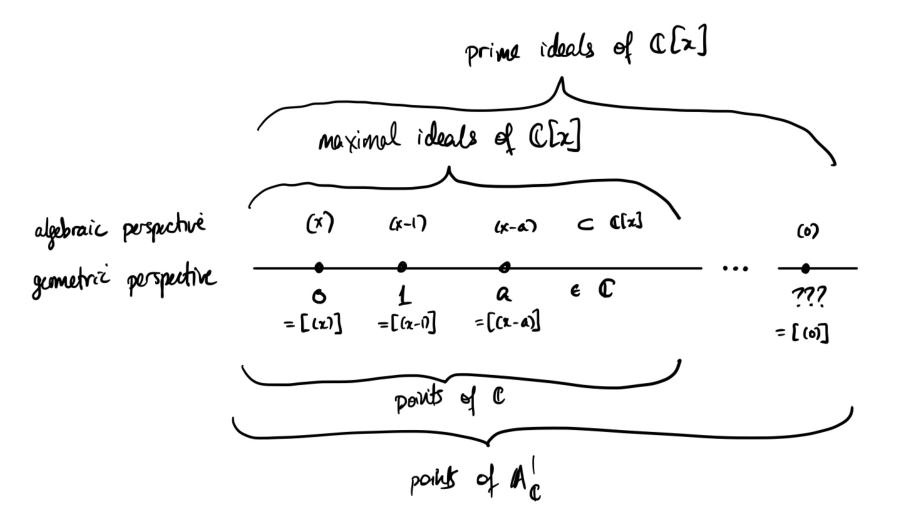
\includegraphics[width=\linewidth,height=\textheight,keepaspectratio]{Figures/complex affine line.png}
    				        \caption{The complex affine line $\A^1_{\bbC}$ (\cite{risingsea}, figure 3.1)}
    				        \label{fig: complex_affine_line}
    				    \end{figure}
    				This result generalises in an obvious manner to algebraically closed fields other than $\bbC$; so for instance, studying schemes over the field $\overline{\Q}$ of algebraic numbers might help one understand more about polynomials with rational coefficients.
    				\item \textbf{(The affine line over a separably closed but not algebraically closed field):} Let $k$ be a field that is separably closed but not algebraically closed (we can take $k = \F_p(t)^{\sep}$, for example). Then, the set of non-zero prime ideals of $\A^1_k$ need not be in bijection with $k$ itself.
    				\item \textbf{(Spectrum of the integers):} The prime ideals of $\Z$ are either generated by prime numbers themselves, or the zero ideal $(0)$. Thus, the set $\Spec \Z$ is in bijection with the \textit{union} of the set of all prime numbers and the set $\{(0)\}$. 
                \end{enumerate}
            \end{example}
        
        \subsubsection{The Zariski topology as a point-set topology} \index{Topology!Zariski}
            \begin{definition}[Zariski-closed subsets] \label{def: zariski_closed}
                Let $R$ be a commutative ring and let $\scrF$ be an arbitrary subset of $R$. Then, let us declare that sets of the following form are closed in the to-be Zariski topology:
                    $$V(\scrF) := \left\{\p \in \Spec R \mid \p \supset \scrF \right\}$$
                When it might be possible to confuse Zariski-closed subsets of different ring spectra, we will write $V_R(\scrF)$ instead of simply $V(\scrF)$.
            \end{definition}
            \begin{remark}
                Of course, sets of the form $\Spec R \setminus V(\scrF)$ are Zariski-open (that is, if we are assuming that the \href{https://ncatlab.org/nlab/show/excluded+middle}{\underline{the Law of Excluded Middle}} holds).
            \end{remark}
            
            \begin{proposition}[Well-definiteness of the Zariski topology] \label{prop: zariski_closed_well_definiteness}
                Let $R$ be an arbitrary commutative ring and assume the Law of Excluded Middle. Then, Zariski-closed subsets as defined in \ref{def: zariski_closed} actually define a topology on $\Spec R$, which of course, is called the Zariski topology.
            \end{proposition}
                \begin{proof}
                    For each subset $\scrF$ of $R$, let us write $I(\scrF)$ for the $R$-ideal generated by $\scrF$. Let us now verify the axioms defining topologies on sets one-by-one.
                        \begin{enumerate}
                            \item \textbf{(The empty set and the whole set are closed):} The empty set is just $V(R)$ and that $\Spec R$ is just $V\left((0)\right)$, which are, by definition, closed in the Zariski topology. Thus, both the empty set and the whole space are Zariski-closed.
                            \item \textbf{(Finite unions of closed sets are closed):} Let $\{V(\scrF_{\alpha})\}_{\alpha \in A}$ be a \textit{finite} set of Zariski-closed subsets of $\Spec R$ and consider the following chain of logical \textit{implications} (wherein $\p$ is a prime ideal of $R$, even though this fact can be inferred from the statements themselves):
                                $$
                                    \begin{aligned}
                                        & \p \in \bigcup_{\alpha \in A} V(\scrF_{\alpha})
                                        \\
                                        \iff & \exists \alpha \in A: \p \in V(\scrF_{\alpha})
                                        \\
                                        \iff & \exists \alpha \in A: \p \supset \scrF_{\alpha}
                                        \\
                                        \iff & \bigvee_{\alpha \in A} (\p \supset \scrF_{\alpha})
                                        \\
                                        \implies & \forall \left(f_{\alpha}\right)_{\alpha \in A} \in \prod_{\alpha \in A} \scrF_{\alpha}: \prod_{\alpha \in A} f_{\alpha} \in \p
                                        \\
                                        \iff & \bigwedge_{\left(f_{\alpha}\right)_{\alpha \in A} \in \prod_{\alpha \in A} \scrF_{\alpha}} \left(\prod_{\alpha \in A} f_{\alpha} \in \p\right)
                                        \\
                                        \iff & \p \supset \left\{\prod_{\alpha \in A} f_{\alpha} \: \bigg| \: \forall \alpha \in A: f_{\alpha} \in \scrF_{\alpha} \right\}
                                        \\
                                        \iff & \p \in V\left(\left\{\prod_{\alpha \in A} f_{\alpha} \: \bigg| \: \forall \alpha \in A: f_{\alpha} \in \scrF_{\alpha} \right\}\right)
                                    \end{aligned}
                                $$
                            wherein the fourth line, in particular, holds due to the fact that ideals, by definition, are closed under scalar multiplication by elements of their ambient rings. Now, to upgrade the fourth line to an equivalence, we can show that:
                                $$\bigwedge_{\left(f_{\alpha}\right)_{\alpha \in A} \in \prod_{\alpha \in A} \scrF_{\alpha}} \left(\prod_{\alpha \in A} f_{\alpha} \in \p\right) \implies \bigvee_{\alpha \in A} (\p \supset \scrF_{\alpha})$$
                            or, as we have assumed that the Law of Excluded Middle holds, we have the following:
                                $$
                                    \begin{aligned}
                                        & \left(\bigwedge_{\left(f_{\alpha}\right)_{\alpha \in A} \in \prod_{\alpha \in A} \scrF_{\alpha}} \left(\prod_{\alpha \in A} f_{\alpha} \in \p\right) \implies \bigvee_{\alpha \in A} (\p \supset \scrF_{\alpha})\right)
                                        \\
                                        \vdash & \left(\neg \bigwedge_{\left(f_{\alpha}\right)_{\alpha \in A} \in \prod_{\alpha \in A} \scrF_{\alpha}} \left(\prod_{\alpha \in A} f_{\alpha} \in \p\right) \implies  \neg \bigvee_{\alpha \in A} (\p \supset \scrF_{\alpha})\right)
                                    \end{aligned}
                                $$
                            meaning that we can prove the contraposition instead. To that end, consider the following:
                                $$
                                    \begin{aligned}
                                        & \neg \bigwedge_{\left(f_{\alpha}\right)_{\alpha \in A} \in \prod_{\alpha \in A} \scrF_{\alpha}} \left(\p \ni \prod_{\alpha \in A} f_{\alpha}\right)
                                        \\
                                        \implies & \bigvee_{\left(f_{\alpha}\right)_{\alpha \in A} \in \prod_{\alpha \in A} \scrF_{\alpha}} \neg \left(\p \ni \prod_{\alpha \in A} f_{\alpha}\right)
                                        \\
                                        \implies & \bigwedge_{\alpha \in A} \left(\bigvee_{f_{\alpha} \in \scrF_{\alpha}} \neg(\p \ni f_{\alpha})\right)
                                        \\
                                        \implies & \bigwedge_{\alpha \in A} \left(\neg \bigwedge_{f_{\alpha} \in \scrF_{\alpha}} (\p \ni f_{\alpha})\right)
                                        \\
                                        \implies & \bigwedge_{\alpha \in A} \neg (\p \supset \scrF_{\alpha})
                                        \\
                                        \implies & \neg \bigvee_{\alpha \in A} (\p \supset \scrF_{\alpha})
                                    \end{aligned}
                                $$
                            Thus, we have managed to show that:
                                $$\neg \bigwedge_{\left(f_{\alpha}\right)_{\alpha \in A} \in \prod_{\alpha \in A} \scrF_{\alpha}} \left(\prod_{\alpha \in A} f_{\alpha} \in \p\right) \implies  \neg \bigvee_{\alpha \in A} (\p \supset \scrF_{\alpha})$$
                            and therefore:
                                $$\p \in \bigcup_{\alpha \in A} V(\scrF_{\alpha}) \iff \p \in V\left(\left\{\prod_{\alpha \in A} f_{\alpha} \: \bigg| \: \forall \alpha \in A: f_{\alpha} \in \scrF_{\alpha} \right\}\right)$$
                            Because $\p$ was chosen arbitrarily, this implies that:
                                $$\bigcup_{\alpha \in A} V(\scrF_{\alpha}) = V\left(\left\{\prod_{\alpha \in A} f_{\alpha} \: \bigg| \: \forall \alpha \in A: f_{\alpha} \in \scrF_{\alpha} \right\}\right)$$
                            Hence, the \textit{finite} union $\bigcup_{\alpha \in A} V(\scrF_{\alpha})$ is Zariski-closed by definition, and consequently, all finite unions of Zariski-closed sets are closed in the Zariski topology themselves (since $\{\scrF_{\alpha}\}_{\alpha \in A}$ is an arbitrary fintie set of subsets of $R$). Note that the finiteness assumption on the index set $A$ is crucial, as without it, one would not be able to properly make sense of the product $\prod_{\alpha \in A} f_{\alpha}$.
                            \item \textbf{(Intersections of closed sets are closed):} Let $\{V(\scrF_{\alpha})\}_{\alpha \in A}$ be an \textit{arbitrary} set of Zariski-closed subsets of $\Spec R$ and consider the following chain of logical equivalences (wherein $\p$ is a prime ideal of $R$, and again, this fact can be deduced from the statements themselves):
                                $$
                                    \begin{aligned}
                                        & \p \in \bigcap_{\alpha \in A} V(\scrF_{\alpha})
                                        \\
                                        \iff & \forall \alpha \in A: \p \in V(\scrF_{\alpha})
                                        \\
                                        \iff & \forall \alpha \in A: \p \supset \scrF_{\alpha}
                                        \\
                                        \iff & \p \supset I\left(\bigcup_{\alpha \in A} \scrF_{\alpha}\right)
                                        \\
                                        \iff & \p \in V\left(I\left(\bigcup_{\alpha \in A} \scrF_{\alpha}\right)\right)
                                    \end{aligned}
                                $$
                            It tells us that \textit{any} prime ideal $\p$ is in an intersection of Zariski-closed subsets of $\Spec R$ defined by subsets $\scrF_{\alpha}$ of $R$ if and only if it is in the Zariski-closed subset of $\Spec R$ defined by the ideal generated by the union of the sets $\scrF_{\alpha}$, or in other words, that:
                                $$\bigcap_{\alpha \in A} V(\scrF_{\alpha}) = V\left(I\left(\bigcup_{\alpha \in A} \scrF_{\alpha}\right)\right)$$
                            In turn, this implies that the intersection of the Zariski-closed sets $V(\scrF_{\alpha})$ is itself closed in the Zariski topology, and since the index set $A$ is was chosen arbitrarily, this means that arbitrary intersections of Zariski-closed sets are themselves Zariski-closed.
                        \end{enumerate}
                    Thus, with closed sets as in definition \ref{def: zariski_closed}, the Zariski topology on prime spectra of commutative rings is well-defined.
                \end{proof}
            \begin{corollary}[Quotients are closed] \label{coro: quotients_are_closed}
                Let $R$ be a commutative ring and let $I$ be an $R$-ideal. Then, $\Spec R/I$ is homeomorphic to a Zariski-closed subset of $\Spec R$. 
            \end{corollary}
                \begin{proof}
                    This comes from a straightforward application of the third isomorphism theorem for modules.
                \end{proof}
                
            \begin{definition}[A different approach: Zariski-open sets] \label{def: zariski_open}
                Let $R$ be a commutative ring. Then, let us declare that subsets of $\Spec R$ of the following form are open in the to-be Zariski topology:
                    $$D(f) := \{\p \in \Spec R \mid \p \not \ni f\}$$
                Whenever referring to more than one ring spectra, it might be beneficial to specifically write $D_R(f)$ instead of $D(f)$.
            \end{definition}
            \begin{remark} \label{remark: basic_opens_complements}
                For any commutative ring $R$, one can show through the following logical equivalences that:
                    $$D(f) = \Spec R \setminus V\left((f)\right)$$
                wherein $\p$ is an arbitrary prime ideal of $R$:
                    $$
                        \begin{aligned}
                            & \p \in D(f)
                            \\
                            \iff & \p \in \{\q \in \Spec R \mid \q \not \ni f\}
                            \\
                            \iff & \neg(\p \ni f)
                            \\
                            \iff & \neg(\p \supset (f))
                            \\
                            \iff & \p \in \Spec R \setminus \{\q \in \Spec R \mid \q \supset (f)\}
                            \\
                            \iff & \p \in \Spec R \setminus V\left((f)\right)
                        \end{aligned}
                    $$
            \end{remark}
            
            \begin{proposition}[Well-definiteness of the Zariski topology] \label{prop: zariski_open_well_definiteness}
                Let $R$ be an arbitrary commutative ring and assume the Law of Excluded Middle. Then, Zariski-open subsets as defined in \ref{def: zariski_open} actually define a topology on $\Spec R$, which of course, is called the Zariski topology.
            \end{proposition}
                \begin{proof}
                    Let us verify the axioms defining topologies on sets one-by-one.
                        \begin{enumerate}
                            \item \textbf{(The empty set and the whole set are open):} Consider the set $D(1)$, which by definition, is given by:
                                $$D(1) := \{\p \in \Spec R \mid \p \not \ni 1\}$$
                            Because prime ideals are defined to be proper, and because proper ideals are never (multiplicatively) unital, one gets that:
                                $$D(1) = \Spec R$$
                            In other words, the whole of $\Spec R$ is open by definition. Now, consider the following:
                                $$D(0) := \{\p \in \Spec R \mid \p \not \ni 0\} = \varnothing$$
                            which holds because ideals are submodules of their ambient rings, and modules over rings must contain $0$ (as an additive identity) by definition. Thus, the empty set is also Zariski-open by definition. 
                            \item \textbf{(Unions of open sets are open):} Let $\{f_{\alpha}\}_{\alpha \in A}$ be an \textit{arbitrary} set of elements of $R$ and let us apply remark \ref{remark: basic_opens_complements} to get the following chain of logical equivalences regarding the union of the sets $D(f_{\alpha})$, wherein $\p$ is an \textit{arbitrary} prime ideal of $R$:
                                $$
                                    \begin{aligned}
                                        & \p \in \bigcup_{\alpha \in A} D(f_{\alpha})
                                        \\
                                        \iff & \bigvee_{\alpha \in A} \left(\p \in D(f_{\alpha})\right)
                                        \\
                                        \iff & \bigvee_{\alpha \in A} \neg \left(\p \in V\left((f_{\alpha})\right)\right)
                                        \\
                                        \iff & \neg \bigwedge_{\alpha \in A} \left(\p \in V\left((f_{\alpha})\right)\right)
                                        \\
                                        \iff & \p \in \Spec R \setminus \bigcap_{\alpha \in A} V\left((f_{\alpha})\right)
                                    \end{aligned}
                                $$
                            This shows that:
                                $$\bigcup_{\alpha \in A} D(f_{\alpha}) = \Spec R \setminus \bigcap_{\alpha \in A} V\left((f_{\alpha})\right)$$
                            In proposition \ref{prop: zariski_closed_well_definiteness}, we have already shown using only definition \ref{def: zariski_closed} that arbitrary intersections of Zariski-closed sets are Zariski-closed themselves; in particular, this means that $\bigcap_{\alpha \in A} V\left((f_{\alpha})\right)$ is Zariski-closed. Then, by using the Law of Excluded Middle, one can see that the complement $\Spec R \setminus \bigcap_{\alpha \in A} V\left((f_{\alpha})\right)$ is necessarily Zariski-open. Thus, arbitrary unions of Zariski-open sets are Zariski-open themselves.
                            \item \textbf{(Finite intersections of open sets are open):} Let $\{f_{\alpha}\}_{\alpha \in A}$ be an \textit{finite} set of elements of $R$ and consider the following chain of logical equivalences regarding the union of the sets $D(f_{\alpha})$, wherein $\p$ is a prime ideal of $R$:
                                $$
                                    \begin{aligned}
                                        & \neg \left(\p \in \bigcap_{\alpha \in A} D(f_{\alpha})\right)
                                        \\
                                        \iff & \neg \bigwedge_{\alpha \in A} \left(\p \in D(f_{\alpha})\right)
                                        \\
                                        \iff & \bigvee_{\alpha \in A} \neg \left(\p \in D(f_{\alpha})\right)
                                        \\
                                        \iff & \bigvee_{\alpha \in A} \left(\p \in \Spec R \setminus D(f_{\alpha})\right)
                                        \\
                                        \iff & \bigvee_{\alpha \in A} \left(\p \in V\left((f_{\alpha})\right)\right)
                                        \\
                                        \iff & \p \in \bigcup_{\alpha \in A} V\left((f_{\alpha})\right)
                                    \end{aligned}
                                $$
                            (let us note that the fifth line holds thanks to remark \ref{remark: basic_opens_complements}). Now, the contraposition of the equivalence:
                                $$\neg \left(\p \in \bigcap_{\alpha \in A} D(f_{\alpha})\right) \iff \p \in \bigcup_{\alpha \in A} V\left((f_{\alpha})\right)$$
                            is:
                                $$\neg \neg \left(\p \in \bigcap_{\alpha \in A} D(f_{\alpha})\right) \iff \neg \left(\p \in \bigcup_{\alpha \in A} V\left((f_{\alpha})\right) \right)$$
                            From this, one gets the following proof:
                                $$
                                    \begin{aligned}
                                        & \neg \neg \left(\p \in \bigcap_{\alpha \in A} D(f_{\alpha})\right) \iff \neg \left(\p \in \bigcup_{\alpha \in A} V\left((f_{\alpha})\right) \right)
                                        \\
                                        \vdash & \left(\p \in \bigcap_{\alpha \in A} D(f_{\alpha})\right) \iff \left(\p \in \Spec R \setminus \bigcup_{\alpha \in A} V\left((f_{\alpha})\right) \right) 
                                        \\
                                        \vdash & \left(\bigcap_{\alpha \in A} D(f_{\alpha}) = \Spec R \setminus \bigcup_{\alpha \in A} V\left((f_{\alpha})\right)\right)
                                    \end{aligned}
                                $$
                            Lastly, let us recall that by \ref{prop: zariski_closed_well_definiteness}, the \textit{finite} union $\bigcup_{\alpha \in A} V\left((f_{\alpha})\right)$ of Zariski-closed sets is Zariski-closed itself, meaning that by the Law of Excluded Middle, the complement $\Spec R \setminus \bigcup_{\alpha \in A} V\left((f_{\alpha})\right)$ must be Zariski-open. Thus, the union $\bigcap_{\alpha \in A} D(f_{\alpha})$ is Zariski-open. Note that the finiteness assumption on the index set $A$ is crucial, as otherwise, the union $\bigcup_{\alpha \in A} V\left((f_{\alpha})\right)$ might not be Zariski-closed.
                        \end{enumerate}
                    Thus, with open sets as in definition \ref{def: zariski_open}, the Zariski topology on prime spectra of commutative rings is well-defined.
                \end{proof}
            
            \begin{proposition}[Unifying the two definitions] \label{prop: zariski_topology_equivalence}
                By asuming the Law of Excluded Middle, one gets the same topology on spectra of commutative rings via the approaches presented in definitions \ref{def: zariski_closed} and \ref{def: zariski_open}.
            \end{proposition}
                \begin{proof}
                    Let $R$ be a commutative ring. It is sufficient to show that for each element $f \in R$, the complement $\Spec R \setminus D(f)$ is closed in the sense of definition \ref{def: zariski_closed}, or equivalently, for each subset $\scrF \subset R$, the complement $\Spec R \setminus V(\scrF)$ is open in the sense of definition \ref{def: zariski_open}. We will be attempting the second approach. To that end, let us directly the following chain of logical equivalences:
                        $$
                            \begin{aligned}
                                & \p \in \bigcup_{\alpha \in A} D(f_{\alpha})
                                \\
                                \iff & \exists \alpha \in A: \p \in D(f_{\alpha})
                                \\
                                \iff & \exists \alpha \in A: \p \in \{\q \in \Spec R \mid \q \not \ni f_{\alpha}\}
                                \\
                                \iff & \exists \alpha \in A: \p \not \ni f_{\alpha}
                                \\
                                \iff & \bigvee_{\alpha \in A} \neg\left(\p \ni f_{\alpha}\right)
                                \\
                                \iff & \neg \bigwedge_{\alpha \in A} (\p \ni f_{\alpha}) 
                                \\
                                \iff & \neg \left(\p \supset \bigcup_{\alpha \in A} \{f_{\alpha}\}\right)
                                \\
                                \iff & \neg \left(\p \supset \{f_{\alpha}\}_{\alpha \in A}\right)
                                \\
                                \iff & \p \in \Spec R \setminus \left\{\q \in \Spec R \mid \q \supset \{f_{\alpha}\}_{\alpha \in A}\right\}
                                \\
                                \iff & \p \in \Spec R \setminus V\left(\{f_{\alpha}\}_{\alpha \in A}\right)
                            \end{aligned}
                        $$
                    Thus:
                        $$\bigcup_{\alpha \in A} D(f_{\alpha}) = \Spec R \setminus V\left(\{f_{\alpha}\}_{\alpha \in A}\right)$$
                    i.e. the complement of the Zariski-closed set $V\left(\{f_{\alpha}\}_{\alpha \in A}\right)$ inside $\Spec R$ is a union of Zariski-open sets $D(f_{\alpha})$, which we know from proposition \ref{prop: zariski_open_well_definiteness} to be Zariski-open itself. As stated, this implies that definitions \ref{def: zariski_closed} and \ref{def: zariski_open} give us the same Zariski topology on prime spectra of commutative rings.
                \end{proof}
            \begin{corollary} \label{coro: zariski_basis}
                Let $R$ be a commutative ring and let $f$ denote elements of $R$. Then, the distinguished Zariski-open sets $D(f)$ form a base of the Zariski topology on $\Spec R$.
            \end{corollary}
                \begin{proof}
                    This is a direct consequence of the fact that complements of Zariski-closed sets are unions of Zariski-open sets of the form $D(f)$.
                \end{proof}
            
            We have managed to show that on each ring spectrum, there is a canonical topology, namely the Zariski topology. A naturaly follow-up question is thus: can we upgrade $\Spec$ to a functor whose domain is $\Top$ instead of $\Sets$ ? Luckily, the answer is yes, although we will need to do some work to show that this is the case. 
            \begin{proposition}[Continuous functions between spectra] \label{prop: continuous_functions_between_spectra}
                By equipping prime spectra of commutative rings with the Zariski topology (in either the sense of definition \ref{def: zariski_closed} or \ref{def: zariski_open}), one naturally gets a functor:
                    $$\Spec: \Cring^{\op} \to \Top$$
                assigning to commutative rings their respective Zariski topological spaces.
            \end{proposition}
                \begin{proof}
                    It will suffice to show that given any ring homomorphism $f: A \to B$, the induced map $\Spec f: \Spec B \to \Spec A$ is continuous, which we can do by showing that preimages of Zariski-open subsets of $\Spec A$ under $\Spec f$ are closed in $\Spec B$; in fact, we can restrict our attention to \textit{basic} open subsets of $\Spec A$ (i.e. subsets of the form $D_A(a)$, for some $a \in A$), as they form a basis for the Zariski topology on $\Spec A$. Let $D_A(a)$ be such a basic open set. It preimage under $\Spec f$ is thus the following subset of $\Spec B$:
                        $$(\Spec f)^{-1}\left(D_A(a)\right) = \{\q \in \Spec B \mid (\Spec f)(\q) \in D_A(a)\}$$
                    Writing out the definition of $D_A(a)$ (cf. definition \ref{def: zariski_open}) then gives the following chain of logical equivalences:
                        $$
                            \begin{aligned}
                                & \q \in (\Spec f)^{-1}\left(D_A(a)\right)
                                \\
                                \iff & (\Spec f)(\q) \in D_A(a)
                                \\
                                \iff & f^{-1}(\q) \in D_A(a)
                                \\
                                \iff & \neg(f^{-1}(\q) \ni a)
                                \\
                                \iff & \neg(\q \ni f(a))
                                \\
                                \iff & \q \in D_B(f(a))
                            \end{aligned}
                        $$
                    which proves that:
                        $$(\Spec f)^{-1}\left(D_A(a)\right) = D_B(f(a))$$
                    and because $D_B(f(a))$ is open by definition, so is the preimage $(\Spec f)^{-1}(D_A(a))$. As stated at the beginning, this implies that $\Spec f$ is a continuous function, and thus there exists a functor:
                        $$\Spec: \Cring^{\op} \to \Top$$
                    assigning commutative rings and homomorphisms between them to ring spectra equipped with the Zariski topology and continuous maps in between.
                \end{proof}
                
            \begin{example}[Topologically interesting ring spectra]
                \noindent
                \begin{enumerate}
                    \item \textbf{(The complex affine plane and complex affine $n$-spaces):}
                        \begin{figure}[H]
                            \centering
                            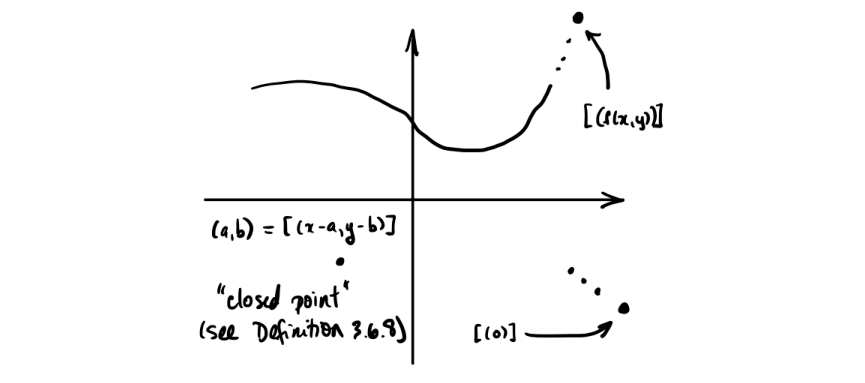
\includegraphics[width=\linewidth,height=\textheight,keepaspectratio]{Figures/complex affine plane.png}
                            \caption{The complex affine plane $\A^2_{\bbC}$ (\cite{risingsea}, figure 3.3)}
                            \label{fig: complex_affine_plane}
                        \end{figure}
                    \item \textbf{(Revisiting $\Spec \Z$):}
                        \begin{figure}[H]
                            \centering
                            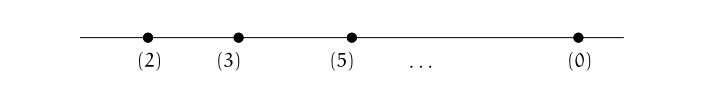
\includegraphics[width=\linewidth,height=\textheight,keepaspectratio]{Figures/Spec Z.png}
                            \caption{$\Spec \Z$ (\cite{risingsea}, figure 3.2)}
                            \label{fig: Spec_Z}
                        \end{figure}
                    \item \textbf{(A conic):}
                        \begin{figure}[H]
                            \centering
                            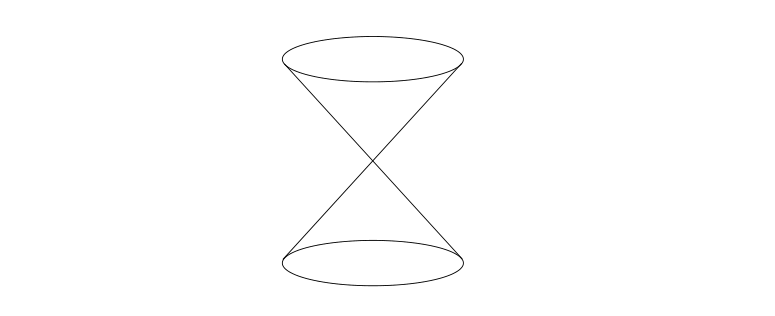
\includegraphics[width=\linewidth,height=\textheight,keepaspectratio]{Figures/conic.png}
                            \caption{A conic which is Zariski-closed inside $\A^3_{\bbC}$ (\cite{risingsea}, figure 3.4)}
                            \label{fig: conic}
                        \end{figure}
                \end{enumerate}
            \end{example}
            
            \begin{remark}[Comparing $\Spec$ and $\Spm$]
                Historically (and only because mathematicians were more interested in complex algebraic geometry back in the days), it was not the set of prime ideals of a commutative ring that was considered, but rather, the set of \textit{maximal} ideals. This was not out of \textit{na\"ivet\'e}, though. Maximal ideals enjoy being closed points in prime spectra of commutative rings (one can prove this by first looking at varieties $V(\m)$ associated to maximal ideals $\m$ of some commutative ring $R$, and then applying the definition of the (underlying set of) these varieties as spaces whose points are prime ideals containing $\m$, and then lastly, applying the usual definition of topological closures; as a corollary, one gets that prime ideals that are not maximal get sent by $\Spec$ to non-closed points in $\Spec R$), and so doing geometry with them is a lot more intuitive (albeit more restrictive as well) then doing so with all prime ideals. For instance, the underlying set of $\Spm \bbC[x]$ is precisely $\bbC$, whereas that of $\Spec \bbC[x]$ can be thought of as $\bbC \cup \{\infty\}$, i.e. as the Riemann sphere; in particular, the zero ideal $(0)$ corresponds to the point \say{at infinity}, which we denote by $\infty$. 
            \end{remark}
            
            \begin{example}[Non-isomorphic rings with homeomorphic spectra] \label{example: nonisomorphic_rings_with_the_same_spectra}
                The following examples are of non-isomorphic rings with homeomorphic prime spectra; through them, we are able to show that the functor $\Spec: \Cring^{\op} \to \Top$ is not an equivalence of categories (nor even a fully faithful inclusion). 
                \begin{enumerate}
                    \item \textbf{(Fields):} The prime spectra of any field is just the one-point space, but clearly, not all fields are isomorphic.
                    \item \textbf{(Discrete valuation rings):} The spectrum of any \href{https://en.wikipedia.org/wiki/Discrete_valuation_ring}{\underline{discrete valuation ring}} is homeomorphic to the \href{https://ncatlab.org/nlab/show/Sierpinski+space}{\underline{Sierpi\'nski space}} (to see why this is the case, firstly check that discrete valuation rings only have two prime ideals, one being the zero ideal and one being the unique maximal ideal, and that the latter is a closed point in the spectrum whereas the former is generic), but of course, not all discrete valuation rings are isomorphic to one another.
                \end{enumerate}
            \end{example}
        
        \subsubsection{Affine schemes}
            Next, we will be discussing the idea of so-call \textbf{structure sheaves}, but in order to make sense of these entities, we will need to know what $\C$-valued sheaves are for categories $\C$ more general than $\Sets$:
            \begin{definition}[$\C$-valued sheaves] \label{def: C_valued_sheaves}
                \noindent
                \begin{enumerate}
                    \item \textbf{($\C$-valued sheaves):} Let $(\S, J)$ be a site\footnote{... which is not necessarily small, as cases such as $\S \cong \Top$ and $\S \cong C^{\infty}\-\Mfd_{/\R}$ are interesting in their own rights.} and let $\C$ be a category with \textit{enough small limits} and \textit{enough filtered colimits} (the purpose of the second hypothesis is to ensure that stalks, should they exist, are well-defined); note that $\C$ need not be small. Additionally, fix an \textit{arbitrary} object $x$ of $\S$ along with a covering sieve $\calU_{/x} \in J$ thereon. Also, let $j: \S \to \Psh_{\C}(\S)$ be the Yoneda embedding. Then, a \textbf{$\C$-valued sheaf} on $(\S, J)$ is a functor $\scrF: \S^{\op} \to \C$ such that $\scrF(x) \cong \scrF\left( \underset{u \in \calU_{/x}}{\indlim} ju \right)$.
                    \item \textbf{($\C$-topoi):} $\C$-valued sheaves on a given site $(\S, J)$ form a category in the obvious manner. We shall be writing $\Sh_{\C}(\S, J)$ for this category, and such categories will be called \textbf{$\C$-topoi}, even though this is an abuse of terminology.
                \end{enumerate}
            \end{definition}
            \begin{example}[Sheaves of rings]
                The notion of sheaves of rings, which subsumes that of structure sheaves (cf. proposition \ref{prop: structure_sheaf}), follows suite from definition \ref{def: C_valued_sheaves}. Note that such constructions are well-defined, as the category of rings is both complete and cocomplete.
            \end{example}
            
            Having defined sheaves that might take values categories other than $\Sets$, let us now try to define affine schemes as locally ringed spaces whose underlying topological spaces are spectra of commutative rings, and whose structure presheaves have a certain condition imposed upon them, which happens to guarantee that:
                \begin{enumerate}
                    \item these structure presheaves are indeed sheaves (proposition \ref{prop: structure_sheaf}) with local stalks (corollary \ref{coro: structure_sheaf_properties}), and
                    \item they are unique (proposition \ref{prop: structure_sheaf_uniqueness}), which is an important feature, because ringed spaces are uniquely defined by their structure sheaves; this fact will also be used to establish the fully faithfulness of $\Spec$ as a functor from $\Cring^{\op}$ to the category $\Loc\Ringed\Spc$ of locally ringed spaces. 
                \end{enumerate}
            Our efforts will culminate in definition \ref{def: affine_schemes}.
                
            \begin{proposition}[Structure sheaves of affine schemes] \label{prop: structure_sheaf} \index{Structure sheaves}
                Let $k$ be a base commutative ring, and let $\scrO_{\Spec R}$ be \textit{a} presheaf of commutative rings on $\Ouv(\Spec R)$ determined by the following rule on objects:
                    $$\scrO_{\Spec R}(D_R(f)) \cong R_f$$
                for all element $f \in R$. Any presheaf on $\Ouv(\Spec R)$ that are defined this way is a Zariski sheaf (i.e. a sheaf on the site $\Ouv(\Spec R)$ of Zariski-open subsets of $\Spec R$), and is called \textit{a} \textbf{structure sheaf} on $\Spec R$.
            \end{proposition}
            \begin{corollary}[On the locality of stalks] \label{coro: structure_sheaf_properties}
                Let $R$ be a commutative ring and let $\p$ be an arbitrary prime ideal of $R$. Then one has the following characterisation of the stalk $\scrO_{\Spec R, \p}$ at $\p$ of the structure sheaf $\scrO_{\Spec R}$:
                    $$\scrO_{\Spec R, \p} \cong R_{\p}$$
                This shows that affine schemes are, in fact, \textit{locally} ringed spaces and not just ringed spaces. 
            \end{corollary} 
                \begin{proof}
                    Recall that the stalk $\scrF_x$ of a sheaf (of sets) $\scrF$ on a topological space $(X, \Ouv(X))$ is given by the filtered colimit indexed by the poset of open neighbourhoods of the chosen point $x \in X$:
                        $$\scrF_x \cong \underset{U \in \{V \in \Ouv(X) \mid V \ni x\}}{\indlim} \scrF(U)$$
                    By adapting this definition to the underlying Zariski-topological spaces of affine schemes, we get that:
                        $$\scrO_{\Spec R, \p} \cong \underset{U \in \{V \in \Ouv(\Spec R) \mid V \ni \p\}}{\indlim} \scrO_{\Spec R}(U)$$
                    with $\Ouv(\Spec R)$ the Zariski topology defined via open sets as in definition \ref{def: zariski_open}. In corollary \ref{coro: zariski_basis}, we have already seen how the distinguished Zariski-open sets defined in definition \ref{def: zariski_open} form a basis for the Zariski topology on commutative ring spectra, and so the above filtered colimit can be rewritten as:
                        $$\scrO_{\Spec R, \p} \cong \underset{D_R(f) \in \{V \in \Ouv(\Spec R) \mid V \ni \p\}}{\indlim} \scrO_{\Spec R}\left(D_R(f)\right)$$
                    and because $D_R(f) = \{\p \in \Spec R \mid \p \not \ni f\}$, one subsequently gets:
                        $$\scrO_{\Spec R, \p} \cong \underset{f \in \{g \in R \mid g \not \in \p\}}{\indlim} \scrO_{\Spec R}\left(D_R(f)\}\right)$$
                    Lastly we have the following isomorphism:
                        $$\scrO_{\Spec R, \p} \cong \underset{f \in \{g \in R \mid g \not \in \p\}}{\indlim} \scrO_{\Spec R}\left(D_R(f)\right) \cong \underset{f \in R \setminus \p}{\indlim} R_f \cong R_{\p}$$
                    Thus $\scrO_{\Spec R, \p} \cong R_{\p}$ as claimed.
                \end{proof}
                
            \begin{proposition}[Uniqueness of structure sheaves] \label{prop: structure_sheaf_uniqueness}
                Let $R$ be a commutative ring. Then, there is only one unique structure sheaf attached to $\Spec R$. 
            \end{proposition}
                \begin{proof}
                    Suppose to the contrary that there exist two \textit{distinct} Zariski sheaves of $R$-algebras on $R\-\Comm\Alg^{\op}$ $\scrF$ and $\scrG$ such that:
                        $$\forall f \in R: \scrF(\Spec R_f) \cong \scrG(\Spec R_f) \cong R_f$$
                    However, the localisation of any commutative at its multiplicative identity is just itself, and so:
                        $$\scrF(\Spec R) \cong \scrG(\Spec R) \cong R$$
                    for all commutative rings $R$. This means that the functors $\scrF$ and $\scrG$ are naturally isomorphic, i.e. they can not be distinct. Thus, the structure sheaf attached to a given ring spectrum is unique (up to natural isomorphisms, of course).
                \end{proof}
                
            \begin{example}[Spotting structure sheaves in the wild]
                Let $R$ be a discrete valuation ring that is a \href{https://en.wikipedia.org/wiki/Dedekind_domain}{\underline{Dedekind domain}} (so the only proper ideals of $R$ would be $(0)$ and its unique maximal ideal) with unique maximal ideal $\p$, and recall that its spectrum is (homeomorphic to) the Sierpi\'nski space (see example \ref{example: nonisomorphic_rings_with_the_same_spectra} for more details); in particular, the subset $\{(0)\}$ of $\Spec R = \{(0), \p\}$ is the only non-empty open proper subset. Now, suppose that $\scrF$ is a Zariski sheaf on $\Spec R$ given by the following formula:
                    $$
                        \scrF(U) \cong 
                        \begin{cases}
                            \text{$R$ if $U = \Spec R$}
                            \\
                            \text{$\Frac R$ if $U = \{(0)\}$}
                        \end{cases}
                    $$
                (note that discrete valuation rings are integral domains, so it makes sense to consider their fields of fractions). The point that is to be made here is that $\scrF$ qualifies as a structure sheaf on $\Spec R$. To see why this is the case, note that because $R$ has only two prime ideals, namely $(0)$ and $\p$, 
            \end{example}
            
            \begin{example}[The complex affine line]
                Recall that in example \ref{example: spectra_sets}, we have seen how a point of the complex affine line $\A^1_{\bbC}$ is either the zero ideal, or of the form $(t - a)$ for any complex number $a$; one should keep the following picture in mind:
                    \begin{figure}[H]
				        \centering
				        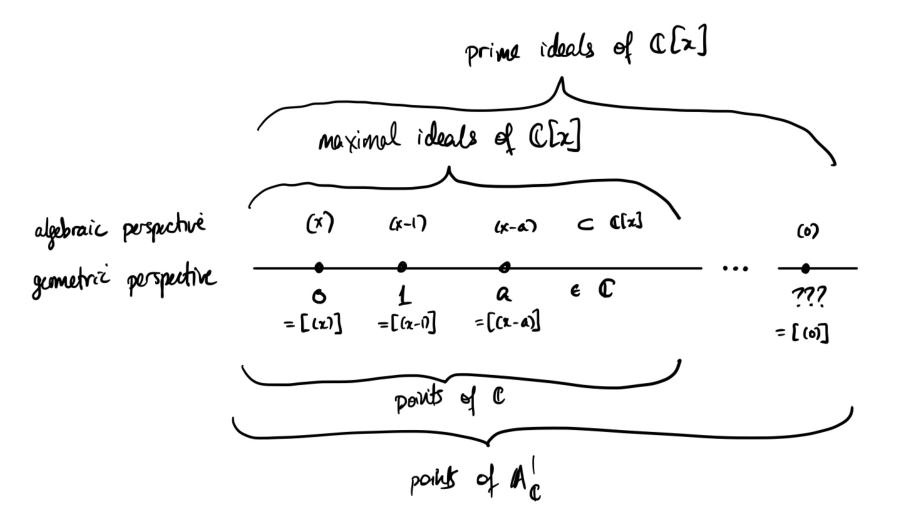
\includegraphics[width=\linewidth,height=\textheight,keepaspectratio]{Figures/complex affine line.png}
				        \caption{The complex affine line $\A^1_{\bbC}$ (\cite{risingsea}, figure 3.1)}
				        \label{fig: complex_affine_line_stalks}
				    \end{figure}
			    \noindent
			    Now, as an affine scheme, $\A^1_{\bbC}$ comes equipped with a structure sheaf $\scrO_{\A^1_{\bbC}}$, whose stalks, as shown in corollary \ref{coro: structure_sheaf_properties}, are precisely the localisations of $\bbC[t]$ at its prime ideals. There are thus two cases:
			        \begin{enumerate}
			            \item The stalk at $(0)$ is given by:
			                $$\scrO_{\A^1_{\bbC}, (0)} \cong \bbC[t]_{(0)} \cong \bbC(t)$$
		                and thus the residue field is trivially $\bbC(t)$.
			            \item At non-zero primes, the stalks of the structure sheaf $\scrO_{\A^1_{\bbC}}$ are given by the following localisations:
			                $$\scrO_{\A^1_{\bbC}, (t - a)} \cong \bbC[t]_{(t - a)}$$
		                whose elements we note to be fractions of the form $\frac{f(t)}{g(t)}$ whose denominators do not vanish at $t = a$. Now, recall that the localisation of any commutative ring at a prime ideal is a local ring, and that inside \textit{any} local commutative ring, elements in the complement of the unique maximal ideal are units; in particular, these facts imply that the elements of the complement $\bbC[t]_{(t - a)} \setminus (t - a)\bbC[t]_{(t - a)}$ are all invertible. Consequently, these elements must be fractions $\frac{f(t)}{g(t)}$ whose numerators and denominators both do not vanish at $t = a$. Thus, a reasonable description of the canonical quotient map is the evaluation map:
		                    $$\frac{f(t)}{g(t)} \mapsto \frac{f(a)}{g(a)}$$
	                    whose image is precisely $\bbC$. Therefore, the stalks of $\scrO_{\A^1_{\bbC}}$ are all isomorphic to $\bbC$.
			        \end{enumerate}
            \end{example}
        
            \begin{definition}[Affine schemes] \label{def: affine_schemes}
                An \textbf{affine scheme} is a locally ringed space that is isomorphic to one of the form $(|\Spec R|, \scrO_{\Spec R})$ for some commutative ring $R$. Morphisms of affine schemes are morphisms of locally ringed spaces, and as such, one has a full subcategory $\Sch^{\aff}$ of affine schemes within the category of locally ringed spaces. 
            \end{definition}
            
            \begin{theorem}[Isbell Duality for locally ringed spaces] \label{theorem: isbell_duality_for_locally_ringed_spaces}
                There is an adjunction as follows:
                    $$
                        \begin{tikzcd}
                        	{\Cring^{\op}} & \Loc\Ringed\Spc
                        	\arrow[""{name=0, anchor=center, inner sep=0}, "\Spec"', bend right, from=1-1, to=1-2]
                        	\arrow[""{name=1, anchor=center, inner sep=0}, "\Gamma"', bend right, from=1-2, to=1-1]
                        	\arrow["\dashv"{anchor=center, rotate=-90}, draw=none, from=1, to=0]
                        \end{tikzcd}
                    $$
            \end{theorem}
            \begin{corollary}
                The adjunction from theorem \ref{theorem: isbell_duality_for_locally_ringed_spaces} restricts down to an adjoint equivalence $\Sch^{\aff} \cong \Cring^{\op}$.
            \end{corollary}

    \subsection{The category of schemes}
        \subsubsection{Schemes}
            \begin{definition}[Schemes] \label{def: schemes}
                A \textbf{scheme} is a locally ringed space $(|X|, \scrO_X)$ such that every point $x \in |X|$ as a Zariski-open neighbourhood $U_x \ni x$ that is isomorphic to an affine scheme. Morphisms of schemes are nothing but morphisms of locally ringed spaces, meaning that schemes form a category $\Sch$ which embeds fully faithfully into the category of locally ringed spaces.
            \end{definition}
            
            \begin{proposition}[Open subschemes are open locally ringed subspaces] \label{prop: open_subschemes_are_open_locally_ringed_subspaces}
                Let $X$ be a scheme and let $U \subseteq X$ be an open locally ringed subspace. Then, $U$ will be an open subscheme of $X$. 
            \end{proposition}
                \begin{proof}
                    
                \end{proof}
            \begin{corollary}[Zariski-bases of schemes] \label{coro: zariski_bases_of_schemes}
                
            \end{corollary}
    
        \subsubsection{Properties of schemes and their morphisms}
        
        \subsubsection{Topologies on schemes; descent-theoretic results}
    
    \subsection{Varieties}

            \section{Algebraic spaces}
    \subsection{The category of algebraic spaces}
        \subsubsection{Algebraic spaces and their formal properties}
            \begin{convention}[Big sites of schemes] \label{conv: big_sites_of_schemes}
                From this point onwards, we shall be writing $(\Sch_{/S})_{\fppf}$ for the \textit{big} fppf site of a given scheme $S$. In the presence of small sites, which we denote by $(\Sch_{/S})_{\fppf}^{\petit}$, we might write $(\Sch_{/S})_{\fppf}^{\gros}$ for the sake of distinction. Likewise for the \'etale topology.
            \end{convention}
            \begin{convention}[Diagonals] \label{conv: algebraic_spaces_diagonals}
                Let $S$ be a scheme and $F$ be a presheaf of sets on $(\Sch_{/S})_{\fppf}$. We shall be denoting its \textbf{diagonal} by $\Delta_{F/S}: F \to F \x_S F$. This is the morphism of sheaves which is as follows, for all $T \in \Ob((\Sch_{/S})_{\fppf})$:
                    $$\Delta_{F/S}(T): F(T) \to F(T) \x_{S(T)} F(T)$$
                    $$t \mapsto (t, t)$$
            \end{convention}
            
            \begin{lemma}[Permanence of properties of representable morphisms] \label{lemma: permanence_of_properties_of_representable_morphisms}
                Consider sheaves on a site $(\C, J)$, which may or may not be small.
                    \begin{enumerate}
                        \item Representability of morphisms of sheaves is preserved by compositions.
                        \item Representability of morphisms of sheaves is preserved by pullbacks. Also, the diagonal of a representable morphism of sheaves is also representable.
                        \item Let $\varphi: F \to G$ be a representable morphisms of presheaves on $\C$. If $G$ satisfies $J$-descent, then so does $F$.
                    \end{enumerate}
            \end{lemma}
                \begin{proof}
                    \noindent
                    \begin{enumerate}
                        \item 
                        \item 
                        \item 
                    \end{enumerate}
                \end{proof}
            \begin{definition}[Properties of representable morphisms] \label{def: properties_of_representable_morphisms_of_fppf_sheaves}
                Denote by $\calP$ an fppf-local\footnote{Cf. \cite[\href{https://stacks.math.columbia.edu/tag/02KO}{Tag 02KO}]{stacks-project}.} property of morphisms of schemes that is stable under base-changes\footnote{See \cite[\href{https://stacks.math.columbia.edu/tag/02WE}{Tag 02WE}]{stacks-project} for a list of such properties.}. Then, one says that a representable morphism of presheaves $\varphi: F \to G$ on $(\Sch_{/S})_{\fppf}$ (for some base scheme $S$) has property $\calP$ if and only if for all schemes $U \in \Ob(\Sch_{/S})$, the canonical projection $\pr_2: F \x_G U \to U$ has property $\calP$ (note that by representability, the pullback $F \x_G U$ is an object of $\Sch_{/S}$).
            \end{definition}
            \begin{proposition}[A representability criterion for diagonals] \label{prop: representability_criterion_for_diagonals}
                Let $S$ be a scheme and let $F$ be a presheaf of sets on $(\Sch_{/S})_{\fppf}$. In addition, suppose that $U, V \in \Ob(\Sch_{/S})$ are two arbitrary $S$-schemes equipped with morphisms $u: U \to F$ and $v: V \to F$, and that the pullback $U_{u, F, v} V$ is representable by some $S$-scheme $T \in \Ob(\Sch_{/S})$. If the canonical morphism $T \to U \x_S V$ has a property $\calP$ that is fppf-local and stable under base-changes, then the diagonal $\Delta_{F/S}: F \to F \x_S F$ must be representable and have property $\calP$.
            \end{proposition}
                \begin{proof}
                    
                \end{proof}
                
            \begin{definition}[Atlases] \label{def: atlases}
                Let $S$ be a scheme and let $F$ be a presheaf of sets on $(\Sch_{/S})_{\fppf}$. An fppf (respectively, \'etale) \textbf{atlas} of $F$ is thus an \'etale surjection $U \to F$ from some scheme $U \in \Ob(\Sch_{/S})$.
            \end{definition}
            \begin{definition}[Algebraic spaces] \label{def: algebraic_spaces}
                An \textbf{algebraic space} over a scheme $S$ is a sheaf of sets on $(\Sch_{/S})_{\fppf}$ with an \'etale atlas and representable diagonal.
            \end{definition}
            \begin{remark}[Algebraic spaces are algebraic stacks]
                Later on, we shall see that algebraic spaces are the same as so-called \textbf{$0$-algebraic stacks}. More on this later, once we have discussed algebraic stacks.
            \end{remark}
            \begin{proposition}[The category of algebraic spaces] \label{prop: the_category_of_algebraic_spaces}
                For any given scheme $S$, there is a category of algebraic spaces over $S$, denoted by $\Alg\Spc_{/S}$, which is a full subcategory of $\Sh(\Sch_{S, \fppf})$. 
            \end{proposition}
                \begin{proof}
                    
                \end{proof}
                
            \begin{proposition}[(Co)limits of algebraic spaces] \label{prop: (co)limits_of_algebraic_spaces}
                For any given scheme $S$, the category $\Alg\Spc_{/S}$ of algebraic spaces over $S$ has the following (co)limits:
                    \begin{enumerate}
                        \item \textbf{(Limits):} terminal objects and finite pullbacks (and hence finite products),
                        \item \textbf{(Colimits):} arbitrary small coproducts.
                    \end{enumerate}
            \end{proposition}
                \begin{proof}
                    \noindent
                    \begin{enumerate}
                        \item \textbf{(Limits):} 
                        \item \textbf{(Colimits):} 
                    \end{enumerate}
                \end{proof}
            \begin{corollary}[Schemes are algebraic spaces] \label{coro: schemes_are_algebraic_spaces}
                For any given scheme $S$, the category $\Sch_{/S}$ of $S$-schemes is a full subcategory of $\Alg\Spc_{/S}$ which is closed under finite pullbacks.
            \end{corollary}
            \begin{remark}[A sheaf-theoretic definition of schemes] \label{remark: sheaf_theoretic_definition_of_schemes}
                In fact, it is easy to see - using the fact that the fppf topology is subcanonical - that \textit{schemes are fppf sheaves $X$ on the category of affine schemes such that their diagonals $\Delta_X$ are representable and such that they admit so-called Zariski atlases, i.e. a jointly surjective family of open immersions $U_i \hookrightarrow X$ from affine schemes $U_i$}. Note that this definition is not circular since one can define schemes either as objects of $\Cring^{\op}$ or as certain kinds of locally ringed spaces, which is a definition that makes use of only the Zariski topology on prime spectra of commutative rings and the notion of structure sheaves.
            \end{remark}
            \begin{definition}[Clopen immersions of ringed spaces] \label{def: clopen_immersions_of_ringed_spaces}
                An immersion of ringed spaces is said to be \textbf{clopen} whenever it is simultaneously closed and open.
            \end{definition}
            \begin{remark}[Clopen immersions of fppf sheaves] \label{remark: clopen_immersions_of_fppf_sheaves}
                Given definition \ref{def: clopen_immersions_of_ringed_spaces}, we can define a \textbf{clopen immersion of sheaves} on $(\Sch_{/S})_{\fppf}$ (with $S$ being some scheme) as a morphism that is representable by clopen immersions of schemes. Note that this is a well-defined notion, as open immersions and closed immersions are stable under base change (since tensor products commute with localisations and quotients) and are fppf-local (cf. \cite[\href{https://stacks.math.columbia.edu/tag/01JY}{Tag 01JY}]{stacks-project}).
            \end{remark}
            \begin{lemma}[Representability by schemes and algebraic spaces of disjoint summands] \label{lemma: representability_by_schemes_and_algebraic_spaces_of_disjoint_summands}
                Throughout, we work over a base scheme $S$.
                \begin{enumerate}
                    \item Let $F, G$ be sheaves of sets on $(\Sch_{/S})_{\fppf}$. Then, the cannical morphism of sheaves $\iota_1: F \to F \sqcup G$ (or equivalently, $\iota_2: G \to F \sqcup G$) is a clopen immersion.
                    \item Let $X$ be a $S$-scheme (respectively, an algebraic space over $S$) and suppose that there exists a disjoint set $\{F_i\}_{i \in I}$ of sheaves on $(\Sch_{/S})_{\fppf}$ such that $X \cong \coprod_{i \in I} F_i$. Then, each of the disjoint summand $F_i$ will be a clopen subscheme of $X$ (respectively, an algebraic space over $S$ such that the canonical morphism of sheaves $\iota_i: F_i \to X$ is a clopen immersion).
                    \item Let $F$ be a sheaf on $(\Sch_{/S})_{\fppf}$ such that there exists a set $\{F_i\}_{i \in I}$ of open\footnote{In the sense that the inclusions $F_i \hookrightarrow F$ are open immersions. Note that open immersions are fppf-local by virtue of being \'etale, and the reader is invited to check that indeed, open immersions are stable under base change (this is simple consequence of the fact that tensor products and localisations commute).} algebraic subspaces of $F$ such that $\coprod_{i \in I} F_i$ is an algebraic space over $S$ and that the canonically induced morphism of sheaves $\coprod_{i \in I} F_i \to F$ is surjective. In such a situation, $F$ will also be an algebraic space over $S$.
                \end{enumerate}
            \end{lemma}
                \begin{proof}
                    \noindent
                    \begin{enumerate}
                        \item 
                        \item 
                        \item 
                    \end{enumerate}
                \end{proof}
                
            \begin{definition}[\'Etale equivalence relations] \label{def: etale_equivalence_relations}
                Let $S$ be a scheme. An \textbf{\'etale equivalence relation} internal to the category $\Sch_{/S}$ of $S$-schemes (respectively, the category $\Alg\Spc_{/S}$ of algebraic spaces over $S$)\footnote{Note that both categories have all finite pullbacks.} is thus an internal equivalence relation (in the sense of definition \ref{def: equivalence_relations}) whose source and target morphisms are both \'etale.
            \end{definition}
            \begin{lemma}[Base-changing \'etale and flat equivalence relations in schemes] \label{lemma: base_changing_etale_and_flat_equivalence_relations_in_schemes}
                Let $S$ be a scheme, let $U$ be an $S$-scheme, and let $s, t: R \toto U$ be an \'etale equivalence relation on $U$ over $S$.
                    \begin{enumerate}
                        \item \textbf{(\'Etale base-changes):} Suppose that $f: U' \to U$ is an \'etale morphism of $S$-schemes and that $s', t': R' \toto U'$ is the pullback of $s, t: R \toto U$ along $f$. Then, $s', t': R' \toto U'$ will be an \'etale equivalence relation\footnote{Recall that pullbacks of internal equivalence relations are also internal equivalence relations, so $s', t': R' \toto U'$ is \textit{a priori} an equivalence relation on $U'$ over $S$ (cf. \cite[\href{https://stacks.math.columbia.edu/tag/02V8}{Tag 02V8}]{stacks-project}). Out task here is simply to establish geometric properties of the pullback $s', t': R' \toto U'$, such as whether or not it is \'etale.} on $U'$ over $S$.
                        \item \textbf{(Flat base-changes):} Suppose that the source and target morphisms $s, t: R \toto U$ are surjective, flat, and locally of finite presentation and that $f: U' \to U$ is a morphism of $S$-schemes that is flat and locally of finite presentation; in addition, denote by $s', t': R' \toto U'$ the pullback\footnote{We leave the verification of the fact that being surjective, flat, and locally of finite presentation are properties of morphisms of ($S$-)schemes which are stable under base-changes and are fppf-local up to our readers. } along $f$ of $s, t: R \toto U$. Then, the canonically induced morphism of sheaves $U'R/' \to U/R$ will be an open immersion. 
                    \end{enumerate}
            \end{lemma}
                \begin{proof}
                    \noindent
                    \begin{enumerate}
                        \item \textbf{(\'Etale base-changes):} Consider the following pullback diagrams in $\Sch_{/S}$:
                            $$
                                \begin{tikzcd}
                                	{R'} & {U'} \\
                                	R & U
                                	\arrow["{t'}"', shift right=2, from=1-1, to=1-2]
                                	\arrow["t"', shift right=2, from=2-1, to=2-2]
                                	\arrow["{f_s}"', shift right=2, from=1-1, to=2-1]
                                	\arrow["f", from=1-2, to=2-2]
                                	\arrow["\lrcorner"{anchor=center, pos=0.125}, draw=none, from=1-1, to=2-2]
                                	\arrow["s", shift left=2, from=2-1, to=2-2]
                                	\arrow["{s'}", shift left=2, from=1-1, to=1-2]
                                	\arrow["{f_t}", shift left=2, from=1-1, to=2-1]
                                \end{tikzcd}
                            $$
                        \'Etale morphisms are stable under base-changes so the canonical projections $f_s, f_t: R' \to\to R$ must be \'etale as a consequence of $f: U' \to U$ being \'etale by assumption. Compositions of \'etale morphisms are also \'etale themselves, and since $s, t: R \toto U$ are \'etale morphisms by assumption, the compositions $s \circ f_s$ and $t \circ f_t$ must also be \'etale. As such, the equivalence relation $s', t': R' \toto U'$ is \'etale. 
                        \item \textbf{(Flat base-changes):} By arguing as above and using the fact that surjectivity, flatness, and being locally of finite presentation are properties of morphisms of schemes which are stable under base-changes
                    \end{enumerate}
                \end{proof}
            \begin{proposition}[Base-chaning \'etale and flat equivalence relations in algebraic spaces] \label{prop: base_changing_etale_and_flat_equivalence_relations_in_algebraic_spaces}
                Let $S$ be a scheme, let $\calX$ be an algebraic space over $S$, and let $s, t: R \toto \calX$ be an \'etale equivalence relation on $\calX$ over $S$.
                    \begin{enumerate}
                        \item \textbf{(\'Etale base-changes):} Suppose that $f: \calX' \to \calX$ is an \'etale morphism of algebraic spaces over $\calX$ and that $s', t': R' \toto \calX'$ is the pullback of $s, t: R \toto \calX$ along $f$. Then, $s', t': R' \toto \calX'$ will be an \'etale equivalence relation on $\calX'$ over $S$.
                        \item \textbf{(Flat base-changes):} Suppose that the source and target morphisms $s, t: R \toto \calX$ are surjective, flat, and locally of finite presentation and that $f: \calX' \to \calX$ is a morphism of algebraic spaces over $S$ that is flat and locally of finite presentation; in addition, denote by $s', t': R' \toto \calX'$ the pullback along $f$ of $s, t: R \toto \calX$. Then, the canonically induced morphism of sheaves $\calX'/R' \to \calX/R$ will be an open immersion. 
                    \end{enumerate}
            \end{proposition}
            \begin{definition}[\'Etale presentations of algebraic spaces] \label{def: etale_presentations_of_algebraic_spaces}
                An \textbf{\'etale presentation} of an algebraic space $\calX$ over some scheme $S$, should it exist, is the quotient of an $S$-scheme $U$ by an \'etale equivalence relation $R$ on $U$ such that we have an isomorphism $\calX \cong U/R$ of sheaves on $(\Sch_{/S})_{\fppf}$. Phrased differently, an \'etale presentation of an algebraic space $\calX$ over some scheme $S$ is a coequaliser in $\Sh((\Sch_{/S})_{\fppf})$ of the following form, wherein $U$ and $R$ are as above:
                    $$
                        \begin{tikzcd}
                        	R & U & \calX
                        	\arrow[shift right=2, from=1-1, to=1-2]
                        	\arrow[shift left=2, from=1-1, to=1-2]
                        	\arrow["\coeq", two heads, from=1-2, to=1-3]
                        \end{tikzcd}
                    $$
            \end{definition}
            \begin{proposition}[Existence of \'etale presentation of algebraic spaces] \label{prop: existence_of_etale_presentations_of_algebraic_spaces}
                Let $S$ be a scheme, let $\calX$ be an algebraic space over $S$, and suppose that $\calX$ admits an \'etale atlas $u: U \to \calX$ by an $S$-scheme $U$ (cf. definition \ref{def: algebraic_spaces}). Then, we have the following \'etale presentation for $\calX$, wherein the two arrows $U \x_{u, \calX, u} U \toto U$ come from the canonical morphism $U \x_{u, \calX, u} U \to U \x_S U$:
                    $$
                        \begin{tikzcd}
                        	{U \x_{u, \calX, u} U} & U & \calX
                        	\arrow[shift right=2, from=1-1, to=1-2]
                        	\arrow[shift left=2, from=1-1, to=1-2]
                        	\arrow["{\coeq(u, u)}", two heads, from=1-2, to=1-3]
                        \end{tikzcd}
                    $$ 
            \end{proposition}
                \begin{proof}
                    
                \end{proof}
            \begin{proposition}[Quotients of schemes by \'etale equivalence relations are algebraic spaces] \label{prop: quotients_of_schemes_by_etale_equivalence_relations_are_algebraic_spaces}
                If $U$ is an $S$-scheme and $R$ is an \'etale equivalence relation on $U$, then not only will the sheaf $U/R$ be an algebraic space, but furthermore, the quotient morphism $U \to U/R$ will be \'etale\footnote{Because the quotient morphism $U \to U/R$ is \'etale, the \'etale presentation $R \toto U$ determines an \'etale atlas $U \to U/R$ of the algebraic space $U/R$.} surjection of sheaves on $(\Sch_{/S})_{\fppf}$. 
            \end{proposition}
                \begin{proof}
                    
                \end{proof}
                
            \begin{proposition}[Pushouts of algebraic spaces] \label{prop: puhsouts_of_algebraic_spaces}
                
            \end{proposition}
    
        \subsubsection{Properties of algebraic spaces and their morphisms}
        
        \subsubsection{Topologies on algebraic spaces; descent-theoretic results}
        
        \subsubsection{Criteria for sheaves being algebraic spaces}
    
    \subsection{Algebraic spaces over fields}

            \section{Algebraic stacks}
    \subsection{The \texorpdfstring{$2$}{}-category of algebraic stacks}
        \subsubsection{Algebraic stacks and their formal properties}
    
        \subsubsection{Properties of algebraic stacks and their morphisms}
        
        \subsubsection{Topologies on algebraic stacks; descent-theoretic results}
    
    \subsection{Moduli spaces of algebraic stacks}
        \subsubsection{Coarse moduli spaces and the Keel-Mori Theorem}
            In this subsubsection, we attempt to state and prove the Keel-Mori Theorem, which establishes a criterion for certain kinds of algebraic stacks to admit coarse moduli spaces. From there, we will discuss certain applications thereof: in particular, we will be touching on Chow's Lemma for algebraic stacks, as well as a valuative criterion for properness for algebraic stacks.
            
            Before we begin, however, we shall need to actually introduce the notion of a \say{moduli space}, which are of a certain kind of morphism from algebraic stacks to algebraic spaces. The extra conditions are imposed so that they would behave well with respect to various geometric constructions, but essentially, moduli spaces exist to exemplify the idea that algebraic stacks are geometric objects with \say{automorphisms at each point}.
            \begin{definition}[Coarse moduli spaces] \label{def: coarse_moduli_spaces}
                \cite[Section 1, pp. 1]{conrad_keel_mori_theorem_via_stacks} Let $\scrX$ be an algebraic stack over a given scheme $S$ and suppose that $\pi: \scrX \to \calX$ is a morphism to some algebraic space $\calX$ over $S$. We say that $\calX$ is a \textbf{coarse moduli space} for $\scrX$ via $\pi$ (or rather, that the morphism of algebraic stacks $\pi: \scrX \to \calX$ is a coarse moduli space for $\scrX$) if $\pi$ is initial among all morphisms from $\scrX$ to algebraic spaces over $S$ and if for all algebraically closed fields $k$ (i.e. geometric points), the canonically induced function $[\pi(k)]: [\scrX(k)] \to \calX(k)$ is a bijection.  
            \end{definition}
            \begin{remark}[On the (non)representability of coarse moduli spaces] \label{remark: (non)representability_of_coarse_moduli_spaces}
                Clearly, every algebraic space when viewed as a tautological algebraic stack is its own coarse moduli space and conversely, should a Deligne-Mumford stack admit a coarse moduli space then that modui space would be an algebraic space. The converse situation need not be true, stemming from the fact that general algebraic stacks \textit{a priori} admit only smooth atlases. 
            \end{remark}
            \begin{definition}[Fine moduli spaces] \label{def: fine_moduli_spaces}
                A \textbf{fine moduli space} over a scheme $S$ is nothing but a representable presheaf on $\Sch_{/S}$.
            \end{definition}
            \begin{remark}[On the sheafiness of moduli spaces] \label{remark: sheafiness_of_moduli_spaces}
                Many of the common Grothendieck topologies on the category of schemes (e.g. Zariski, \'etale, fppf, fpqc, etc.) are subcanonical and as such fine moduli spaces are automaticallly sheaves with respect to these topologies. 
                
                For coarse moduli spaces, the situation is a bit more subtle. By definition, algebraic spaces satisfy fppf descent and therefore, they must also satisfy \'etale and Zariski descent; a result by Gabber (cf. \cite[\href{https://stacks.math.columbia.edu/tag/0APL}{Tag 0APL}]{stacks}) tells us that algebraic spaces also satisfy fpqc descent, but this is not at all trivial. As such, coarse moduli spaces of Deligne-Mumford stacks (which are algebraic spacess) satisfy Zariski, \'etale, fppf, and fpqc descent. 
            \end{remark}
            \begin{definition}[Stability of coarse moduli spaces] \label{def: stability_of_coarse_moduli_spaces}
                \footnote{Note that this definition also makes sense for fine moduli spaces as fine moduli spaces are coarse moduli spaces by definition (as schemes are instances of algebraic spaces), but because those are nothing but schemes (which form a category with all finite pullbacks, the question of whether or not the formation of a fine moduli space is stable under base-change along representable morphisms is tautological.)}Suppose that $\pi: \scrX \to \calX$ is a coarse moduli space for some algebraic stack $\scrX$ over a given scheme $S$. We say that the formation of this coarse moduli spaces is compatible with flat (respectively, smooth, \'etale, etc.) base-changes if and only if for all flat (respectively, smooth, \'etale, etc.) morphisms $f: \calX' \to \calX$ of algebraic spaces, the canonically induced morphism $\scrX \x^2_{\pi, \calX, f} \calX' \to \calX'$ is also a coarse moduli space.   
            \end{definition}
            \begin{remark}[The importance of flat base-changes] \label{remark: flat_base_changes_of_coarse_moduli_spaces}
                Aside from encompassing the many important cases of base-change, such as smooth and \'etale base-changes, flat morphisms also arise naturally in algebraic geometry: Zariski localisations, for instance, are flat morphisms due to localisations and tensor products commuting. As such, we pay extra attention to whether or not the formation of coarse moduli spaces is preserved by flat base-changes. 
            \end{remark}
            
            \begin{definition}[Well-nigh affine algebraic stacks] \label{def: well_nigh_affine_algebraic_stacks}
                \cite[\href{https://stacks.math.columbia.edu/tag/0DUL}{Tag 0DUL}]{stacks} An algebraic stack $\scrX$ is said to be \textbf{well-nigh affine-schematic}\footnote{... or simply \textbf{well-nigh affine}.} (respecitvely, well-nigh schematic) over a given scheme $S$ if and only if there exists an affine $S$-scheme $U$ along with an atlas $U \to \scrX$ that is flat, finite (respecitvely, quasi-finite), and of finite presentation (respectively, Zariski-locally of finite-presentation) over $S$. 
            \end{definition}
            \begin{remark}
                It is clear from the definition that being well-nigh affine implies being well-nigh schematic.
            \end{remark}
            \begin{remark}[Well-nigh schematicity is fppf local] \label{remark: well_nigh_schematicity_is_fppf_local}
                Flatness, (quasi-)finiteness, and being (Zariski-locally) of finite presentation are all fppf local properties which are fppf-local and stable under base-changes along representable morphisms (cf. \cite[\href{https://stacks.math.columbia.edu/tag/02WE}{Tag 02WE}]{stacks}). Therefore, for an algebraic stack to be well-nigh affine (respectively, well-nigh schematic) is a property that is fppf-local, and hence \'etale and Zariski-local, as well as stable under base-changes along representable morphisms.
                
                Note also that because being well-nigh affine (respectively, well-nigh schematic) is Zariski-local, one can check whether or not an algebraic stack is well-nigh schematic via checking whether or not it is well-nigh affine. The notion of well-nigh schematicity is therefore redundant in practice.
            \end{remark}
            \begin{proposition}[Well-nigh affine algebraic spaces] \label{prop: well_nigh_affine_algebraic_spaces}
                A well-nigh affine algebraic space is nothing but an affine scheme. 
            \end{proposition}
                \begin{proof}
                    
                \end{proof}
            \begin{proposition}[Criteria for well-nigh affineness] \label{prop: well_nigh_affineness_criteria_for_algebraic_stacks}
                \noindent
                \begin{enumerate}
                    \item Let $f: \scrX' \to \scrX$ be an affine morphism of algebraic stacks. Then $\scrX'$ will be well-nigh affine.
                    \item Suppose that $\scrX$ is an algebraic stack over a given scheme $S$. Then, $\scrX$ is well-nigh affine over $S$ if and only if there exists a finite locally free groupoid in $S$-schemes $s, t: R \toto U$ such that $\scrX \cong [U/R]$. 
                \end{enumerate}
            \end{proposition}
                \begin{proof}
                    
                \end{proof}
            \begin{lemma}[Existence of coarse moduli spaces of well-nigh affine algebraic stacks] \label{lemma: existence_of_coarse_moduli_spaces_of_well_nigh_affine_algebraic_stacks}
                Any well-nigh affine algebraic stack $\scrX$ over a given scheme $S$ admits a coarse moduli space $\pi: \scrX \to \calX$ whose formation is stable under flat base-changes. Moreover, the morphism $\pi$ is separated, quasi-compact, and universally homeomorphic over $S$.
            \end{lemma}
                \begin{proof}
                    
                \end{proof}
            \begin{lemma}[A reduction step for the Keel-Mori Theorem] \label{lemma: keel_mori_reduction_step}
                Let $\scrX$ be an algebraic stack Zariski-locally of finite presentation, whose diagonal $\Delta_{\scrX/S}$ is quasi-compact and separated, both over some given scheme $S$. Suppose furthermore that the diagonal $\Delta_{\scrX/S}$ is quasi-finite over $S$. In such a setting, there exists a covering of $\scrX$ by a set $\{\scrX_i\}_{i \in I}$ of open algebraic substacks such that each $\scrX_i$ admits a quasi-finite, flat, and finitely presented scheme atlas $U_i \to \scrX_i$.
            \end{lemma}
                \begin{proof}
                    
                \end{proof}
                
            \begin{definition}[Inertia stacks] \label{def: inertia_stacks}
                Let $f: \scrY \to \scrX$ be a morphism of algebraic stacks over a given scheme $S$. Its associated \textbf{inertia stack} $\Inert(\scrY/\scrX)$ is given by the $2$-pullback of the diagonal $\Delta_{\scrY/\scrX}: \scrY \to \scrY \x_{\scrX} \scrY$ along itself, i.e. it fits into the following $2$-pullback square:
                    $$
                        \begin{tikzcd}
                        	{\Inert(\scrY/\scrX)} & \scrY \\
                        	\scrX & {\scrY \x_{\scrX} \scrY}
                        	\arrow["{\Delta_{\scrY/\scrX}}", from=2-1, to=2-2]
                        	\arrow["{\Delta_{\scrY/\scrX}}", from=1-2, to=2-2]
                        	\arrow[from=1-1, to=2-1]
                        	\arrow[from=1-1, to=1-2]
                        	\arrow["2"{description}, "\lrcorner"{anchor=center, pos=0.125}, draw=none, from=1-1, to=2-2]
                        \end{tikzcd}
                    $$
            \end{definition}
            \begin{proposition}[Properties of inertia stacks] \label{prop: properties_of_inertia_stacks}
                Let $f: \scrY \to \scrX$ be a morphism of algebraic stacks over a given scheme $S$. Then, not only is the inertia stack $\Inert(\scrY/\scrX)$ an algebraic stack over $S$ as well, but also, the canonical projections $\pr_1, \pr_2: \Inert(\scrY/\scrX) \toto \scrY$ are both representable by morphisms locally of finite type between algebraic space over $S$. 
            \end{proposition}
                \begin{proof}
                    
                \end{proof}
            \begin{remark}[Inertia and automorphisms] \label{remark: inertia_and_automorphisms}
                Fix an algebraic stack $\scrX$ over a given base scheme $S$ and consider the evident full $2$-category\footnote{Defined in the manner of definition \ref{def: slice_2_categories}.} $\Alg\Spc_{/\scrX} \overset{2}{\subset} \Alg\Stk_{/\scrX}$ of algebraic spaces over $\scrX$. Observe that this category is $2$-equivalent to the $2$-category 
            \end{remark}
            \begin{proposition}
                Suppose that $\scrX$ is a well-nigh affine algebraic stack and $f: \scrX' \to \scrX$ is an \'etale (respectively, \'etale and separated) morphism of between well-nigh affine algebraic stacks, both over a fixed base scheme $S$. Suppose furthermore that $f$ induces isomorphisms on automorphism groups, and recall that by virtue of being well-nigh affine, the algebraic stack $\scrX$ admit a coarse moduli space $\pi: \scrX \to \calX$ over $S$ whose formation is stable under flat base-changes and such that the morphism $\pi$ is separated, quasi-compact, and universally homeomorphic over $S$.
                
                In such a situation, there exists an \'etale (respectively, \'etale and separated) morphism $g: \calX' \to \calX$ of algebraic spaces over $S$ such that the following diagram is a $2$-pullback square of algebraic stacks over $S$:
                    $$
                        \begin{tikzcd}
                        	{\scrX'} & \scrX \\
                        	{\calX'} & \calX
                        	\arrow["\pi", from=1-2, to=2-2]
                        	\arrow["g", from=2-1, to=2-2]
                        	\arrow[from=1-1, to=2-1]
                        	\arrow["f", from=1-1, to=1-2]
                        	\arrow["\lrcorner"{anchor=center, pos=0.125}, draw=none, from=1-1, to=2-2]
                        \end{tikzcd}
                    $$
            \end{proposition}
                \begin{proof}
                    
                \end{proof}
                
            \begin{theorem}[The Keel-Mori Theorem on the existence of coarse moduli spaces] \label{theorem: keel_mori_theorem_on_the_existence_of_coarse_moduli_spaces}
                
            \end{theorem}
                \begin{proof}
                    
                \end{proof}
        
        \subsubsection{Tame algebraic stacks}
            One of the issues with the notion of (coarse) moduli spaces of algebraic stacks is that it is not very stable. For instance, it is not always the case that the formation of coarse moduli spaces - especially in positive characteristics - commutes with base-changes. As such, it is worthwhile to single out a class of algebraic stacks (so-called \say{tame algebraic stacks}) for which the formation of coarse moduli spaces is actually stable under base-changes; these algebraic stacks also behave well in other ways, but these are rather technical properties, so we thought it best to discuss them later on, once we have had all the definitions in place. 
        
        \chapter{Quasi-coherent modules}
            \begin{abstract}
                
            \end{abstract}
            
            \minitoc

            \section{A six-functor formalism for quasi-coherent modules on a scheme}
    \subsection{The category of quasi-coherent modules on a scheme; compact generation}
        Suppose that $X$ is a scheme - say, with a fixed Zariski cover:
            $$\{ f_i: \Spec A_i \to X \}_{i \in I}$$
        and that we are interested in somehow \say{patching} together the categories $A_i\mod$\footnote{... viewed as sheaves of modules on the affine schemes $\Spec A_i$ - we will explain this point of view in more details shortly.} into a global category of sheaves of modules on $X$. A \textit{na\"ive} guess might be that one should just consider the category $\scrO_X\mod$ and be done with it: after all, this is a rather good category for homological algebraic purposes, being abelian and having enough injectives.
        
        However, we can do better. Morally speaking, the category of quasi-coherent $\scrO_X$-modules - typically denoted by $\QCoh(X)$ - is obtained by taking the \say{$2$-limit} (whatever that might mean) along the pullbacks:
            $$f^*_i: \scrO_X\mod \to A_i\mod$$
        thus making it what one obtains by \say{gluing} together the module categories $A_i\mod$. As such, one of the first properties of the category $\QCoh(X)$ that more-or-less is by construction, is that locally, it has enough projectives, since each $A_i\mod$ has enough projectives; it should be noted that in general, $\QCoh(X)$ fails to have enough \say{global} projectives. Furthermore, unlike $\scrO_X\mod$, $\QCoh(X)$ is compactly generated. This is a somewhat non-trivial phenomenon, but it does mean that (co)limits of objects of $\QCoh(X)$ will be easier to handle than those of $\scrO_X\mod$. Of course, $\QCoh(X)$ retains all the nice properties of $\scrO_X\mod$, such as being abelian (in fact, $\QCoh(X)$ is AB5) and having enough injectives. We will also see that it is both complete and cocomplete, closed under extensions, and filtered colimits in $\QCoh(X)$ are exact.

        \begin{convention}
            Unless stated to be otherwise, all sites will be assumed to be small. 

            If $X$ is a scheme and $\tau$ is a topology on the category of schemes, then we will write $X_{\tau} := (\Sch_{/X})_{\tau}$ to mean the category $\Sch_{/X}$ equipped with the topology $\tau$. 
        \end{convention}

        We begin by seeing how, for any commutative ring $A$, the category $A\mod$ is the same as that of $\scrO_X$-modules for $X := \Spec A$. 
        \begin{lemma}[Sheafifying modules] \label{lemma: sheafifying_modules}
            Let $A$ be a commutative ring and set $X := \Spec A$. There is a fully faithful exact functor:
                $$A\mod \hookrightarrow \scrO_X\mod$$
            sending each $A$-module $M$ to the $\scrO_X$-module ${}^{\sh}M$ on the (small) site $X_{\Zar}$ given by:
                $${}^{\sh}M(\Spec A[f^{-1}]) := M[f^{-1}]$$
            for every $f \in A$. 
        \end{lemma}
        \begin{corollary}
            Let $A$ be a commutative, $X := \Spec A$, and consider a prime ideal $\p$ of $A$, defining a point $x \in |X|$. Then:
                $${}^{\sh}M_x \cong M_{\p}$$
        \end{corollary}
        
        Now, let us see the definition of the category of quasi-coherent modules. This can be stated more generally for any site, not simply the Zariski site of a scheme, but we will not need to work in this full generality.
        \begin{definition}[Quasi-coherent modules] \label{def: quasi_coherent_modules}
            If $A$ is a commutative ring then we define the category $\QCoh(\Spec A)$ of \textbf{quasi-coherent $\scrO_{\Spec A}$-modules} to be the essential image of the fully faithful functor $A\mod \hookrightarrow \scrO_X\mod$ from lemma \ref{lemma: sheafifying_modules}.

            If $X$ is a scheme with a Zariski cover:
                $$\{ f_i: \Spec A_i \to X \}_{i \in I}$$
            then the category $\QCoh(X)$ of quasi-coherent $\scrO_X$-modules will be the subcategory of $\scrO_X\mod$ consisting of those objects $\scrM$ such that for every $i \in I$, one has that:
                $$f_i^*\scrM \cong {}^{\sh}M_i$$
            for some $A_i$-module $M_i$.
        \end{definition}
        \begin{remark}
            $\QCoh(X)$ is a full subcategory of $\scrO_X\mod$.
        \end{remark}
        \begin{theorem}[$\QCoh$ global section functor admits right-adjoint] \label{theorem: qcoh_global_section_functor_admits_right_adjoint}
            Suppose that $X$ is a scheme with a Zariski covering:
                $$\{f_i: \Spec A_i \to X\}_{i \in I}$$
            Then, for each $i \in I$, there is an adjunction\footnote{In fact, since the functor ${}^{\sh}(-): A\mod \to \scrO_{\Spec A}\mod$ is fully faithful (cf. lemma \ref{lemma: sheafifying_modules}), this adjunction is a reflective localisation. This means that in a certain technical sense, for any scheme $X$ with a Zariski cover $\{f_i: \Spec A_i \to X\}_{i \in I}$, the process of taking local sections via the functors $\Gamma(\Spec A_i, f_i^*(-)): f_i^*\scrO_X\mod \to A_i\mod$ really is localising the category $\scrO_X\mod$ to yield $A_i\mod$.}:
                $${}^{\sh}(-): A_i\mod \leftrightarrows \scrO_X\mod: \Gamma(\Spec A_i, f_i^*(-))$$
                
            When $X := \Spec A$ is affine, these adjunctions yield us adjoint equivalences of the form:
                $${}^{\sh}(-): A\mod \leftrightarrows \QCoh(X): \Gamma(X, -)$$
        \end{theorem}
            \begin{proof}
                
            \end{proof}

        Now that we have a working definition of what a quasi-coherent module over the structure sheaf of a scheme is, let us investigate the homological properties of the category of such modules. 

        Our first agenda item is Gabber's Theorem, which tells us that for $X$ a scheme, the category $\QCoh(X)$ is a Grothendieck AB5 category - i.e. it is an abelian category that is complete and cocomplete, closed under extensions, wherein filtered colimits are exact, and it has a small generating \textit{set} - and has enough injectives. This is a non-trivial result, but very necessary as we would like to be assured that homological algebra within $\QCoh(X)$ is possible. Along the way, we will also be discussing the failure of $\QCoh(X)$ to globally possess enough projective objects; this will entail looking at locally projective modules. 
        \begin{remark}[A historical aside]
            Before complex geometry \textit{\`a la} Serre and especially before scheme theory, the kind of linear-algebraic objects that were considered over spaces were not general sheaves of modules over the structure sheaf of a space, but merely vector bundles, which we now view as finite locally free modules over the structure sheaf. 

            Let us briefly remind ourselves of some shortcomings of vector bundles. Consider a general commutative ring $A$ and the category $\Vect(A)$ of finite locally free $A$-modules., i.e. $A$-modules $\scrE$ such that for every $\p \in |\Spec A|$, the localisation $\scrE_{\p}$ is finite and free over $A_{\p}$. In general, this category fails to be abelian: e.g. \todo{Find a counter-example}
        \end{remark}

        \begin{definition}[Locally projective modules] \label{def: locally_projective_modules}
            Let $X$ be a scheme with a Zariski cover:
                $$\{f_i: \Spec A_i \to X\}_{i \in I}$$
            We say that a quasi-coherent $\scrO_X$-module $\scrM$ is \textbf{locally projective} if and only if the $A_i$-module $M_i := \Gamma(\Spec A_i, f_i^*\scrM)$ is projective for every $i \in I$. Note that this definition only makes sense for $\scrM$ being quasi-coherent, since otherwise $M_i$ might fail to be an object of $A_i\mod$.
        \end{definition}
        \begin{remark}[$\QCoh$ has enough local projectives]
            Let $X$ be a scheme with a Zariski cover:
                $$\{f_i: \Spec A_i \to X\}_{i \in I}$$
            Since each of the categories $A_i\mod$ has enough projectives, it is clear that $\QCoh(X)$ locally has enough projectives, in the sense that for every object $\scrM \in \Ob( \QCoh(X) )$, there is an epimorphism:
                $$\scrP \to \scrM$$
            from some \textit{locally} projective object $\scrP \in \Ob( \QCoh(X) )$. 
        \end{remark}
        
        \begin{definition}[Small quasi-coherent modules] \label{def: small_quasi_coherent_modules}
            Let $X$ be a scheme with a Zariski cover:
                $$\{f_i: \Spec A_i \to X\}_{i \in I}$$
            and fix some cardinal $\aleph$. Also, let $\scrM$ be a quasi-coherent $\scrO_X$-module. If each $A_i$-module $\Gamma(\Spec A_i, f_i^*\scrM)$ is generated by a set of cardinality $\leq \aleph$, then we shall say that $\scrM$ is \textbf{$\aleph$-small}. 

            Denote the full subcategory of $\QCoh(X)$ consisting of $\aleph$-small objects by $\QCoh(X)_{\leq \aleph}$.
        \end{definition}
        \begin{lemma}[Closure properties of small modules] \label{lemma: closure_properties_of_small_quasi_coherent_modules}
            Let $X$ be a scheme and fix an infinite cardinal $\aleph$. Then, $\QCoh(X)_{\leq \aleph}$ will be closed under direct sums and tensor products over $\scrO_X$.
        \end{lemma}
            \begin{proof}
                
            \end{proof}
        \begin{theorem}[Gabber's Theorem: Homological properties of $\QCoh$] \label{theorem: qcoh_homological_properties}
            Let $X$ be a scheme. Then $\QCoh(X)$ will be an AB5 category and hence will have enough injectives and all limits. 
        \end{theorem}
            \begin{proof}
                
            \end{proof}
        \begin{corollary}
            Let $X$ be a scheme. Then, the canonical fully faithful embedding:
                $$\QCoh(X) \hookrightarrow \scrO_X\mod$$
            admits a quasi-inverse right-adjoint $Q_X: \scrO_X\mod \to \QCoh(X)$, usually called the \textbf{coherator}.
        \end{corollary}
        
        Before we move on, let us consider the following meta-definition, which in itself is not quite a well-defined mathematical notion, but nevertheless is a good schematic for what a \say{good} cohomology theory should look like. Over the course of the rest of this section, we shall see how quasi-coherent modules enjoy one such cohomology theory.
        \begin{definition}[Six-functor formalisms] \label{def: six_functor_formalisms}
            A six-functor formalism is a datum satisfying the following hypotheses:
            \begin{itemize}
                \item A pair $(\C, E)$ of a finitely complete $(\infty, 1)$-category $\C$ (e.g. $\C := \Sch$) and a specified class $E \subseteq \Mor(\C)$ of morphisms which:
                \begin{itemize}
                    \item contains all isomorphisms,
                    \item is closed under pullbacks, and
                    \item is closed under compositions.
                \end{itemize}
                \item \textbf{(Functoriality):} Two $(\infty, 2)$-functors:
                    $$\Shv^*, \Shv^!: \C^{\op} \to (\infty, 1)\-\Stab\Cat_2$$
                which assign to each object $X \in \Ob(\C)$ a stable $(\infty, 1)$-category $\Shv(X)$ and to each morphism $(f: X \to Y) \in \Mor(\C)$, two respective adjunctions:
                    $$f_*: \Shv(X) \leftrightarrows \Shv(Y): f_*$$
                    $$f^!: \Shv(Y) \leftrightarrows \Shv(X): f_!$$
                At this point, we have a \textbf{four-functor formalism}; the functors $f_*$ and $f_!$ respectively, are called the \textbf{$*$- and $!$-pushforwards} respectively, whereas the functors $f^*$ and $f^!$ are the \textbf{$*$- and $!$-pullbacks}. 
                \item \textbf{(Base-change):} For each $(f: X \to Y) \in E$, the $!$-pushforward:
                    $$f_!: \Shv(X) \to \Shv(Y)$$
                is to satisfy the following property: for each $(\infty, 1)$-pullback square:
                    $$
                        \begin{tikzcd}
                        {X'} & X \\
                        {Y'} & Y
                        \arrow["{f'}"', from=1-1, to=2-1]
                        \arrow["q", from=2-1, to=2-2]
                        \arrow["p", from=1-1, to=1-2]
                        \arrow["f", from=1-2, to=2-2]
                        \arrow["\lrcorner"{anchor=center, pos=0.125}, draw=none, from=1-1, to=2-2]
                        \end{tikzcd}
                    $$
                there is a natural isomorphism of $(\infty, 1)$-functors $\Shv(X) \to \Shv(Y')$:
                    $$q^* f_! \xrightarrow[]{\cong} f'_! p^*$$
                and these natural isomorphisms should be compatible with pasting $(\infty, 1)$-pullbacks. 
                \item \textbf{(Duality):} As a stable $(\infty, 1)$-category, each $\Shv(X)$ ought to be self-dual in the sense of Lurie. Moreover, this duality ought to exchange the adjunctions $(f^* \ladjoint f_*)$ and $(f_! \ladjoint f^!)$ with one another. 
                \item \textbf{(Tensoriality):} For each $X, Y \in \Ob(\C)$, there ought to be an $(\infty, 1)$-functor:
                    $$\boxtimes_{X, Y}: \Shv(X) \tensor \Shv(Y) \to \Shv(X \x Y)$$
                (with $\Shv(X) \tensor \Shv(Y)$ being in the sense of Lurie) natural in $X, Y$, which is such that for every $X \in \Ob(\C)$ (and let us write $\Delta_X: X \to X^2$ for the diagonal thereof), the following composition defines a closed symmetric monoidal structure on $\Shv(X)$:
                    $$\Shv(X)^{\tensor 2} \xrightarrow[]{\boxtimes_{X, X}} \Shv(X^2) \xrightarrow[]{\Delta_X^*} \Shv(X)$$
                These tensor products and their corresponding internal hom-functors are the remaining two functors in the six-functor formalism. 
                    
                Furthermore, we require that the $*$-pullback:
                    $$f^*: \Shv(Y) \to \Shv(X)$$
                is $(\infty, 1)$-monoidal for each $(f: X \to Y) \in \Mor(\C)$ with respect to the aforementioned closed symmetric monoidal structures on $\Shv(Y), \Shv(X)$.

                Finally, we require that with respect to any $(f: X \to Y) \in \Mor(\C)$, $\Shv(X)$ becomes a module over the closed symmetric monoidal category $\Shv(Y)$ in the following way.  
            \end{itemize}
        \end{definition}
        \begin{example}
            Take $\C$ to be the $1$-category $\Sch_{/S}$ of schemes (viewed as a trivial $(\infty, 1)$-category) - or even the $(\infty, 1)$-category of derived schemes - over a fixed base scheme $S$. Next, consider $E$ to either be the class of open immersions or of proper morphisms; we shall write $E_{\open}$ and $E_{\proper}$ to denote these classes, respectively.

            Consider firstly:
                $$\QCoh^*: \Sch_{/S}^{\op} \to (\infty, 1)\-\Cat_2$$
            to be the $(\infty, 2)$-functor as in proposition \ref{prop: qcoh_*_pullbacks}, sending $S$-schemes $X$ to the categories of quasi-coherent $\scrO_X$-modules and sending morphisms of $S$-schemes:
                $$f: X \to Y$$
            to (t-exact) left-derived $*$-pullbacks:
                $$Lf^*: D(\QCoh(Y)) \to D(\QCoh(X))$$
            between the derived categories of $\scrO_Y, \scrO_X$-modules with quasi-coherent cohomologies, viewed as stable $(\infty, 1)$-categories; the heart of the standartd t-structures on these categories are nothing but the abelian categories $\QCoh(Y)$ and $\QCoh(X)$. 
        \end{example}

    \subsection{Functorial characterisations of properties of morphisms of schemes; the pull-push yoga for quasi-coherent modules}
        \begin{convention}
            We write $(\infty, 1)\-\Stab\Cat_r$ to mean the $(\infty, r)$-category ($r = 1, 2$) of stable $(\infty, 1)$-categories, $(\infty, 1)$-functors between them, and natural transformations between said functors when $r = 2$.
        \end{convention}
    
        As all good constructions in algebraic geometry are, the creation of quasi-coherent modules is also functorial, albeit in a slightly weak sense. 
        \begin{proposition}[$*$-pullbacks and pushforwards of quasi-coherent modules] \label{prop: qcoh_*_pullbacks}
            Fix a base scheme $S$. There is a weak $(\infty, 2)$-functor:
                $$\QCoh^*: \Sch_{/S}^{\op} \to (\infty, 1)\-\Cat_2$$
            assigning to each $X \in \Ob(\Sch_{/S})$ the category $\QCoh(X)$ as in definition \ref{def: quasi_coherent_modules} and to each $(f: X \to Y) \in \Mor(\Sch_{/S})$ the colimit-preserving pullback functor:
                $$f^*: \QCoh(Y) \to \QCoh(X)$$
            This functor admits a right-adjoint $f_*$ per the Adjoint Functor Theorem. 
        \end{proposition}

        \begin{definition}[Dual stable $(\infty, 1)$-categories] \label{def: dual_stable_(infinity, 1)_categories}
            
        \end{definition}
        
        Pushing forward along proper morphisms is rather special. For convenience, let us recall the definition of properness in the context of morphisms of schemes:
        \begin{definition}[Proper morphisms] \label{def: proper_morphisms}
            
        \end{definition}
        One should keep in mind that:
        \begin{example}
            Closed immersions are proper.
        \end{example}
        \begin{lemma}[Dualising complexes and properly supported cohomology] \label{lemma: dualising_complexes_and_properly_supported_cohomology}
            
        \end{lemma}
            \begin{proof}
                
            \end{proof}
        \begin{theorem}[Proper pushforwards] \label{theorem: proper_pushforwards}
            If $f: X \to Y$ is morphism of schemes then there shall exist a natural transformation of functors $D(\QCoh(X)) \to D(\QCoh(Y))$:
                $$Lf_! \to Rf_*$$
            which will be a natural isomorphism when $f: X \to Y$ is proper. Equivalently, there is a natural transformation:
                $$\id \to Rf^! \circ Rf_*$$
            that becomes the unit of adjunction when $f: X \to Y$ is proper. 
        \end{theorem}
            \begin{proof}
                
            \end{proof}

        The first application of functoriality is the so-called Serre's Affineness Criterion, which gives a cohomological characterisation of affine morphisms amongst all qcqs morphisms $f: X \to Y$ of schemes via a verification of whether or not the pushforward $f_*\scrO_X$ is a compact projective generator of $\QCoh(Y)$. The absolute version of this theorem - which of course does not rely on functoriality of $\QCoh$ - says that a qcqs scheme $X$ is affine if and only if $\scrO_X$ is a compact projective generator of $\QCoh(X)$.
        
        For convenience, let us firstly recall what it means for a morphism of schemes to be quasi-compact and quasi-separated.
        \begin{definition}[Quasi-compactness and quasi-separatedness] \label{def: qcqs}
            A morphism of schemes $f: X \to Y$ is \textbf{quasi-compact (qc)} if for every quasi-compact open subset $|V| \subset |Y|$, the inverse image $|f|^{-1}(|V|)$ is a quasi-compact open subset of $|X|$. Recall that a topological space $S$ is \textbf{quasi-compact} if and only if every open covering thereof is refined by a finite subcover. 

            A morphism of schemes $f: X \to Y$ is \textbf{quasi-separated (qs)} if and only if its diagonal $\Delta_{X/Y}: X \to X \x_Y X$ is qc.
        \end{definition}
        \begin{remark}
            Being qcqs for schemes is to be thought of as being analogous to being (quasi-)compact and Hausdorff in point-set topology. In particular, the notion of being qcqs is meant to mirror the fact that, only inside a Hausdorff topological space is one guaranteed that the intersection of two compact subsets is once again compact.  
        \end{remark}
        \begin{lemma} \label{lemma: affine_morphisms_are_qcqs}
            Affine morphisms of schemes are qcqs.
        \end{lemma}
        \begin{lemma}
            Let $\calA$ be a cocomplete abelian category with a compact projective generator $A$. Then $\calA$ will be equivalent to the category of left-modules over the endomorphism algebra $\calA(A, A)$:
                $$\calA \cong {}^l\calA(A, A)\mod$$
        \end{lemma}
            \begin{proof}
                
            \end{proof}
        \begin{theorem}[Compact generation of $\QCoh$ on affine schemes] \label{theorem: compact_generation_of_qcoh_on_affine_schemes}
            Let $X$ be a qcqs scheme. Then $X$ is affine if and only if $\scrO_X$ is a compact projective generator of the cocomplete abelian category $\QCoh(X)$.
        \end{theorem}
            \begin{proof}
                Clear from the fact that $\Gamma(X, \scrO_X) = \End_{\scrO_X}(\scrO_X)$ by definition.
            \end{proof}
        \begin{theorem}[Serre's Affineness Criteria] \label{theorem: serre_affineness_criteria}
            For any qcqs morphism of schemes $f: X \to Y$, the following are equivalent:
            \begin{enumerate}
                \item For any $\scrM \in \Ob(\QCoh(X))$, one has that:
                    $$i > 0 \implies R^i f_*\scrM \cong 0$$
                \item $f_*\scrO_X$ is a compact projective generator of $\QCoh(Y)$. 
                \item $f: X \to Y$ is affine\footnote{Note that $X$ is necessarily qcqs in this case (cf. lemma \ref{lemma: affine_morphisms_are_qcqs}).}.
                \item For any ideal sheaf $\scrI \subset \scrO_X$ defined by a closed subscheme $Z \subset X$, one has that:
                    $$R^1 f_*\scrI \cong 0$$
            \end{enumerate}
        \end{theorem}
            \begin{proof}
                \begin{enumerate}
                    \item Assume that 1. holds and consider $\scrM \cong \scrO_X$. By hypothesis, we have that:
                        $$i > 0 \implies R^i f_*\scrO_X \cong 0$$
                    \item 
                    \item 
                    \item 
                \end{enumerate}
            \end{proof}
        \begin{remark}
            Amongst the criteria from theorem \ref{theorem: serre_affineness_criteria}, the condition that if any ideal sheaf $\scrI \subset \scrO_X$ defined by a closed subscheme $Z \subset X$, one has that:
                $$R^1 f_*\scrI \cong 0$$
            then the morphism $f: X \to Y$ is affine deserves some attention, as it is perhaps the most closely related to how affineness is perceived in classical algebraic geometry and complex geometry. 

            A closed subscheme $Z \subset X$ consists of the vanishing loci of systems of polynomial equations generating the ideals $\Gamma(U, j^*\scrI) \subset \Gamma(U, j^*\scrO_X)$\footnote{\textit{A priori}, given a morphism of schemes $f: X \to Y$ and an ideal sheaf $\scrJ \subset \scrO_Y$, the pullback $f^*\scrJ$ is an $f^*\scrO_X$-ideal if and only if $f$ is flat, but not in general, since $f^*$ might fail to be left-exact. In this case, we are fine since open immersions are flat.}, for any open immersion $j: U \hookrightarrow X$. 
        \end{remark}

        \begin{theorem}[Extending $\QCoh$ from qc open subschemes] \label{theorem: extending_qcoh_from_qc_open_subschemes}
            Let:
                $$j: U \hookrightarrow X$$
            be a qcqs\footnote{Technically, we only need to assume quasi-compactness, since open immersions are separated and hence quasi-separated \textit{a priori}.} open immersion. Then one has a natural isomorphism of functors $D(\QCoh(X)) \to D(\QCoh(U))$:
                $$Rj^! \xrightarrow[]{\cong} Lj^*$$
            Equivalently, there is an adjunction counit:
                $$Rf^! \circ Rf_* \xrightarrow[]{\cong} \id$$
        \end{theorem}
            \begin{proof}
                
            \end{proof}

    \subsection{Cohomological base-change}

    \subsection{Duality}

    \subsection{Tensor structures}

            \section{Some applications}
    \subsection{Coherent sheaves and perfect complexes; cohomology of projective spaces}
        \begin{definition}[Coherent modules] \label{def: coherent_modules}
            Let $X$ be a scheme with a fixed Zariski covering:
                $$\{ f_i: \Spec A_i \to X \}_{i \in I}$$
            The category $\Coh(X)$ of \textbf{coherent $\scrO_X$-modules} will then be the full subcategory of $\QCoh(X)$ consisting of finite-type objects, which is to say that $\scrM \in \Ob( \QCoh(X) )$ is coherent if and only if $\Gamma(\Spec A_i, f_i^*\scrM)$ is a finite $A_i$-module for every $i \in I$.
        \end{definition}
        Even though we just gave a definition of coherent sheaves on a general scheme, we will usually be considering coherent $\scrO_X$-modules over \textit{locally Noetherian} schemes $X$, for the same reason that finitely generated modules are usually considered over Noetherian rings. 
        \begin{proposition}[Coherent modules over (locally) Noetherian schemes] \label{prop: coherent_modules_over_noetherian_schemes}
            Let $X$ be a locally Noetherian scheme. Then, an $\scrO_X$-module $\scrM$ will be coherent if and only if it is finitely presented.
        \end{proposition}
        \begin{example}
            Let $X$ be a locally Noetherian scheme. Then the structure sheaf $\scrO_X$ itself is coherent. 
        \end{example}
        \begin{example}[Incoherent rings]
            If $X$ is a scheme such that $\scrO_X$ is not coherent as a module over itself, then naturally, we shall refer to $\scrO_X$ as an \textbf{incoherent sheaf of rings}. There is the following example of such a ring, due to Brian Conrad: \href{http://math.stanford.edu/~vakil/216blog/incoherent.pdf}{http://math.stanford.edu/~vakil/216blog/incoherent.pdf}.
        \end{example}

    \subsection{Zariski's Main Theorem}
        \begin{theorem}[The Theorem of Formal Functions] \label{theorem: formal_function_theorem}

        \end{theorem}
            \begin{proof}
                
            \end{proof}

        \begin{theorem}[Zariski's Main Theorem] \label{theorem: zariski_main_theorem}
            
        \end{theorem}
            \begin{proof}
                
            \end{proof}

        \begin{theorem}[Stein's Factorisation Theorem] \label{theorem: stein_factorisation}
            
        \end{theorem}

    \subsection{The archimedean GAGA principle of Serre}
        \begin{convention}
            In this subsection, we work exclusively over $\bbC$. 
        \end{convention}

        \begin{lemma}[Complex-analytic completions of finite-type $\bbC$-algebras] \label{lemma: complex_analytic_completions_of_finite_type_C_algebras}
            There is an \textbf{analytification functor}:
                $$(-)^{\an}: \bbC\-\Comm\Alg^{\ft} \to \bbC\-\Ban\Comm\Alg^{\locconvex}$$
            from the category of finite-type $\bbC$-algebras to that of locally convex Banach $\bbC$-algebras, sending objects $A$ of the former to objects $A^{\an}$ of the former, given as the complex-analytic completion of $A$. Furthermore, this functor is compatible with base-change in the sense that, if:
                $$\phi: A \to B$$
            is a homomorphism of finite-type $\bbC$-algebras then:
                $$B^{\an} \cong (A \tensor_{A, \phi} B)^{\an} \cong A^{\an} \hattensor_{A, \phi} B$$
        \end{lemma}
            \begin{proof}
                
            \end{proof}
        \begin{remark}[Associated complex-analytic topological spaces] \label{remark: associated_complex_analytic_topological_spaces}
            Let $X$ be a finite-type $\bbC$-scheme. Since $\bbC$ is algebraically closed, closed points of $X$ are in bijection with $X(\bbC)$ by Hilbert's \textit{Nullstellensatz}. At the same time, $X(\bbC)$ - by definition - consists of all solutions to the system of polynomials in $\bbC^n$ or $\P^{n, \an}_{\bbC}$ cut out by $X$ (say, $\dim X \leq n$), so $X(\bbC)$ naturally inherits the subspace topology from the complex-analytic space $\bbC^n$ or $\P^{n, \an}_{\bbC}$. In this sense, we have that:
                $$X^{\an} := X(\bbC)$$
            is the natural complex-analytic topological space associated to the underlying topological space of $X$.

            The identification of closed points of $X$ gives rise to a natural continuous embedding:
                $$i_X: X^{\an} \to X$$
        \end{remark}
        In order to obtain complex-analytic locally ringed spaces associated to locally finite-type $\bbC$-schemes, we need also to somehow complex-analytically complete the structure sheaves of these schemes. 
        \begin{proposition}[Complex-analytic completions of locally finite-type $\bbC$-schemes] \label{prop: complex_analytic_completions_of_locally_finite_type_C_schemes}
            There is an \textbf{analytification functor}:
                $$(-)^{\an}: \Sch_{/\Spec \bbC}^{\lft} \to \An\Spc$$
                $$(X, \scrO_X) \mapsto (X^{\an}, \scrO_{X^{\an}})$$
            from the category of locally finite-type $\bbC$-schemes to that of complex-analytic spaces, determined by:
                $$\scrO_X^{\an} := (i_X^*\scrO_X)^{\an}$$
            with notations as in remark \ref{remark: associated_complex_analytic_topological_spaces}. Furthermore, if:
                $$f: X \to Y$$
            is a morphism of locally finite-type $\bbC$-schemes then we will obtain a pullback square:
                $$
                    \begin{tikzcd}
                    {X^{\an}} & {Y^{\an}} \\
                    X & Y
                    \arrow["{f^{\an}}", from=1-1, to=1-2]
                    \arrow["f", from=2-1, to=2-2]
                    \arrow["{i_X}"', from=1-1, to=2-1]
                    \arrow["{i_Y}", from=1-2, to=2-2]
                    \arrow["\lrcorner"{anchor=center, pos=0.125}, draw=none, from=1-1, to=2-2]
                    \end{tikzcd}
                $$
        \end{proposition}
            \begin{proof}
                
            \end{proof}
        \begin{lemma}[(Faithful) flatness of complex-analytifications] \label{lemma: flatness_of_complex_analytifications}
            Let $A$ be an arbitrary finite-type $\bbC$-algebra. Then $A^{\an}$ will be flat over $A$. 
        \end{lemma}
            \begin{proof}
                
            \end{proof}
        \begin{corollary} \label{coro: flatness_of_complex_analytifications}
            For any locally finite-type $\bbC$-scheme $X$, the pullback functor:
                $$i_X^*: \scrO_X\mod \to \scrO_{X^{\an}}\mod$$
            is exact. 
        \end{corollary}
        
        \begin{remark}
            Consider a morphism:
                $$f: X \to Y$$
            between schemes locally of finite type over $\Spec \bbC$. This gives rise to a pullback square of locally ringed spaces:
                $$
                    \begin{tikzcd}
                    {X^{\an}} & {Y^{\an}} \\
                    X & Y
                    \arrow["{f^{\an}}", from=1-1, to=1-2]
                    \arrow["f", from=2-1, to=2-2]
                    \arrow["{i_X}"', from=1-1, to=2-1]
                    \arrow["{i_Y}", from=1-2, to=2-2]
                    \arrow["\lrcorner"{anchor=center, pos=0.125}, draw=none, from=1-1, to=2-2]
                    \end{tikzcd}
                $$
            as stated in proposition \ref{prop: complex_analytic_completions_of_locally_finite_type_C_schemes}, which in turn gives rise to the following cohomological base-change map/spectral sequence:
                $$Li_Y^* \circ R f_* \Rightarrow R f^{\an}_* \circ Li_X^*$$
            but since the functors $i_X^*, i_Y^*$ are exact \textit{a priori} (cf. corollary \ref{coro: flatness_of_complex_analytifications}), this reduces down to a cohomological comparison map as follows:
                $$i_Y^* \circ R f_* \Rightarrow R f^{\an}_* \circ i_X^*$$
            The existence of such a natural transformation allows us to formulate a version of proper base-change in this context, which yields us cohomological comparison isomorphisms that interpolate between the Zariski and complex-analytic topologies on locally finite-type $\bbC$-schemes and their associated analytic spaces respectively (see corollary \ref{coro: GAGA_cohomological_comparison}). 
        \end{remark}
        \begin{theorem}[Relative analytification of sheaves of modules] \label{theorem: relative_analytification_of_sheaves_of_modules}
            Suppose that:
                $$f: X \to Y$$
            is a morphism between schemes locally of finite type over $\Spec \bbC$. If $f$ is proper, then the canonical natural transformation:
                $$i_Y^* \circ R f_* \Rightarrow R f^{\an}_* \circ i_X^*$$
            will be a natural isomorphism of t-exact functors $D^+(\scrO_X\mod) \to D^+(\scrO_{Y^{\an}}\mod)$.
        \end{theorem}
            \begin{proof}
                This is a result of proper base-change for general ringed spaces (see \cite[\href{https://stacks.math.columbia.edu/tag/09V4}{Tag 09V4}]{stacks-project} for now). 
            \end{proof}
        \begin{corollary}[GAGA cohomological comparison] \label{coro: GAGA_cohomological_comparison}
            When $Y \cong \Spec \bbC$ (and hence $i_Y^*$ is just the identity functor), there are isomorphisms of $\bbC$-vector spaces:
                $$H^{\bullet}(X, \scrM) \cong H^{\bullet}(X^{\an}, i_X^*\scrM)$$
            In turn, this implies that the pullback functor:
                $$i_X^*: \scrO_X\mod \to \scrO_{X^{\an}}\mod$$
            is fully faithful on top of being exact, and since both of its domain and codomain are abelian categories, this implies in particular that short exact sequences are reflected. 
        \end{corollary}

        We shall now see that when we restrict our attention to coherent modules only, the module analytification functor $i_X^*$ (for any locally finite-type $\bbC$-scheme $X$) will furthermore be essentially surjective, thus giving rise to an adjoint equivalence:
            $$i_X^*: \Coh(X) \leftrightarrows \Coh(X^{\an}): i_{X *}$$
        between the categories of coherent modules on $X$ and on $X^{\an}$, with the latter being given as the category of coherent modules on the ringed space $(X^{\an}, \scrO_{X^{\an}})$ (cf. \cite[\href{https://stacks.math.columbia.edu/tag/01BU}{Tag 01BU}]{stacks-project}). The fact that:
            $$i_X^*: \scrO_X\mod \to \scrO_{X^{\an}}\mod$$
        is fully faithful means that, should its restriction down to coherent modules:
           $$i_X^*: \Coh(X) \to \Coh(X^{\an})$$
       be well-defined (cf. lemma \ref{lemma: absolute_analytification_of_coherent_modules}) then we will be able to exploit the compact generation of $\Coh(X)$ to see that the set of (compact) generators via finite colimits of $\Coh(X^{\an})$ contains that of $\Coh(X)$ as a subset. The proof of essential surjectivity then reduces down to a proof of essential surjectivity on these generators. 
        \begin{remark}[A few reminders on coherent modules on ringed spaces]
            Again, we refer the reader to \cite[\href{https://stacks.math.columbia.edu/tag/01BU}{Tag 01BU}]{stacks-project} for a more detailed discussion, but the following list of properties is important enough for our purposes to warrant at least a mention. Suppose for a moment that $(X, \scrO_X)$ is a general ringed space and write $\Coh(X)$ to denote the category of coherent $\scrO_X$-modules.
            \begin{itemize}
                \item $\Coh(X)$ is an abelian subcategory of $\scrO_X\mod$, and this is somewhat interesting, seeing how $\QCoh(X)$ is not generally even abelian for ringed spaces, unlike for schemes where quasi-coherent modules are extremely well-behaved (cf. theorem \ref{theorem: qcoh_homological_properties})
                \item In fact, $\Coh(X)$ is closed under all extensions/short exacct sequences, and thus is a Serre subcategory of $\scrO_X\mod$ by definition.
                \item $\Coh(X)$ has enough injectives, and said injective objects are flasque. 
                \item An $\scrO_X$-module is coherent if and only if it is finitely presented.
                \item If:
                    $$f: X \to Y$$
                is a morphism between general ringed spaces and if $\scrN$ is a coherent $\scrO_Y$-module, then we will not usually be guaranteed that the pullback $f^*\scrN$ is coherent over $\scrO_X$. When $f$ is proper, though, and if $\scrM$ is some coherent $\scrO_X$-module, then the pushforward $f_*\scrM$ will in fact be coherent (cf. lemma \ref{lemma: pushforwards_of_analytic_coherent_modules}), and this is one of the reasons why having the cohomological base-change formula as in theorem \ref{theorem: relative_analytification_of_sheaves_of_modules} is important for our purposes!

                That said, there is a well-defined pullback functor:
                    $$f^*: \scrO_Y\mod^{\ft} \to \scrO_X\mod^{\ft}$$
                between the categories of finitely generated/finite-type $\scrO_Y$- and $\scrO_X$-modules. The issue mentioned above stems from the fact that the pullback of a finitely presented module is only finitely generated in general.
            \end{itemize}
            
            These properties will from now on be used without explicit mention.
        \end{remark}
        \begin{lemma}[Pushforwards of analytic coherent modules] \label{lemma: pushforwards_of_analytic_coherent_modules}
            Suppose that:
                $$f: \calX \to \calY$$
            is a morphism of complex-analytic spaces. If $f$ is proper then there will be a well-defined t-exact functor:
                $$Rf_*: D^+(\Coh(\calX)) \to D^+(\Coh(\calY))$$
        \end{lemma}
            \begin{proof}
                
            \end{proof}
        \begin{lemma}[Absolute analytification of coherent modules] \label{lemma: absolute_analytification_of_coherent_modules}
            Let $X$ be a locally finite-type $\bbC$-scheme. Then, there is a well-defined functor:
                $$i_X^*: \Coh(X) \to \Coh(X^{\an})$$
            (i.e. the pullback functor $i_X^*: \scrO_X\mod \to \scrO_{X^{\an}}\mod$ in particular does send coherent $\scrO_X$-modules to coherent $\scrO_{X^{\an}}$-modules).
        \end{lemma}
            \begin{proof}[Sketch]
                $i_X^*$ is exact (cf. corollary \ref{coro: GAGA_cohomological_comparison}), so it preserves compactness of objects. 
            \end{proof}
        \begin{theorem}[Relative analytification of coherent modules] \label{theorem: relative_analytification_of_coherent_modules}
            Suppose that:
                $$f: X \to Y$$
            is a morphism between schemes locally of finite type over $\Spec \bbC$. If $f$ is proper, then the canonical natural transformation:
                $$i_Y^* \circ R f_* \Rightarrow R f^{\an}_* \circ i_X^*$$
            will be a natural isomorphism of t-exact functors $D^+(\Coh(X)) \to D^+(\Coh(Y^{\an}))$.

            When $Y \cong \Spec \bbC$, the above implies that:
                $$H^{\bullet}(X, \scrM) \cong H^{\bullet}(X^{\an}, i_X^*\scrM)$$
            are finite-dimensional $\bbC$-vector spaces for any coherent $\scrO_X$-module $\scrM$.
        \end{theorem}
        \begin{remark}[\textit{D\'evissage}]
            Let us recall Chow's Lemma, which says that should $S$ be a Noetherian base scheme and $\pi: X \to S$ be a proper $S$-scheme, then there will exist a projective $S$-scheme $\pi': X' \to S$ along with a morphism of $S$-schemes:
                $$f: X' \to X$$
            for which there is a \textit{dense} open subscheme $U \subset X$ such that:
                $$X' \x_{f, X} U \cong U$$
            If, in addition, both $X$ and $X'$ are irreducible then $f$ will be birational. Furthermore, if $X$ is reduced, irreducible, or integral, then the same can be assumed for $X'$; in particular, this means that if $X$ is a variety (i.e. when all those adjectives are satisfied and $S$ is the spectrum of a field) then we can assume without loss of generality that $X'$ too is a variety over the same field.

            Using Chow's Lemma, and letting $S := \Spec \bbC$, we see that any proper algebraic $\bbC$-variety $Y$ is birationally equivalent to a projective $\bbC$-variety $X$, for which there is some closed immersion:
                $$j_X: X \hookrightarrow \P^n_{\bbC}$$
            We know that the abelian category:
                $$\Coh(\P^n_{\bbC})$$
            is generated via finite colimits by finitely many (compact) objects (namely Serre's twisting line bundles)\footnote{This statement remains true when we replace $\bbC$ with an arbitrary commutative ring.}, 
        \end{remark}

        \begin{theorem}[Compact generation of coherent modules over analytifications] \label{theorem: compact_generation_of_coherent_modules_over_analytifications}
            For any locally finite-type proper $\bbC$-scheme $X$, any coherent $\scrO_{X^{\an}}$-module $\scrM$ admits a 
        \end{theorem}
            \begin{proof}
                
            \end{proof}
        The following is a corollary to a combination of corollary \ref{coro: GAGA_cohomological_comparison} and theorem \ref{theorem: compact_generation_of_coherent_modules_over_analytifications}.
        \begin{corollary}[Serre's GAGA]
            For any locally finite-type proper $\bbC$-scheme $X$, there is an adjoint equivalence of categories:
                $$i_X^*: \Coh(X) \leftrightarrows \Coh(X^{\an}): i_{X *}$$
        \end{corollary}
            
        \begin{appendices}
            \chapter{Fibred categories, descent, and stacks}
                \begin{abstract}
            
                \end{abstract}
                
                \minitoc
                
                \section{Fibred categories}
    \subsection{Generalities on \texorpdfstring{$2$}{}-categories}
        \subsubsection{\textit{Pr\'elude}: Internal categories}
            \begin{definition}[Spans] \label{def: spans} \index{Spans}
                \noindent
                \begin{enumerate}
                    \item \textbf{(Spans):} A \textbf{span} (also known as a \textbf{correspondence}) from an object $x$ to another object $y$ via an object $s$ inside a given category $\C$ is a diagram therein that is of the following form:
                        $$
                            \begin{tikzcd}
                            	s & y \\
                            	x
                            	\arrow["f"', from=1-1, to=2-1]
                            	\arrow["g", from=1-1, to=1-2]
                            \end{tikzcd}
                        $$
                    wherein the tip $s$ is some \textit{choice} of object of $\C$. As any span with either or both arrow therein being an identity is just a normal morphism, the notion of spans can be thought of as a generalisation of morphisms.  
                    \item \textbf{(Categories of spans):} Within a category $\C$ with pullbacks, one can compose, say, a span from $x$ to $y$ via $s$ with another from $y$ to $z$ via $s'$ via taking the pullback of the \say{inner} arrows in the manner depicted by the following diagram:
                        $$
                            \begin{tikzcd}
                            	{s \x_{g, y, f'} s'} & {s'} & z \\
                            	s & y \\
                            	x
                            	\arrow["f"', from=2-1, to=3-1]
                            	\arrow["g"', from=2-1, to=2-2]
                            	\arrow["{f'}", from=1-2, to=2-2]
                            	\arrow["{g'}", from=1-2, to=1-3]
                            	\arrow[from=1-1, to=2-1]
                            	\arrow[from=1-1, to=1-2]
                            	\arrow["\lrcorner"{anchor=center, pos=0.125}, draw=none, from=1-1, to=2-2]
                            \end{tikzcd}
                        $$
                    to obtain a so-called \say{composite} span from $x$ to $z$ via $s \x_{g, y, f'} s'$ (which visually, can be thought of either as the upper \say{roof} or the big \say{roof} covering the two smaller ones - that being the previously specified spans from $x$ to $y$ via $s$ and the span from $y$ to $z$ via $s'$ - in the above diagram); alternatively, one might visualise this composition via the following commutative diagram of spans:
                        $$
                            \begin{tikzcd}
                            	x & y & z
                            	\arrow["{(f,g)}", "\shortmid"{marking}, from=1-1, to=1-2]
                            	\arrow["{(f' g')}", "\shortmid"{marking}, from=1-2, to=1-3]
                            \end{tikzcd}
                        $$
                    With the use of this style of composition, one obtains, for every category $\C$ with pullbacks in tandem with a choice of natural number $n \geq 1$, a (lax) \textbf{$n$-category of spans} $\Span^{\leq n}(\C)$ that is defined via:
                        \begin{enumerate}
                            \item objects being those of $\C$ itself,
                            \item $1$-morphisms being spans between objects, which shall henceforth be known as $1$-spans,
                            \item and for all $2 \leq k \leq n$, $k$-morphisms, which shall henceforth be called $k$-spans, being $k$-cells between $(k-1)$-morphisms; for instance, a $2$-span between two $1$-spans is a commutative diagram of the following form:
                                $$
                                    \begin{tikzcd}
                                        \bullet \arrow[rd] \arrow[rdd, bend right] \arrow[rrd, bend left] &                             &         \\
                                                                                                          & \bullet \arrow[d] \arrow[r] & \bullet \\
                                                                                                          & \bullet                     &        
                                    \end{tikzcd}
                                $$
                        \end{enumerate}
                \end{enumerate}
            \end{definition}
            \begin{convention}[Regarding notations] \label{conv: span_notations}
                Obviously, writing out spans explicitly takes up a lot of effort and frankly, these diagrams can get confusing rather quickly. However, a quick observation tells us that because composites of spans are given by pullbacks, they actually satisfy the universal property of products taken in the arrow category of some given span category. That is to say, given an ambient category $\C$ with all pullbacks and two composable spans:
                    $$
                        \begin{tikzcd}
                        	& \bullet & \bullet \\
                        	\bullet & \bullet \\
                        	\bullet
                        	\arrow["f"', from=2-1, to=3-1]
                        	\arrow["g", from=2-1, to=2-2]
                        	\arrow["{f'}", from=1-2, to=2-2]
                        	\arrow["{g'}", from=1-2, to=1-3]
                        \end{tikzcd}
                    $$
                therein, their composite:
                    $$
                        \begin{tikzcd}
                        	\bullet & \bullet & \bullet \\
                        	\bullet & \bullet \\
                        	\bullet
                        	\arrow["f"', from=2-1, to=3-1]
                        	\arrow["g"', from=2-1, to=2-2]
                        	\arrow["{f'}", from=1-2, to=2-2]
                        	\arrow["{g'}", from=1-2, to=1-3]
                        	\arrow[from=1-1, to=2-1]
                        	\arrow[from=1-1, to=1-2]
                        	\arrow["\lrcorner"{anchor=center, pos=0.125}, draw=none, from=1-1, to=2-2]
                        \end{tikzcd}
                    $$
                is nothing but the product:
                    $$
                        \begin{tikzcd}
                        	{(f, g) \x (f', g')} & {(f', g')} \\
                        	{(f, g)}
                        	\arrow[dashed, from=1-1, to=2-1]
                        	\arrow[dashed, from=1-1, to=1-2]
                        \end{tikzcd}
                    $$
                in $\Mor\left(\Span^{\leq 1}(\C)\right)$ (which will probably be commonly written as $\Span^{\leq 1}(\C)_1$ from now on, so as to make the notion of spans fit snuggly into the language of internal categories, and also to cut back on parentheses) Therefore, our proposition of an alternative notation is as follows: the composition of two spans $(f, g)$ and $(f', g')$ shall instead be denoted by $(f, g) \x (f', g')$.
            \end{convention}
            \begin{convention}[Associators]
                Fix a \textit{weak} $n$-category $\C$, with $n \geq 1$. Now, for all $1 \leq k \leq n$ and all triples of \textit{composable} $(k - 1)$-morphisms $f, g, h$ of $\C$, let us call the $k$-cell:
                    $$(fg)h \to f(gh)$$
                (which we note to be invertible thanks to the weakness assumption on $\C$) a \textbf{$k$-associator}. An associator is called \textbf{trivial} if and only if it is an identity. See \href{https://ncatlab.org/nlab/show/associator}{\underline{here}} for more details. 
            \end{convention}
            \begin{remark}[Associators in span categories]
                Since pullbacks are merely unique up to unique isomorphisms, $k$-associators in the $n$-category $\Span^{\leq n}(\C)$ of spans of a given category $\C$ with pullbacks are generally non-trivial, but they are invertible. This implies that $n$-categories of spans are \textit{weak} $n$-categories, as opposed to simply being lax $n$-categories, but generally they are not strict $n$-categories. 
            \end{remark}
            
            \begin{proposition}[Limits and colimits of spans]
                
            \end{proposition}
        
            \begin{definition}[Internal categories] \label{def: internal_categories}
                Let $\E$ be a category with \textit{enough pullbacks}. A category \textbf{internal} to $\E$ is then a pair $(C_0, C_1)$ of objects of $\E$ defined via the following data:
                    \begin{enumerate}
                        \item \textbf{(Objects and morphisms):} An object of \textbf{objects} $C_0 \in \E$ and an object of \textbf{arrows} $C_1 \in \E$, both are to be viewed as internal analogues of the collections of objects and arrows in the definition of categories.
                        \item \textbf{(Composition):} 
                            \begin{enumerate}
                                \item \textbf{(Sources and targets):} From the object of arrows $C_1$ to the object of objects $C_0$, there are two morphisms $s, t$ as follows, known as the \textbf{source} and \textbf{target} maps:
                                    $$
                                        \begin{tikzcd}
                                        	{C_1} & {C_0}
                                        	\arrow["s", shift left=2, from=1-1, to=1-2]
                                        	\arrow["t"', shift right=2, from=1-1, to=1-2]
                                        \end{tikzcd}
                                    $$
                                which, respectively, assign to each arrow $f \in C_1$ (which, along with similar instances, shall be viewed as a \href{https://ncatlab.org/nlab/show/generalized+element}{\underline{generalised elements}} for the sake of linguistic convenience) its domain and codomain objects in $C_0$.
                                \item \textbf{(Units):} From the object of objects $C_0$ to the object of arrows $C_1$, there is a distinguished morphism:
                                    $$e: C_0 \to C_1$$
                                called the \textbf{unit map} which assigns to each object $x \in C_0$ (again, viewed as a generalised element) the identity $\id_x: x \to x$ thereon, which we note to be an a generalised element of the object of arrows $C_1$ (hence the codomain of $e$ is $C_1$).
                                \item \textbf{(Composition of arrows):} There is a monoidal composition operation (in the sense of monoidal categories):
                                    $$\mu: C_1 \x_{s, C_0, t} C_1 \to C_1$$
                                satisfying the following conditions specified by commutative diagrams in $\E$:
                                    \begin{enumerate}
                                        \item \textbf{(Identities do not alter domains and codomains):}
                                            $$
                                                \begin{tikzcd}
                                                	{C_0} & {C_1} && {C_0} & {C_1} \\
                                                	& {C_0} &&& {C_0}
                                                	\arrow["e", from=1-1, to=1-2]
                                                	\arrow["{\id_{C_0}}"', from=1-1, to=2-2]
                                                	\arrow["s", from=1-2, to=2-2]
                                                	\arrow["{\id_{C_0}}"', from=1-4, to=2-5]
                                                	\arrow["t", from=1-5, to=2-5]
                                                	\arrow["e", from=1-4, to=1-5]
                                                \end{tikzcd}
                                            $$
                                        \item \textbf{(Sources and targets of compositions):} The source of a composition $g \mu f \in C_1$ should be that of $f$ (the former), wheareas its target should be that of $g$ (the latter): 
                                            $$
                                                \begin{tikzcd}
                                                	& {C_1 \x_{s, C_0, t} C_1} & {C_1} && {C_1 \x_{s, C_0, t} C_1} & {C_1} \\
                                                	{} & {C_1} & {C_0} && {C_1} & {C_0}
                                                	\arrow["s", from=1-3, to=2-3]
                                                	\arrow["s", from=2-2, to=2-3]
                                                	\arrow["{\pr_2}"', from=1-2, to=2-2]
                                                	\arrow["{\pr_1}", from=1-2, to=1-3]
                                                	\arrow["t", from=1-6, to=2-6]
                                                	\arrow["t", from=2-5, to=2-6]
                                                	\arrow["{\pr_1}"', from=1-5, to=2-5]
                                                	\arrow["{\pr_1}", from=1-5, to=1-6]
                                                \end{tikzcd}
                                            $$
                                        \item \textbf{(Associativity):} 
                                            $$
                                                \begin{tikzcd}
                                                	& {C_1 \x_{s, C_0, t} C_1 \x_{s, C_0, t} C_1} & {C_1 \x_{s, C_0, t} C_1} \\
                                                	{} & {C_1 \x_{s, C_0, t} C_1} & {C_1}
                                                	\arrow["\mu", from=1-3, to=2-3]
                                                	\arrow["\mu", from=2-2, to=2-3]
                                                	\arrow["{\id_{C_1} \x_{s, C_0, t} \mu}"', from=1-2, to=2-2]
                                                	\arrow["{\mu \x_{s, C_0, t} \id_{C_1}}", from=1-2, to=1-3]
                                                \end{tikzcd}
                                            $$
                                        \item \textbf{(Left and right-unitarity):} 
                                    \end{enumerate}
                                        $$
                                            \begin{tikzcd}
                                            	{C_0 \x_{C_0} C_1} & {C_1 \x_{s, C_0, t} C_1} & {C_1 \x_{C_0} C_0} \\
                                            	& {C_1}
                                            	\arrow["\mu", from=1-2, to=2-2]
                                            	\arrow["{\pr_2}"', from=1-1, to=2-2]
                                            	\arrow["{\pr_1}", from=1-3, to=2-2]
                                            	\arrow["{\e \x_{C_0} \id_{C_1}}", from=1-1, to=1-2]
                                            	\arrow["{\id_{C_1} \x_{C_0} e}"', from=1-3, to=1-2]
                                            \end{tikzcd}
                                        $$
                                with the latter three specifying the monoidality of the composition operation $\mu$.
                            \end{enumerate}
                    \end{enumerate}
            \end{definition}
            
            \begin{remark}[Internal categories vs. subcategories]
                    
            \end{remark}
            
            \begin{remark}[Another formulation: Internal categories as monads on spans] \label{remark: internal_categories_alt_def}
                Definition \ref{def: internal_categories} gives us a perfectly fine idea of what one might mean by \say{internal categories}. However, it is manifestly rather clunky. Therefore, the author has taken the liberty to provide one alternative formulation of the notion of internal categories.
                
                We refer the reader to definition \ref{def: spans} and the discussion that follows for necessary information on the paradigm of spans; in particular, let us recall that spans are only well-defined inside categories with pullbacks (which is a slightly stronger condition than the assumption in definition \ref{def: internal_categories} that the ambient category as merely \textit{enough} pullbacks). 
                    
                Now, let $\E$ be an ambient category with all pullbacks, and subsequently, let us define a category $C$ internal to $\E$ as being the same as a monad in the weak $2$-category $\Span^{\leq 2}(\E)$ of spans on $\E$. Why would this even resemble a reasonable definition of categories internal to a given category $\E$ ? For starters, recall that a monad is an endomorphism satisfying so-called \say{monoidal multiplication}. Therefore, an internal category $C$ inside a given ambient category $\E$ is first and foremost an endomorphism on a choice of object, and because the weak $2$-category in which we are trying to build monads is one of spans, our endomorphism should be a \say{roof} diagram whose two \say{lower} vertices are the same. By consulting definition \ref{def: internal_categories}, one sees that an obvious choice is the source-target span:
                    $$
                        \begin{tikzcd}
                        	{C_1} & {C_0} \\
                        	{C_0}
                        	\arrow["s"', from=1-1, to=2-1]
                        	\arrow["t", from=1-1, to=1-2]
                        \end{tikzcd}
                    $$
                (recall that objects in span categories are those of the underlying category and morphisms are span themselves; cf. definition \ref{def: spans}); let us denote this span by the \textit{unordered} pair $(s, t)$. Now, is this endomorphism indeed a monad in $\Span^{\leq 2}(\E)$ ? First of all, one can certainly compose $(s, t)$ with itself thanks to the assumption that $\E$ has all pullbacks: said composition is nothing but the composite span $(s, t) \x (s, t)$ (see remark \ref{conv: span_notations} for an explanation of this notation); let us denote this composition by $\mu$, and note that it is precisely a $2$-cell from $(s, t) \x (s, t)$ to $(s, t)$, a fact that can be proven via consideration of the following universal diagram:
                    $$
                        \begin{tikzcd}
                        	{(s, t) \x (s, t)} & {(s, t)} \\
                        	{(s, t)} & {(s, t)}
                        	\arrow[dashed, from=1-1, to=2-1]
                        	\arrow[dashed, from=1-1, to=1-2]
                        	\arrow[Rightarrow, no head, from=1-2, to=2-2]
                        	\arrow[Rightarrow, no head, from=2-1, to=2-2]
                        	\arrow["\mu", from=1-1, to=2-2]
                        \end{tikzcd}
                    $$
                and thanks to the universal property of products, this composition is trivially asociative. There is also a unit $e := (\id_{C_0}, \id_{C_0}) \x (s, t)$ which satisfies the following commutative diagram:
                    $$
                        \begin{tikzcd}
                        	{(\id_{C_0}, \id_{C_0}) \x (s, t)} & {(s, t) \x (s, t)} & {(s, t) \x (\id_{C_0}, \id_{C_0})} \\
                        	& {(s, t)}
                        	\arrow["\mu", from=1-2, to=2-2]
                        	\arrow["{\pr_2}"', from=1-1, to=2-2]
                        	\arrow["{\pr_1}", from=1-3, to=2-2]
                        	\arrow["{e \x \id_{(s, t)}}", from=1-1, to=1-2]
                        	\arrow["{\id_{(s, t)} \x e}"', from=1-3, to=1-2]
                        \end{tikzcd}
                    $$
                This proves that the composition $\mu$ is also unital, and hence all the monad axioms have been shown to hold. Incidentally, we have also managed to show via this discussion, that monads in the category of spans in a category with pullbacks are nothing but internal categories.
            \end{remark}
            
            \begin{definition}[Internal functors] \label{def: internal_functors}
                Let $\E$ be an ambient category with \textit{enough pullbacks} and let $C, D$ be two categories that are internal to $\E$.
                    \begin{enumerate}
                        \item \textbf{(Internal functors):} Internal functors between categories that are internal to a given ambient category (with enough pullbacks) are defined in the exact same way as the internal definition of functors between ordinary categories. See \href{https://ncatlab.org/nlab/show/functor#InternalDefinition}{\underline{here}} for a reminder.
                        \item \textbf{(Anafunctors):} (Ah yes, the Axiom of Choice. Making lives miserable as always) While the general definition of internal functors might not have lit any bulbs in the deparment of choice, one should definitely keep in mind that the notion of essential surjectivity definitely does depend on choice: if:
                            $$F: C \to D$$
                        is an essentially surjective internal functor, then one will be able to \textit{choose} objects $x \in C_0$ such that:
                            $$Fx \cong y$$
                        for every object $y \in D_0$. As the ramifications of the Axiom of Choice tend to be unfamiliar to those not actively involved in the logic community (including the author, who had to consult a few nLab articles too), let us quickly explain why anafunctors are needed in place of the above \textit{na\"ive} notion of internal functors; particularly, we would like to know what mappings between internal categories might look like when our ambient category does not host the Axiom of Choice, such as when its size is an inaccessible cardinal ($\Top$ is one particular case). To that end, \todo[inline]{Write about why the Axiom of Choice breaks essentially surjective internal functors}
                        
                        Now, let us define an \textbf{anafunctor} $F$ between two internal categories $C$ and $D$ of a given category $\E$ - should such a mapping exist - to be a span (i.e. a $1$-morphism in $\Span^{\leq 2}(\E)$; cf. definition \ref{def: spans}) of internal categories:
                            $$
                                \begin{tikzcd}
                                	{F} & {D} \\
                                	{C}
                                	\arrow[from=1-1, to=2-1]
                                	\arrow[from=1-1, to=1-2]
                                \end{tikzcd}
                            $$
                        which shall be interpreted as the following composition of spans in $\E$:
                            $$
                                \begin{tikzcd}
                                	\bullet & \bullet & {D_1} & {D_0} \\
                                	\bullet & {F_0} & {D_0} \\
                                	{C_1} & {C_0} \\
                                	{C_0}
                                	\arrow[from=3-1, to=4-1]
                                	\arrow[from=3-1, to=3-2]
                                	\arrow[from=2-2, to=3-2]
                                	\arrow[from=2-2, to=2-3]
                                	\arrow[from=1-3, to=2-3]
                                	\arrow[from=1-3, to=1-4]
                                	\arrow[from=2-1, to=3-1]
                                	\arrow[from=2-1, to=2-2]
                                	\arrow[from=1-1, to=2-1]
                                	\arrow[from=1-1, to=1-2]
                                	\arrow[from=1-2, to=2-2]
                                	\arrow[from=1-2, to=1-3]
                                	\arrow["\lrcorner"{anchor=center, pos=0.125}, draw=none, from=1-2, to=2-3]
                                	\arrow["\lrcorner"{anchor=center, pos=0.125}, draw=none, from=1-1, to=2-2]
                                	\arrow["\lrcorner"{anchor=center, pos=0.125}, draw=none, from=2-1, to=3-2]
                                \end{tikzcd}
                            $$
                        (see remark \ref{remark: internal_categories_alt_def} for a description of internal categories as spans - or to be more precise, monads in span categories). Note that in the event that $\E$ also has products (or equivalently, terminal objects), anafunctors between any given pair of internal categories $C$ and $D$ always exist: one can simply take $F_0$ to be $C_0 \x D_0$. Also, let us draw attention to the fact that this definition is logically independent of the notion of internal functors, and therefore we have not committed circular reasoning.
                    \end{enumerate}
            \end{definition}
            \begin{remark}[Categories of internal categories] \label{remark: categories_of_internal_categories}
                Via the above notion of anafunctors and the idea presented in remark \ref{remark: internal_categories_alt_def} that internal categories and monads in span categories are the same thing, one can rather easily show that categories internal to a given ambient category $\E$ (with pullbacks) form a weak $2$-category, which is precisely equivalent to the category of monads in $\Span^{\leq 2}(\E)$. In notations, one writes:
                    $$1\-\Cat(\E) \cong \Monad\left(\Span^{\leq 2}(\E)\right)$$
            \end{remark}
            \begin{remark}[Categories as monoids] \label{remark: categories_as_monoids}
                Remark \ref{remark: internal_categories_alt_def}, definition \ref{def: internal_functors}, remark \ref{remark: categories_of_internal_categories}, and remark \ref{conv: span_notations} in tandem tell us that internal to every ambient category $\E$ with pullbacks, there is a symmetric monoidal category $1\-\Cat(\E)$ of categories internal to $\E$ whose monoidal multiplication is given by $2$-spans from squares:
                    $$
                        \begin{tikzcd}
                        	{C_1 \x_{s, C_0, t} C_1} \\
                        	& {C_1} & {C_0} \\
                        	& {C_0}
                        	\arrow["s", from=2-2, to=3-2]
                        	\arrow["t"', from=2-2, to=2-3]
                        	\arrow[from=1-1, to=3-2]
                        	\arrow[from=1-1, to=2-3]
                        	\arrow["\mu"{description}, from=1-1, to=2-2]
                        \end{tikzcd}
                    $$
                and whose monoidal unit is given pointwise on each internal category:
                    $$
                        \begin{tikzcd}
                        	{C_1} & {C_0} \\
                        	{C_0}
                        	\arrow["s"', from=1-1, to=2-1]
                        	\arrow["t", from=1-1, to=1-2]
                        \end{tikzcd}
                    $$
                by a $2$-span from $(\id_{C_0}, \id_{C_0}) \to (s,t)$:
                    $$
                        \begin{tikzcd}
                        	{C_0} \\
                        	& {C_1} & {C_0} \\
                        	& {C_0}
                        	\arrow["s", from=2-2, to=3-2]
                        	\arrow["t"', from=2-2, to=2-3]
                        	\arrow["e"{description}, from=1-1, to=2-2]
                        	\arrow["{\id_{C_0}}"', from=1-1, to=3-2]
                        	\arrow["{\id_{C_0}}", from=1-1, to=2-3]
                        \end{tikzcd}
                    $$
                Both of which (together) are subjected to the usual monoidal axioms (cf. definition \ref{def: internal_categories}). In other words, internal categories inside a given ambient category $\E$ are nothing but monoids in $1\-\Cat(\E)$. This is a rather neat observation, as it allows us to view morphisms between internal categories not too differently from monoid homomorphism. 
            \end{remark}
            
            \begin{definition}[Internal groupoids] \label{def: internal_groupoids}
                Let $\E$ be a category with pullbacks and let:
                    $$
                        \begin{tikzcd}
                        	{\scrG_1} & {\scrG_0} \\
                        	{\scrG_0}
                        	\arrow["s"', from=1-1, to=2-1]
                        	\arrow["t", from=1-1, to=1-2]
                        \end{tikzcd}
                    $$
                be the data of a category internal to $\E$. Such an internal category is an \textbf{internal groupoid} if in addition, there exists an arrow:
                    $$i: \scrG_1 \to \scrG_1$$
                called the \textbf{inverse map}, that renders the following diagram in $\E$ commutative:
                    $$
                        \begin{tikzcd}
                        	{\scrG_1} \\
                        	& {\scrG_1} & {\scrG_0} \\
                        	& {\scrG_0}
                        	\arrow["i"{description}, from=1-1, to=2-2]
                        	\arrow["t"', from=1-1, to=3-2]
                        	\arrow["s", from=2-2, to=3-2]
                        	\arrow["t"', from=2-2, to=2-3]
                        	\arrow["s", from=1-1, to=2-3]
                        \end{tikzcd}
                    $$
                (i.e. the inverse map switches the source and target of a given internal morphism), and such that the following diagrams of spans - telling us that multiplication with inverses returns the identity regardless of whether the process is carried out from the left and from the right - commute:
                    $$
                        \begin{tikzcd}
                        	{\scrG_1} & {\scrG_1 \x_{s, \scrG_0, t} \scrG_1} & {\scrG_1 \x_{s, \scrG_0, t} \scrG_1} \\
                        	{\scrG_0} && {\scrG_1}
                        	\arrow["{\mu_{\scrG}}", from=1-3, to=2-3]
                        	\arrow["{i \x_{s, \scrG_0, t} \id_{\scrG_1}}", from=1-2, to=1-3]
                        	\arrow["{\Delta_{\scrG_1/\scrG_0}}", from=1-1, to=1-2]
                        	\arrow["t"', from=1-1, to=2-1]
                        	\arrow["e", from=2-1, to=2-3]
                        \end{tikzcd}
                    $$
                    $$
                        \begin{tikzcd}
                        	{\scrG_1} & {\scrG_1 \x_{s, \scrG_0, t} \scrG_1} & {\scrG_1 \x_{s, \scrG_0, t} \scrG_1} \\
                        	{\scrG_0} && {\scrG_1}
                        	\arrow["{\mu_{\scrG}}", from=1-3, to=2-3]
                        	\arrow["{\id_{\scrG_1} \x_{s, \scrG_0, t} i}", from=1-2, to=1-3]
                        	\arrow["{\Delta_{\scrG_1/\scrG_0}}", from=1-1, to=1-2]
                        	\arrow["s"', from=1-1, to=2-1]
                        	\arrow["e", from=2-1, to=2-3]
                        \end{tikzcd}
                    $$
                In other words, groupoids internal to a category with pullbacks $\E$ are group objects in the category $1\-\Cat(\E)$ of categories internal to $\E$ (which we note to have all finite products; cf. remark \ref{conv: span_notations}).
            \end{definition}
            \begin{remark}[On the inverse maps of internal groupoids]
                Definition \ref{def: internal_groupoids}, while standard, suffers from a few issues. For one, it is not very clear how internal groupoids should be thought of as groups in categories of internal categories. Also, the inverse map defining the structure of each internal groupoid, at least according to definition \ref{def: internal_groupoids}, is rather non-functorial. Luckily, these two problems can be easily resolved. 
                
                Firstly, let us note that the inverse map $i_{\scrG}: \scrG_1 \to \scrG_1$ associated to an internal groupoid:
                    $$
                        \begin{tikzcd}
                        	{\scrG_1} & {\scrG_0} \\
                        	{\scrG_0}
                        	\arrow["s"', from=1-1, to=2-1]
                        	\arrow["t", from=1-1, to=1-2]
                        \end{tikzcd}
                    $$
                is not just a morphism in the ambient category satisfying certain conditions, but actually a $2$-span: it is a $2$-span from the $1$-span $(s,t): \scrG_1 \toto \scrG_0$ to the $1$-span $(t,s): \scrG_1 \toto \scrG_0$. Thus, one can meaningfully think of the inverse map on $\scrG$ as an anafunctor from $\scrG$ to itself. Second of all, recall that in remark \ref{remark: categories_as_monoids}, we have seen how internal categories are actually monoid objects, which in particular, means that composition of arrows therein behaves in a manner similar to multiplication. So actually, all that we need to do is to somehow configure inverse maps so that they would act like multiplicative inverses, which would in turn help us formally recognise internal groupoids as group objects; we shall leave the drawing of the relevant commutative diagrams to the reader, as they can be rather easily inferred from the ones in definition \ref{def: internal_groupoids}. 
            \end{remark}
        
            \begin{definition}[Equivalence relations] \label{def: equivalence_relations}
                Let $\E$ be a \textit{finitely complete} category ($\Sets$ or general topoi, or $1\-\Cat$, for instance)
                    \begin{enumerate}
                        \item \textbf{(Binary relations):} A \textbf{binary relation} $R$ from an object $X$ to another object $Y$ of $\E$ is a $1$-span:
                            $$
                                \begin{tikzcd}
                                	R & Y \\
                                	X
                                	\arrow[from=1-1, to=2-1]
                                	\arrow[from=1-1, to=1-2]
                                \end{tikzcd}
                            $$
                        such that $R$ is a subobject of $X \x Y$. 
                        \item \textbf{(Equivalence relations):} An \textbf{equivalence relation} (also known as a congruence) $R$ on an object $X$ of $\E$ is a binary relation from $X$ to itself which also happens to be an internal groupoid. 
                        \item \textbf{(Quotients):} The coequaliser of an (internal) equivalence relation is known as a \textbf{quotient object}. That is, the quotient $Q$ of an object $X$ by an equivalence relation $R$ is the following coequaliser in $\E$:
                            $$
                                \begin{tikzcd}
                                	R & X & Q
                                	\arrow["s", shift left=2, from=1-1, to=1-2]
                                	\arrow["t"', shift right=2, from=1-1, to=1-2]
                                	\arrow[dashed, from=1-2, to=1-3]
                                \end{tikzcd}
                            $$
                        Of course, quotients are only guaranteed to exist if and only if $\E$ has enough coequalisers. 
                    \end{enumerate}
            \end{definition}
        
        \subsubsection{\texorpdfstring{$2$}{}-categorical constructions}
            \begin{definition}[$2$-categories and $2$-functors] \label{def: 2_categories_and_2_functors}
                
            \end{definition}
            \begin{definition}[$(2, k)$-categories] \label{def: (2, k)_categories} 
                A $(2, k)$-category (for $0 \leq k \leq 2$) is a $2$-category wherein all $(k + 1)$-morphisms are invertible.
            \end{definition}
            \begin{definition}[$2$-natural transformations] \label{def: 2_natural_transformations}
                
            \end{definition}
            \begin{definition}[Natural modifications] \label{def: natural_modifications}
                
            \end{definition}
            \begin{remark}[$2$-categories of $2$-functors] \label{remark: 2_categories_of_2_functors}
                
            \end{remark}
            
            \begin{definition}[$2$-commutative diagrams] \label{def: 2_commutative_diagrams}
                Let $\scrK$ be a $2$-category. A $2$-commutative diagram therein is thus a square as follows, wherein there exists a $2$-isomorphism $\eta: p'f \Rightarrow pg$:
                    $$
                        \begin{tikzcd}
                        	{y'} & y \\
                        	{x'} & x
                        	\arrow["{p'}"', from=1-1, to=2-1]
                        	\arrow["f", from=2-1, to=2-2]
                        	\arrow["g", from=1-1, to=1-2]
                        	\arrow["p", from=1-2, to=2-2]
                        	\arrow["\exists \eta", shorten <=8pt, shorten >=8pt, Rightarrow, from=2-1, to=1-2]
                        \end{tikzcd}
                    $$
            \end{definition}
            
            \begin{definition}[Strict and weak $2$-categories and $2$-functors] \label{def: strict_and_weak_2_categoriesand_2_functors}
                \noindent
                \begin{enumerate}
                    \item \textbf{(Strict and weak $2$-categories):} Let $\scrK$ be a $2$-category. One says that it is \textbf{strict} if compositions of (pairs of) $1$-morphisms are unique up to (necessarily unique) $2$-equalities, and \textbf{weak} if compositions of (pairs of) $1$-morphisms are unique only up to $2$-isomorphisms.
                    \item \textbf{(Strict and weak $2$-functors):}
                \end{enumerate}
            \end{definition}
            \begin{example}
                
            \end{example}
            
            Strictly speaking, the following notion ought to be known as that of $(2, 1)$-pullbacks, but since we shall not be encountering so-called \say{\textit{lax} $2$-pullbacks} (or any lax $2$-(co)limits for that matter), we shall be lazy and simply write \say{$2$-pullbacks} to mean \say{$(2, 1)$-pullbacks}.
            \begin{definition}[$2$-pullbacks] \label{def: 2_pullbacks}
                
            \end{definition}
            \begin{example}[$2$-pullbacks in $1\-\Cat_2$] \label{example: 2_pullbacks_in_the_2_category_of_categories}
                The $2$-category $1\-\Cat_2$ whose objects are $1$-categories, whose $1$-morphisms are functors, and whose $2$-morphisms are natural transformations, has all $2$-pullbacks.
            \end{example}
    
    \subsection{(Co)fibred categories}
        \subsubsection{Slice \texorpdfstring{$2$}{}-categories and prefibrations}
            \begin{definition}[Slice $2$-categories] \label{def: slice_2_categories}
                Let $\scrK$ be a $2$-category and let $x \in \Ob(\scrK)$ be an object therein. Then, we define the \textbf{slice} $2$-category $\scrK_{/x}$ to be the $2$-category wherein:
                    \begin{itemize}
                        \item the objects are $1$-morphisms $(f: y \to x) \in 1\-\Mor(\scrK)$,
                        \item the $1$-morphisms $\varphi: (y', f') \to (y, f)$ are $1$-commutative triangles of $1$-morphisms $(f': y' \to x), (f: y \to x) \in 1\-\Mor(\scrK)$ in $\scrK$ of the following form:
                            $$
                                \begin{tikzcd}
                                	{y'} && y \\
                                	& x
                                	\arrow["\varphi", from=1-1, to=1-3]
                                	\arrow["{f'}"', from=1-1, to=2-2]
                                	\arrow["f", from=1-3, to=2-2]
                                \end{tikzcd}
                            $$
                        \item and the $2$-morphisms between $1$-morphisms $\varphi, \psi: (y', f') \to (y, f)$ are $2$-morphisms $(\eta: \psi \Rightarrow \varphi) \in 2\-\Mor(\scrK)$ such that the following diagram is $2$-commutative:
                            $$
                                \begin{tikzcd}
                                	{y'} && y \\
                                	& x
                                	\arrow["{f'}"', from=1-1, to=2-2]
                                	\arrow["f", from=1-3, to=2-2]
                                	\arrow[""{name=0, anchor=center, inner sep=0}, "\varphi"', bend right, from=1-1, to=1-3]
                                	\arrow[""{name=1, anchor=center, inner sep=0}, "\psi", bend left, from=1-1, to=1-3]
                                	\arrow["\eta"', shorten <=3pt, shorten >=3pt, Rightarrow, from=1, to=0]
                                \end{tikzcd}
                            $$
                    \end{itemize}
            \end{definition}
            \begin{example}[Over-categories] \label{example: over_categories}
                Let $\C$ be a category and let $1\-\Cat_2$ be the $2$-category with $1$-categories, functors, and natural transformations as objects, $1$-morphisms, and $2$-morphisms respectively. Then, there is a natural slice $2$-category $(1\-\Cat_2)_{/\C}$ wherein the objects are functors $p: \scrS \to \C$, $1$-morphisms are the evident $1$-commutative triangles of functors, and $2$-morphisms between $1$-morphisms $F, G: (\scrS', p') \to (\scrS, p)$ are natural transformations $\eta \in \Nat(F, G)$ such that $p(\eta_y) \cong \id_{p'(y)}$ for all $y \in \Ob(\scrS')$, i.e. such that the following square is $2$-commutative:
                    $$
                        \begin{tikzcd}
                        	{p'(y)} & {p(F(y))} \\
                        	{p'(y)} & {p(G(y))}
                        	\arrow["{p(\eta_y)}", from=1-2, to=2-2]
                        	\arrow[from=1-1, to=1-2]
                        	\arrow["{\id_{p'(y)}}"', from=1-1, to=2-1]
                        	\arrow[from=2-1, to=2-2]
                        	\arrow[shorten <=8pt, shorten >=8pt, Rightarrow, from=2-1, to=1-2]
                        \end{tikzcd}
                    $$
            \end{example}
            \begin{proposition}[$2$-pullbacks in slice $2$-categories] \label{prop: 2_pullbacks_in_slice_2_categories}
                Let $\scrK$ be a $2$-category with $2$-pullbacks. Then for any $x \in \Ob(\scrK)$, the slice $2$-category $\scrK_{/x}$ shall also possess all $2$-pullbacks.
            \end{proposition}
                \begin{proof}
                            
                \end{proof}
            \begin{corollary}[$2$-pullbacks of over-categories] \label{coro: 2_pullbacks_of_over_categories}
                If $\C$ is any $1$-category then the $2$-category $(1\-\Cat_2)_{/\C}$ will have all $2$-pullbacks.
            \end{corollary}
            
            \begin{definition}[Prefibrations] \label{def: prefibrations}
                Consider a $1$-functor $p: \scrS \to \C$ between $1$-categories $\scrS$ and $\C$ is a \textbf{prefibration} if and only if it is surjective on the level of both objects and ($1$-)morphisms. 
            \end{definition}
            \begin{remark}[Op-prefibrations] \label{remark: op_prefibrations}
                It is easy to see that every prefibration $p: \scrS \to \C$ defines a so-called \textbf{op-prefibration} $p^{\op}: \scrS^{\op} \to \C^{\op}$, which is nothing but the functor $p^{\op}$ viewed as a prefibration of $\scrS^{\op}$ over $\C^{\op}$.
            \end{remark}
            \begin{remark}[Fibres of prefibrations] \label{remark: fibres_of_prefibrations}
                Consider a prefibration $p: \scrS \to \C$, viewed as a $1$-morphism of $1\-\Cat_2$, and recall that $1\-\Cat_2$ admits $1$-terminal objects, namely categories that are equivalent to the singleton category $\pt$, as well as $2$-pullbacks. By viewing objects $U \in \Ob(\C)$ as functors $U: \pt \to \C$, one can define \textbf{fibres} of the prefibration $p: \scrS \to \C$ as $2$-pullbacks of the following kind:
                    $$
                        \begin{tikzcd}
                        	{\scrS_U} & \scrS \\
                        	\pt & \C
                        	\arrow["U", from=2-1, to=2-2]
                        	\arrow["p", from=1-2, to=2-2]
                        	\arrow["{p_U}"', from=1-1, to=2-1]
                        	\arrow[from=1-1, to=1-2]
                        	\arrow["2"{description}, "\lrcorner"{anchor=center, pos=0.125}, draw=none, from=1-1, to=2-2]
                        \end{tikzcd}
                    $$
                It is then easy to see that $\scrS_U$ is the category wherein the objects are objects $x \in \scrS$ such that $p(x) = U$ and the morphisms are morphisms $(\varphi: y \to x) \in \Mor(\scrS)$ such that $p(\varphi) = \id_U$, and as such one ought to view $p_U: \scrS_U \to \pt$ as the unique functor from $\scrS_U$ to the singleton category whose only object is $U$ and whose only morphism is $\id_U$. Therefore, one can instead define prefibrations as functors $p: \scrS \to \C$ with non-empty fibres in the sense above and identify them by the families of $2$-pullbacks $\{\scrS \x^2_{p, \C, U} \pt\}_{U \in \Ob(\C)}$.
            \end{remark}
            \begin{remark}[The $2$-category of prefibrations]
                By definition, prefibrations $p: \scrS \to \C$ are objects of the $2$-category $(1\-\Cat_2)_{/\C}$, and so we might be tempted to declare that there is a $2$-full subcategory $\Pre\Fib(\C) \overset{2}{\subset} (1\-\Cat_2)_{/\C}$ spanned by prefibrations over $\C$, and indeed there is. To check that this is the case, one can verify that given any $1$-morphism $(F: (\scrS', p') \to (\scrS, p)) \in 1\-\Mor((1\-\Cat_2)_{/\C})$ and any object $U \in \C$, there exists a functor $F_U: \scrS'_U \to \scrS_U$ making the following diagram $2$-commutative in $1\-\Cat_2$:
                    $$
                        \begin{tikzcd}
                        	{\scrS'_U} &&&& {\scrS_U} \\
                        	{\scrS'} &&&& \scrS \\
                        	&& \pt \\
                        	&& \C
                        	\arrow["{p'}"', from=2-1, to=4-3]
                        	\arrow["U", from=3-3, to=4-3]
                        	\arrow["{p'_U}"', from=1-1, to=3-3]
                        	\arrow["\lrcorner"{anchor=center, pos=0.125}, draw=none, from=1-1, to=4-3, "2"{description}]
                        	\arrow[from=1-1, to=2-1]
                        	\arrow["{p_U}", from=1-5, to=3-3]
                        	\arrow[from=1-5, to=2-5]
                        	\arrow["p", from=2-5, to=4-3]
                        	\arrow["F", from=2-1, to=2-5]
                        	\arrow["{F_U}", from=1-1, to=1-5, dashed]
                        	\arrow["\lrcorner"{anchor=center, pos=0.125, rotate=-90}, draw=none, from=1-5, to=4-3, "2"{description}]
                        \end{tikzcd}
                    $$
                and similarly for $2$-morphisms in $\Pre\Fib(\C)$. We leave this as an exercise for the reader, for which they may make use of proposition \ref{prop: 2_pullbacks_in_slice_2_categories}. Via the Pasting Lemma for $2$-pullbacks, we also see that:
                    $$\scrS'_U \cong \scrS' \x^2_{F, \scrS} \scrS_U$$
                from which it is easy to deduce that $\Pre\Fib(\C)$ has all $2$-pullbacks.
            \end{remark}
        
        \subsubsection{(Co)cartesian arrows and (co)fibrations of categories; prestacks}
            \begin{definition}[(Co)cartesian arrows] \label{def: (co)cartesian_arrows}
                Consider a prefibration $p: \scrS \to \C$. Then, an arrow $(\varphi: y \to x) \in \Mor(\scrS)$ is said to be \textbf{$p$-cartesian} if and only if for all objects $z \in \Ob(\scrS)$, one has a ($1$-)pullback square of the following form:
                    $$
                        \begin{tikzcd}
                        	{\scrS(z, y)} & {\C(p(z), p(y))} \\
                        	{\scrS(z, x)} & {\C(p(z), p(x))}
                        	\arrow["{\scrS(z, \varphi)}"', from=1-1, to=2-1]
                        	\arrow[from=2-1, to=2-2]
                        	\arrow["{\C(p(z), p(\varphi))}", from=1-2, to=2-2]
                        	\arrow[from=1-1, to=1-2]
                        	\arrow["\lrcorner"{anchor=center, pos=0.125}, draw=none, from=1-1, to=2-2]
                        \end{tikzcd}
                    $$
                Dually, the given arrow $\varphi: y \to x$ is \textbf{$p$-cocartesian} if and only if it is $p^{\op}$-cartesian.
            \end{definition}
            \begin{remark}[Weakly (co)cartesian arrows ?] \label{remark: weak_(co)cartesian_arrows}
                
            \end{remark}
            \begin{proposition}[Properties of (co)cartesian arrows in a prefibration] \label{prop: properties_of_(co)cartesian_arrows_in_a_prefibration}
                Let $p: \scrS \to \C$ be a prefibration. Then:
                    \begin{enumerate}
                        \item compositions of $p$-(co)cartesian arrows are also $p$-(co)cartesian,
                        \item isomorphisms in $\scrS$ are $p$-(co)cartesian, 
                        \item if a $p$-(co)cartesian arrow $(\varphi: y \to x) \in \Mor(\scrS)$ is such that $p(\varphi)$ is an isomorphism in $\C$, then $\varphi$ itself will be an isomorphism, and
                        \item if we have a diagram in $\scrS$ as follows, wherein $\varphi: y \to x$ is $p$-(co)cartesian:
                            $$
                                \begin{tikzcd}
                                	& y \\
                                	{x'} & x
                                	\arrow["\varphi", from=1-2, to=2-2]
                                	\arrow["f", from=2-1, to=2-2]
                                \end{tikzcd}
                            $$
                        such that the pullback $p(y) \x_{p(\varphi), p(x), p(f)} p(x')$ exists in $\C$, then the pullback $y \x_{\varphi, x, f} x'$ exists in $\scrS$, and moreover, the canonical projection $\pr_1: y \x_{\varphi, x, f} x' \to x'$ is also $p$-(co)cartesian.
                    \end{enumerate}
            \end{proposition}
                \begin{proof}
                    \noindent
                    \begin{enumerate}
                        \item 
                        \item 
                        \item 
                        \item 
                    \end{enumerate}
                \end{proof}
            \begin{proposition}[(Co)cartesian arrows under $1$-morphisms of prefibrations] \label{prop: (co)cartesian_arrows_under_1_morphisms_of_prefibrations}
                Let $\C$ be a base category and consider a $1$-morphism in $\Pre\Fib(\C)$ as follows:
                    $$
                        \begin{tikzcd}
                        	{\scrS'} && \scrS \\
                        	& \C
                        	\arrow["{p'}"', from=1-1, to=2-2]
                        	\arrow["p", from=1-3, to=2-2]
                        	\arrow["F", from=1-1, to=1-3]
                        \end{tikzcd}
                    $$
                If $(\psi: z \to t) \in \Mor(\scrS')$ is a $p'$-(co)cartesian arrow such that $F(\psi)$ is $p$-(co)cartesian, then $\psi$ will be $(F \circ p)$-(co)cartesian. 
            \end{proposition}
                \begin{proof}
                    Immediate from definition \ref{def: (co)cartesian_arrows}.
                \end{proof}
            
            \begin{definition}[(Op)fibrations] \label{def: (op)fibrations}
                A \textbf{fibration}\footnote{Also called a \textbf{fibred category} or \textbf{cartesian fibration}.} is a prefibration:
                    $$p: \scrS \to \C$$
                such that for all arrows:
                    $$(f: V \to U) \in \Mor(\C)$$
                there exists a corresponding cartesian arrow:
                    $$(\varphi: f^*x \to x) \in \Mor(\scrS)$$
                (which may or may not be uniquely determined) such that:
                    $$p(\varphi) = f$$
                We refer to the cartesian arrow $\varphi: f^*x \to x$ lying over $f: V \to U$ as a \textbf{choice of pullback} along $f$.
                
                Dually, an \textbf{op-fibration}\footnote{Also called a \textbf{cofibred category, cocartesian fibration}, or \textbf{cartesian op-fibration}.} is a prefibration:
                    $$p: \scrS \to \C$$
                such that the corresponding op-prefibration:
                    $$p^{\op}: \scrS^{\op} \to \C^{\op}$$
                is a fibration\footnote{For op-fibrations, it is customary to refer to the cocartesian arrows $(\psi: y \to f_*y) \in \Mor(\scrS)$ lying over arrows $(f: V \to U) \in \Mor(\C)$ as \textbf{choices of pushforwards}.} of $\scrS^{\op}$ over $\C^{\op}$ via the functor $p^{\op}$.
            \end{definition}
            \begin{remark}[On choosing pullbacks]
                Usually, one says that \say{choices of pullbacks are given} with respect to some fibration $p: \scrS \to \C$ to mean that for all arrows $(f: V \to U) \in \Mor(\C)$, one has implicitly chosen some domain $f^*x$ such that $p(f^*x) = V$ along with a morphism $(\varphi: f^*x \to x) \in \Mor(\scrS)$ such that $p(\varphi) = f$. Usually, it is also implicitly assumed that pullbacks along identities are identities, i.e. for all objects $U \in \Ob(\C)$, one assumes that $\id_U^*x = x$ for all objects $x \in \scrS$ such that $p(x) = U$.
                
                Now, it should be noted that in choosing pulbacks along arrows $(f: V \to U) \in \Mor(\C)$, one is in fact choosing assignments:
                    $$f^*: \scrS_U \to \scrS_V$$
                    $$x \mapsto f^*x$$
                between the corresponding fibres over the codomain and domain of $f$ ($U$ and $V$ respectively) of the (pre)fibration $p: \scrS \to \C$ (cf. remark \ref{remark: fibres_of_prefibrations}). As it turns out, these assignments are functorial in weak sense (cf. proposition \ref{prop: 2_functoriality_of_fibrations}), but to show that they are, we shall need to show that 
            \end{remark}
            \begin{proposition}[$2$-functoriality of fibrations] \label{prop: 2_functoriality_of_fibrations}
                Suppose that $p: \scrS \to \C$ is a fibration and that:
                    $$
                        \begin{tikzcd}
                        	W & V & U
                        	\arrow["g", from=1-1, to=1-2]
                        	\arrow["f", from=1-2, to=1-3]
                        \end{tikzcd}
                    $$
                is a pair of composable arrows in $\C$. Then, there exists a $2$-isomorphism $(\alpha_{g, f}: (fg)^* \Rightarrow f^*g^*) \in 2\-\Mor(1\-\Cat_2)$ (i.e. a natural isomorphism of functors) such that given any triple of composable arrows in $\C$ as follows:
                    $$
                        \begin{tikzcd}
                        	Q & W & V & U
                        	\arrow["g", from=1-2, to=1-3]
                        	\arrow["f", from=1-3, to=1-4]
                        	\arrow["h", from=1-1, to=1-2]
                        \end{tikzcd}
                    $$
                one has the following $1$-commutative coherence diagram of functors and natural isomorphisms:
                    $$
                        \begin{tikzcd}
                        	{(fgh)^*} & {(fg)^*h^*} \\
                        	{f^*(gh)^*} & {f^*g^*h^*}
                        	\arrow["{\alpha_{gh, f}}"', from=1-1, to=2-1]
                        	\arrow["{\id_{f^*} \circ \alpha_{h, g}}"', from=2-2, to=2-1]
                        	\arrow["{\alpha_{g, f} \circ \id_{h^*}}", from=1-2, to=2-2]
                        	\arrow["{\alpha_{h, fg}}", from=1-1, to=1-2]
                        \end{tikzcd}
                    $$
            \end{proposition}
                \begin{proof}
                            
                \end{proof}
            \begin{corollary}[$2$-categories of fibrations] \label{coro: 2_categories_of_fibrations}
                From propositions \ref{prop: 2_functoriality_of_fibrations} and \ref{prop: (co)cartesian_arrows_under_1_morphisms_of_prefibrations}, one sees that for each fixed base ($1$-)category $\C$, there exists a corresponding full $2$-subcategory $\Fib(\C) \overset{2}{\subset} \Pre\Fib(\C)$ of fibrations over $\C$. This $2$-category has $2$-pullbacks, thanks to a combination of proposition \ref{prop: properties_of_(co)cartesian_arrows_in_a_prefibration}(4) and the fact that $\Pre\Fib(\C)$ has all $2$-pullbacks.
            \end{corollary}
            
            \begin{convention}
                Sometimes, we might wish to put emphasis on the fact that objects of $\Pre\Fib(\C)$ and $\Fib(\C)$ (for some fixed $1$-category $\C$) are fibred in generic categories, and denote them instead by $\Pre\Fib_{1\-\Cat_2}(\C)$ and $\Fib_{1\-\Cat_2}(\C)$ respectively.
            \end{convention}
            \begin{definition}[Categories fibred in groupoids] \label{def: categories_fibred_in_groupoids}
                A \textbf{category fibred in groupoids} is a fibration $p: \scrS \to \C$ such that all the fibres $\scrS_U$ over objects $U \in \Ob(\C)$ are groupoids. 
            \end{definition}
            \begin{remark}[$2$-categories of categories fibred in groupoids]
                Since the $2$-category $1\-\Grpd_2$ of groupoids, functors between them, and natural transformations between said functors is a full $2$-subcategory of $1\-\Cat_2$ that is closed under all $2$-pullbacks, there is a natural full $2$-subcategory $\Fib_{1\-\Grpd_2}(\C) \overset{2}{\subset} \Fib_{1\-\Cat_2}(\C)$ of categories fibred in groupoids which is closed under $2$-pullbacks taken inside $\Fib_{1\-\Cat_2}(\C)$ (or for that matter, $(1\-\Cat_2)_{/\C}$).
                
                A similar argument applies to categories fibred in sets over $\C$, which happens to be a degenerate case of a $2$-category, as it is $1$-equivalent to the $1$-category $\Psh(\C)$ of presheaves of sets over $\C$. More on this later. 
            \end{remark}
            
            \begin{convention}[$1$-opposite and $2$-opposite categories] \label{conv: 1_opposite_and_2_opposite_categories}
                Let $\scrK$ be a $2$-category. Then, we define its $1$-opposite, denoted by $\scrK^{1\-\op}$ or simply $\scrK^{\op}$, to be the $2$-category with the same objects and $2$-morphisms as those of $\scrK$, but with $1$-morphisms in the opposite direction. The $2$-opposite category $\scrK^{2\-\op}$ is defined similarly. There is also the $(1, 2)$-opposite $\scrK^{1\-\op, 2\-\op}$, which is the $2$-category with the same objects as $\scrK$, but with opposite $1$-morphisms and $2$-morphisms.
            \end{convention}
            \begin{definition}[Prestacks] \label{def: prestacks}
                A \textbf{prestack}\footnote{Also known as \textbf{pseudo-functors}.} on a weak $2$-category $\scrK$ is a weak $2$-functor:
                    $$F: \scrK^{1\-\op} \to 1\-\Cat_{(2, 1)}$$
                There is an evident weak $2$-category $\Pre\Stk(\scrK)$ of prestacks on any given weak $2$-category $\scrK$, wherein the objects are prestacks on $\scrK$, the $1$-morphisms are weak $2$-natural transformations, and the $2$-morphisms are $2$-natural modifications between them.
            \end{definition}
            \begin{theorem}[The Grothendieck Construction] \label{theorem: grothendieck_construction}
                Fix a $1$-category $\C$. There is a strict $2$-equivalence of $2$-categories
            \end{theorem}
            
            \begin{example}[Abstract examples of fibrations] \label{exmaple: abstract_fibrations}
                \noindent
                \begin{itemize}
                    \item \textbf{(Arrow categories):}
                    \item \textbf{(The $2$-category of topoi):}
                \end{itemize}
            \end{example}
            \begin{example}[Slice categories and representable fibrations] \label{example: slice_categories_and_representable_fibrations}
                Let $\C$ be a $1$-category and suppose that $U \in \Ob(\C)$ is some object thereof. It can then be rather easily checked that the forgetful functor:
                    $$p_U: \C_{/U} \to \C$$
                    $$(X \to U) \mapsto X$$
                is a fibration over $\C$, commonly called the \textbf{domain fibration}; in particular, $\C_{/U}$ is fibred in sets over $\C$ via the forgetful functor $p_U$. Furthermore, it is easy to see that its corresponding prestack is nothing but the representable presheaf:
                    $$\C(-, U): \C^{\op} \to \Sets$$
                    $$X \mapsto \{\text{Arrows in $\C$ with domain $X$ and codomain $U$}\}$$
                As such, any fibration $p: \scrS \to \C$ that is $1$-isomorphic\footnote{Technically, it is not necessaary to specify that the isomorphism at play here is a $1$-isomorphism, since domain fibrations are fibred in sets.} to a domain fibration $p_U: \C_{/U} \to \C$ is said to be \textbf{representable}.
            \end{example}
            \begin{example}[Fibred categories of quasi-coherent sheaves] \label{example: fibred_categories_of_quasi_coherent_sheaves}
                
            \end{example}
            \begin{example}[Fibred categories of finite \'etale morphisms] \label{example: fibred_categories_of_finite_etale_morphisms}
                
            \end{example}
                
                \section{Descent theory and topos theory}
    \subsection{Coverages and sites}
        \begin{definition}[Coverages and sites] \label{def: coverages_and_sites}
            A \textbf{coverage} on a category $\C$ is a function $J: \Ob(\C) \to \Cov(\C)$ which maps each object $U \in \Ob(\C)$ to a so-called \textbf{covering family} $\{f_i: U_i \to U\}_{i \in I}$ which are sets of arrows in $\C$ with codomain $U$. These covering families are required to satisfy the following property: for all covering families $\{f_i: U_i \to U\}_{i \in I}$ and all arrows $\varphi: V \to U$ in $\C$, there must exists a covering family $\{g_j: V_j \to V\}_{j \in J}$ in $\C$ such that there exist arrows $\varphi_{ij}: V_j \to U_i$ making diagrams of the following form commute for all indices $i \in I$ and $j \in J$:
                $$
                    \begin{tikzcd}
                    	{V_j} & {U_i} \\
                    	V & U
                    	\arrow["{f_i}", from=1-2, to=2-2]
                    	\arrow["\varphi", from=2-1, to=2-2]
                    	\arrow["{g_j}"', from=1-1, to=2-1]
                    	\arrow["{\varphi_{ij}}", dashed, from=1-1, to=1-2]
                    \end{tikzcd}
                $$
            A category $\C$ equipped with a coverage $J$ is a \textbf{site}, and is typically written as a pair $(\C, J)$.
        \end{definition}
        \begin{remark}
            While it is certainly that one can put a coverage on any category regardless of the set-theoretic size thereof, sites are commonly assumed to be small. This is done to avoid certain issues later down the line, such as the existence of sheafifications or whether or not the sheaf topos over the site at play is a Grothendieck topos.
        \end{remark}
        
        \begin{definition}[Sieves] \label{def: sieves}
            Let $\C$ be a category and let $U \in \Ob(\C)$ be some object thereof. A \textbf{sieve} on an object $U$ is a covering family $\{f_i: U_i \to U\}_{i \in I}$ such that  
        \end{definition}
    
    \subsection{Descent data, sheaves, and stacks}
        \subsubsection{Descent data}
            \begin{convention}
                Suppose that $\C$ is a category with enough pullbacks, and that $\{f_i: U_i \to U\}_{i \in I}$ is a family of arrows therein. Henceforth, we shall be denoting projections from pullbacks in the following manner:
                    $$
                        \begin{tikzcd}
                        	& {U_i \x_{f_i, U, f_j} U_j \x_{f_j, U, f_k} U_k} & {U_j \x_{f_j, U, f_k} U_k} & {U_k} \\
                        	{} & {U_i \x_{f_i, U, f_j} U_j} & {U_j} & U \\
                        	& {U_i} & U
                        	\arrow["{f_i}", from=3-2, to=3-3]
                        	\arrow["{f_j}", from=2-3, to=3-3]
                        	\arrow["{f_j}", from=2-3, to=2-4]
                        	\arrow["{f_k}", from=1-4, to=2-4]
                        	\arrow["{\pr_{ij \to i}}"', from=2-2, to=3-2]
                        	\arrow["{\pr_{ij \to j}}", from=2-2, to=2-3]
                        	\arrow["{\pr_{jk \to j}}"', from=1-3, to=2-3]
                        	\arrow["{\pr_{jk \to k}}", from=1-3, to=1-4]
                        	\arrow["\lrcorner"{anchor=center, pos=0.125}, draw=none, from=1-3, to=2-4]
                        	\arrow["\lrcorner"{anchor=center, pos=0.125}, draw=none, from=2-2, to=3-3]
                        	\arrow["{\pr_{ijk \to ij}}"', from=1-2, to=2-2]
                        	\arrow["{\pr_{ijk \to jk}}", from=1-2, to=1-3]
                        	\arrow["\lrcorner"{anchor=center, pos=0.125}, draw=none, from=1-2, to=2-3]
                        \end{tikzcd}
                    $$
            \end{convention}
            \begin{definition}[Descent data] \label{def: descent_data}
                Let $p: \scrS \to \C$ be a fibration over a category $\C$ with enough pullbacks, and choose a choice of pullbacks with respect to $p$; in addition, suppose that $\calU := \{f_i: U_i \to U\}_{i \in I}$ is a family of arrows in $\C$, which we denote by $\Desc(\calU)$, can then be defined to be the category wherein:
                    \begin{itemize}
                        \item objects are families of isomorphisms $\{\varphi: \pr_1^*X_i \to \pr_2^*X_j\}_{(i, j) \in I^2}$ in $\scrS_{U_i \x_{f_i, U, f_j} U_j}$, wherein $X_i, X_j$ are objects of $\scrS_{U_i}$ and $\scrS_{U_j}$ respectively, such that they satisfy the so-called \textbf{cocycle condition}, under which commutative triangles of the following form commute in $\scrS_{U_i \x_{f_i, U, f_j} U_j \x_{f_j, U, f_k} U_k}$ for all $(i, j, k) \in I^3$:
                        \item and morphisms are commutative diagrams 
                    \end{itemize}
            \end{definition}
            
        \subsubsection{Sheaves and stacks}
    
    \subsection{Topoi}

            \chapter{Spectral sequences}
                \begin{abstract}
                    I can't just handwave whenever someone asks me what a \say{spectral sequence} is anymore ... I've been avoiding writing these notes for long enough. We will be discussing spectral sequences here mostly from a higher-categorical POV.
                \end{abstract}
                
                \minitoc

                \section{Some generalities on stable \texorpdfstring{$\infty$}{}-categories}
    \subsection{Triangles and stability}
        \begin{definition}[Stable $\infty$-categories] \label{def: stable_infinity_categories} \index{$\infty$-categories! stable}
            
            \begin{enumerate}
                \item \textbf{(Triangles):} Let $\C$ be an $\infty$-category with zero objects $0$ (i.e. let $\C$ be a so-called \textbf{pointed category}). A \textbf{triangle} in $\C$ is just a commutative square of the form:
                    $$
                        \begin{tikzcd}
                            x & y \\
                            0 & z
                            \arrow[from=1-1, to=2-1]
                            \arrow[from=1-1, to=1-2]
                            \arrow[from=1-2, to=2-2]
                            \arrow[from=2-1, to=2-2]
                        \end{tikzcd}
                    $$
                If it is in addition a pullback square (i.e. the limit of a diagram $\simp[1] \x \simp[1] \to \C$), then it will be commonly referred to as a \textbf{fibre sequence}; the dual notion (i.e. a colimit of a diagram $\simp[1] \x \simp[1] \to \C$) is that of \textbf{cofibre sequences}; one speaks also of \textbf{(co)fibres} of morphisms, which are nothing more than pullbacks/pushouts along the canonical morphism from/to the zero object $0$ to the domain of said morphisms (e.g. in the situation above, should the square be a pullback square then it will be a fibre of $y \to z$). Thanks to the universal property of zero objects, one can image triangles in $\C$ as diagrams of shape $\simp[1] \x \simp[1]$.
                \item \textbf{(Stable $\infty$-categories):} An $\infty$-category $\C$ is \textbf{stable} if and only if:
                    \begin{enumerate}
                        \item it is pointed,
                        \item all morphisms in $\C$ admit fibres and cofibres, and
                        \item a triangle in $\C$ is a fibre sequence if and only if it is also a cofibre sequence.
                    \end{enumerate}
            \end{enumerate}
        \end{definition}
        \begin{example}
            
            \begin{itemize}
                \item The $\infty$-category of spectra (sequences of topological spaces indexed by $\N$ along with loopings and suspensions) is stable.
                \item As we shall eventually see, the derived category of an abelian category is stable as an $\infty$-category.
            \end{itemize}
        \end{example}
        
        \begin{definition}[Triangulated $\infty$-categories] \label{def: triangulated_infinity_categories} \index{$\infty$-categories! triangulated}
            
            \begin{enumerate}
                \item \textbf{(Distinguished triangles):} Within a pointed $\infty$-category, we define \textbf{distinguished triangles} to be a cofibre sequence (cf. definition \ref{def: stable_infinity_categories}):
                    $$
                        \begin{tikzcd}
                            x & y \\
                            0 & z
                            \arrow[from=1-1, to=2-1]
                            \arrow[from=1-1, to=1-2]
                            \arrow[from=1-2, to=2-2]
                            \arrow[from=2-1, to=2-2]
                            \arrow["\lrcorner"{anchor=center, pos=0.125, rotate=180}, draw=none, from=2-2, to=1-1]
                        \end{tikzcd}
                    $$
                which admits an extension by another cofibre sequence $y \to z \to \suspension x$ into:
                    $$
                        \begin{tikzcd}
                            x & y & 0 \\
                            0 & z & {\suspension x}
                            \arrow[from=1-1, to=2-1]
                            \arrow[from=1-1, to=1-2]
                            \arrow[from=1-2, to=2-2]
                            \arrow[from=2-1, to=2-2]
                            \arrow["\lrcorner"{anchor=center, pos=0.125, rotate=180}, draw=none, from=2-2, to=1-1]
                            \arrow[from=2-2, to=2-3]
                            \arrow[from=1-2, to=1-3]
                            \arrow[from=1-3, to=2-3]
                            \arrow["\lrcorner"{anchor=center, pos=0.125, rotate=180}, draw=none, from=2-3, to=1-2]
                        \end{tikzcd}
                    $$
                Note that by the universal property of zero objects, giving an extension in the above fashion the same as giving a right-exact functor (called a \textbf{suspension functor}):
                    $$\suspension: \C^{\simp[1] \x \simp[1]} \to \C^{\simp[2] \x \simp[1]}$$
                that pastes onto a triangle:
                    $$
                        \begin{tikzcd}
                            x & y \\
                            0 & z
                            \arrow[from=1-1, to=2-1]
                            \arrow[from=1-1, to=1-2]
                            \arrow[from=1-2, to=2-2]
                            \arrow[from=2-1, to=2-2]
                        \end{tikzcd}
                    $$
                a so-called right-extension via pushing out along the canonical map $y \to 0$:
                    $$
                        \begin{tikzcd}
                            x & y & 0 \\
                            0 & z & w
                            \arrow[from=1-1, to=2-1]
                            \arrow[from=1-1, to=1-2]
                            \arrow[from=1-2, to=2-2]
                            \arrow[from=2-1, to=2-2]
                            \arrow[from=1-2, to=1-3]
                            \arrow[from=1-3, to=2-3]
                            \arrow[from=2-2, to=2-3]
                            \arrow["\lrcorner"{anchor=center, pos=0.125, rotate=180}, draw=none, from=2-3, to=1-2]
                        \end{tikzcd}
                    $$
                \item \textbf{(Triangulated categories):} A pointed $\infty$-category admitting all cofibre sequences will naturally have all distinguish triangles, and thus shall be called \textbf{triangulated}.
            \end{enumerate}
        \end{definition}
        \begin{remark}[Elementary properties of triangulated $\infty$-categories] \label{remark: elementary_properties_of_triangulated_categories} \index{$\infty$-categories! triangulated! properties} \index{$\infty$-categories! stable! properties}
            
            \begin{enumerate}
                \item Clearly, stable $\infty$-categories are triangulated.
                \item It is not hard to see how the opposite of a stable $\infty$-category is necessarily stable too. The opposite of a triangulated $\infty$-category is not necessary triangulated; this happens if and only if the $\infty$-category is stable.
                \item 
                    \begin{enumerate}
                        \item Full subcategories of triangulated $\infty$-categories that are stable under taking cofibre sequences are triangulated themselves; these subcategories are known as \textbf{stable $\infty$-subcategories}. So-called \textbf{Serre $\infty$-subcategories} - stable subcategories of abelian $\infty$-categories (which are \textit{a priori} stable) - are special cases of these stable $\infty$-categories. These Serre $\infty$-subcategories are themselves special cases of (left-)exact reflective localisations of stable $\infty$-categories, which are stable $\infty$-categories whose associated fully faithful embeddings into their ambient stbale $\infty$-categories admit (left-)exact left-adjoints.
                        \item Let $\C$ be a stable $\infty$-category and let $\C_0$ be a triangulated full $\infty$-subcategory. $\C_0$ is thus also stable.
                    \end{enumerate}
                \item If $K$ is a simplicial set and $\C$ is any stable $\infty$-category, then the functor category $\C^K$ is also stable.
            \end{enumerate}
        \end{remark}
        
        \begin{proposition}[Stability criteria for pointed $\infty$-categories] \label{prop: stability_criteria_for_pointed_infinity_categories} \index{$\infty$-categories! stable! criteria}
            A pointed $\infty$-category $\C$ is stable if and only if the following equivalent criteria are satisfied:
                \begin{enumerate}
                    \item $\C$ is finitely complete and finitely cocomplete.
                    \item Finite pushouts and pullbakcs in $\C$ coincide (i.e. $\C$ admits all finite fibred biproducts).
                \end{enumerate}
        \end{proposition}
            \begin{proof}
                
                \begin{enumerate}
                    \item \textbf{(Proof of equivalence):} 
                        \begin{enumerate}
                            \item Assume that $\C$ is finitely complete and finitely cocomplete. This implies that pushouts and pullbacks exist in $\C$, and hence $\C$ admits all cofibre and fibre sequences. It thus remains to show that cofibres and fibres in $\C$ are the same; one can then make use of the universal property of zero objects and base change to show the existence of finite fibred biproducts. However, note that again thanks to the universal property of zero objects, the following triangle is simultaneously a fibre sequence:
                                $$
                                    \begin{tikzcd}
                                        0 & x \\
                                        0 & x
                                        \arrow[from=1-1, to=2-1]
                                        \arrow[from=1-2, to=2-2]
                                        \arrow[from=2-1, to=2-2]
                                        \arrow[from=1-1, to=1-2]
                                        \arrow["\lrcorner"{anchor=center, pos=0.125, rotate=180}, draw=none, from=2-2, to=1-1]
                                    \end{tikzcd}
                                $$
                            and the following a cofibre sequence:
                                $$
                                    \begin{tikzcd}
                                        x & 0 \\
                                        x & 0
                                        \arrow[from=1-2, to=2-2]
                                        \arrow[from=2-1, to=2-2]
                                        \arrow[from=1-1, to=2-1]
                                        \arrow[from=1-1, to=1-2]
                                        \arrow["\lrcorner"{anchor=center, pos=0.125}, draw=none, from=1-1, to=2-2]
                                    \end{tikzcd}
                                $$
                            for all objects $x$ of $\C$; one can them simply base change to see how cofibre and fibre sequences must coincide.
                            \item Conversely, assume that all finite pushouts and pullbacks in $\C$ coincide. This in particular tells us that cofibre sequences and fibre sequences are the same, and also, that one can build monos and epis using the zero object $0$ using biproducts of the following form:
                                $$
                                    \begin{tikzcd}
                                        x & 0 \\
                                        y & z
                                        \arrow[from=1-2, to=2-2]
                                        \arrow[two heads, from=2-1, to=2-2]
                                        \arrow[tail, from=1-1, to=2-1]
                                        \arrow[from=1-1, to=1-2]
                                        \arrow["\lrcorner"{anchor=center, pos=0.125}, draw=none, from=1-1, to=2-2]
                                        \arrow["\lrcorner"{anchor=center, pos=0.125, rotate=180}, draw=none, from=2-2, to=1-1]
                                    \end{tikzcd}
                                $$
                        \end{enumerate}
                    \item \textbf{(Proof of stability):} By definition \ref{def: stable_infinity_categories}, pointed $\infty$-categories that satisfy the second criterion are stable. Conversely, suppose that our pointed $\infty$-category $\C$ is stable. Then, one can simply make use of the universal property of zero objects and base change (co)fibre sequences to show that all finite pullbacks and all finite pushouts must exist in $\C$. 
                \end{enumerate}
            \end{proof}
        \begin{convention}
            Often, finite biproducts in stable $\infty$-categories shall be denoted by $\oplus$, especially when the category is abelian.
        \end{convention}  
        
        \begin{remark}[Regular cardinals]
            From now on we will be using the notion of regular cardinals often. For details on the notion, see definition \ref{def: limit_cardinal}.
        \end{remark}
        
        \begin{proposition}[Accessible stable $\infty$-category] \label{prop: accessible_stable_infinity_categories} \index{$\infty$-categories! stable! accessible} \index{$\infty$-categories! stable! ind-completions}
            Let $\kappa$ be a regular cardinal and let $\C$ be a $\kappa$-small stable $\infty$-category. Then, its $\kappa$-ind-completion is stable as well.
        \end{proposition}
            \begin{proof}
                This is an easy consequence of the fact that filtered colimits preserve finite coproducts, and that $\C$ embeds fully faithfully into $\Ind_{\kappa}(\C)$ as a subcategory closed under finite limits and colimits. 
            \end{proof}
        \begin{remark} \index{$\infty$-categories! stable! accessible} \index{$\infty$-categories! stable! pro-completions}
            If we were to replace $\Ind_{\kappa}(\C)$ in proposition \ref{prop: accessible_stable_infinity_categories} by $\Pro_{\kappa}(\C)$, we would also get a stable $\infty$-category through an application of the following equivalence of categories and remark \ref{remark: elementary_properties_of_triangulated_categories}:
                $$\Pro_{\kappa}(\C) \cong \Ind_{\kappa}(\C^{\op})^{\op}$$
        \end{remark}
        
        \begin{proposition}[Homotopy category of triangulated categories] \label{prop: homotopy_category_of_triangulated_categories} \index{$\infty$-categories! stable! homotopy categories}
            Let $\C$ be a triangulated $\infty$-category (or better, a stable $\infty$-category) and suppose that the suspension functor thereon:
                $$\suspension: \C^{\simp[1] \x \simp[1]} \to \C^{\simp[2] \x \simp[1]}$$
            is fully faithful. Then, the homotopy category $h\C$ can also be endowed with the structure of a triangulated category (however this time with all trivial higher morphisms).
        \end{proposition}
            \begin{proof}
                This is straightforward from the universal property of homotopy categories. 
            \end{proof}
                
    \subsection{Exact functors}
        \begin{remark}[Functors between stable $\infty$-categories] \label{remark: functors_between_stable_infinity_categories} \index{$\infty$-categories! stable! limits} \index{$\infty$-categories! stable! exact functors}
            
            \begin{enumerate}
                \item It is a straight-forward consequence of proposition \ref{prop: stability_criteria_for_pointed_infinity_categories} that a functor (i.e. one that preserves finite limits and finite colimits):
                    $$F: \C \to \D$$
                between two stable $\infty$-categories is exact if and only if it preserves distinguished triangles.
                \item Exact functors between them from a stable $\infty$-category $\C$ to another $\D$ span a full $\infty$-subcategory of the functor category $\infty\-\Cat(\C, \D)$.
                \item Stable $\infty$-categories and exact functors between them form a \textit{locally non-full} $(\infty, 2)$-subcategory of $\infty\-\Cat$, which shall be denoted by $\infty\-\Stab\Cat$ or $\Stab\Cat$. 
            \end{enumerate}
        \end{remark}
        
        \begin{proposition}[(Co)limits of stable $\infty$-categories] \label{prop: (co)limits_of_stable_infinity_categories} \index{$\infty$-categories! stable! limits} \index{$\infty$-categories! stable! colimits}
            Let $\kappa$ be a regular cardinal. Then, the $(\infty, 1)$-category $\Stab\Cat^{< \kappa}$ of $\kappa$-small stable $\infty$-categories is complete and closed under $\kappa$-small limits. Additionally, it admits all $\kappa$-small filtered and is closed under these colimits. 
        \end{proposition}
            \begin{proof}
                
            \end{proof}

                \section{Homological algebra in stable \texorpdfstring{$\infty$}{}-categories}
    \subsection{t-structures and their sweet little hearts}
        \begin{remark}[Suspensions and loops] \label{remark: suspensions_and_loops}
            Let $\C$ be a triangulated $\infty$-category and let:
                $$\suspension: \C^{\simp[1] \x \simp[1]} \to \C^{\simp[2] \x \simp[1]}$$
            be the suspension functor on $\C$. By definition \ref{def: triangulated_infinity_categories}, it is the functor which extends a triangle:
                $$
                    \begin{tikzcd}
                        x & y \\
                        0 & z
                        \arrow[from=1-1, to=2-1]
                        \arrow[from=1-1, to=1-2]
                        \arrow[from=1-2, to=2-2]
                        \arrow[from=2-1, to=2-2]
                    \end{tikzcd}
                $$
            via the construction of the pushout of $y \to z$ along $y \to 0$:
                $$
                    \begin{tikzcd}
                        x & y & 0 \\
                        0 & z & w
                        \arrow[from=1-1, to=2-1]
                        \arrow[from=1-1, to=1-2]
                        \arrow[from=1-2, to=2-2]
                        \arrow[from=2-1, to=2-2]
                        \arrow[from=1-2, to=1-3]
                        \arrow[from=1-3, to=2-3]
                        \arrow[from=2-2, to=2-3]
                        \arrow["\lrcorner"{anchor=center, pos=0.125, rotate=180}, draw=none, from=2-3, to=1-2]
                    \end{tikzcd}
                $$
            Now, thanks to the universal property of pushouts, we can instead view the suspension functor as the functor:
                $$\suspension: \C^{\simp[1] \x \simp[1]} \to \C$$
            that sends triangles $x \to y \to z$ to the suspension $\suspension x$ of its first vertex $x$ (note that this version is still right-exact, and this is crucial fact). Then, by some abstract nonsense (see \cite[Section 3]{nlab:infinity-1-limit} for instance), $\suspension$ ought to fit into the following adjoint triple:
                $$
                    \begin{tikzcd}
                        {\C^{\simp[1] \x \simp[1]}} && {\C^{\simp[1] \x \simp[1]}}
                        \arrow[""{name=0, anchor=center, inner sep=0}, "\loopspace"', shift right=5, from=1-1, to=1-3]
                        \arrow[""{name=1, anchor=center, inner sep=0}, "\suspension", shift left=5, from=1-1, to=1-3]
                        \arrow[""{name=2, anchor=center, inner sep=0}, "\const"{description}, hook', from=1-3, to=1-1]
                        \arrow["\dashv"{anchor=center, rotate=-90}, draw=none, from=1, to=2]
                        \arrow["\dashv"{anchor=center, rotate=-90}, draw=none, from=2, to=0]
                    \end{tikzcd}
                $$
            Here, we take $\const: \C \to \C^{\simp[1] \x \simp[1]}$ to be the functor given by:
                $$
                    x \mapsto 
                    \begin{tikzcd}
                        x & x \\
                        0 & x
                        \arrow[from=1-1, to=2-1]
                        \arrow[from=2-1, to=2-2]
                        \arrow["\cong", from=1-1, to=1-2]
                        \arrow["\cong", from=1-2, to=2-2]
                    \end{tikzcd}
                $$
            and $\loopspace: \C^{\simp[1] \x \simp[1]} \to \C$ (called the \textbf{loop space functor}) to be the one determined by:
                $$
                    \begin{tikzcd}
                        {\loopspace z} & x & 0 \\
                        0 & y & z
                        \arrow[from=1-2, to=1-3]
                        \arrow[from=1-2, to=2-2]
                        \arrow[from=1-3, to=2-3]
                        \arrow[from=2-2, to=2-3]
                        \arrow[from=1-1, to=2-1]
                        \arrow[from=2-1, to=2-2]
                        \arrow[from=1-1, to=1-2]
                        \arrow["\lrcorner"{anchor=center, pos=0.125}, draw=none, from=1-1, to=2-2]
                    \end{tikzcd}
                $$
            One thing to note is that $\loopspace$ actually only exists if $\C$ is stable, not just when it is merely triangulated, as triangulated $\infty$-categories are not assumed to have any sort of limits aside from initial objects. Another is that by the composability of adjoint pairs, we have the following induced adjunction:
                $$
                    \begin{tikzcd}
                        {\C^{\simp[1] \x \simp[1]}} && {\C^{\simp[1] \x \simp[1]}}
                        \arrow[""{name=0, anchor=center, inner sep=0}, "{\loopspace \circ \const}"', shift right=2, from=1-1, to=1-3]
                        \arrow[""{name=1, anchor=center, inner sep=0}, "{\const \circ \suspension}", shift left=2, from=1-1, to=1-3]
                        \arrow["\dashv"{anchor=center, rotate=-90}, draw=none, from=1, to=0]
                    \end{tikzcd}
                $$
        \end{remark}
    
        \begin{definition}[t-structures] \label{def: t_structures} \index{$\infty$-categories! stable! t-structures} \index{$\infty$-categories! stable! t-structures! hearts} \index{Short exact sequences}
            \begin{enumerate}
                \item \textbf{(t-structures):} The \textbf{t-structure} on a \textit{stable} $\infty$-category $\C$ is a pair of \textit{isomorphism-stable} full subcategories $\C^{\leq 0}$ and $\C^{\geq 0}$ containing the zero object $0$ such that:
                    \begin{enumerate}
                        \item \textbf{(Orthogonality):} For all $x \in \C^{\geq 0}$ and all $y \in \C^{\leq 0}$, the space $\C(x, \loopspace y)$ is contractible (i.e. homotopic to $0$). 
                        
                        Objects $y \in \C^{\leq 0}$ such that $\C(x, \loopspace y)$ is contractible for all $x \in \C_{> 0}$ span a full $\infty$-subcategory of $\C^{\leq 0}$, which we shall denote by $\C_{< 0}$. By applying the adjoint triple $(\suspension \ladjoint \const \ladjoint \loopspace)$ (cf. remark \ref{remark: suspensions_and_loops}), we can see that objects $x \in \C^{\geq 0}$ such that the space $\C(\suspension x, y)$ is contractible for all $y \in \C_{< 0}$ similarly span a full subcategory of $\C^{\geq 0}$, which is written $\C_{> 0}$. 
                        
                        By the definition of stable $\infty$-subcategories (cf. remark \ref{remark: elementary_properties_of_triangulated_categories}), $\C^{\leq 0}$ and $\C_{< 0}$ are stable $\infty$-subcategories of $\C$, but $\C^{\geq 0}$ and $\C_{> 0}$ are not. 
                        \item \textbf{(Translational retro-invariance):} If a right-extension:
                            $$
                                \begin{tikzcd}
                                    x & y & 0 \\
                                    0 & z & w
                                    \arrow[from=2-1, to=2-2]
                                    \arrow[from=1-2, to=2-2]
                                    \arrow[from=1-1, to=1-2]
                                    \arrow[from=1-1, to=2-1]
                                    \arrow["\lrcorner"{anchor=center, pos=0.125, rotate=180}, draw=none, from=2-2, to=1-1]
                                    \arrow[from=2-2, to=2-3]
                                    \arrow[from=1-2, to=1-3]
                                    \arrow[from=1-3, to=2-3]
                                    \arrow["\lrcorner"{anchor=center, pos=0.125, rotate=180}, draw=none, from=2-3, to=1-2]
                                \end{tikzcd}
                            $$
                        of a cofibre sequence is an object of $(\C^{\geq 0})^{\simp[2] \x \simp[1]}$, then the cofibre sequence:
                            $$
                                \begin{tikzcd}
                                    x & y \\
                                    0 & z
                                    \arrow[from=2-1, to=2-2]
                                    \arrow[from=1-2, to=2-2]
                                    \arrow[from=1-1, to=1-2]
                                    \arrow[from=1-1, to=2-1]
                                    \arrow["\lrcorner"{anchor=center, pos=0.125, rotate=180}, draw=none, from=2-2, to=1-1]
                                \end{tikzcd}
                            $$
                        itself is an object of $(\C^{\geq 0})^{\simp[1] \x \simp[1]}$ (actually, this extends to all right-extensions of triangles, because they all factor through cofibre sequences thanks to the universal property of colimits). 
                        
                        Dually, if the left-extension of a fibre sequence:
                            $$
                                \begin{tikzcd}
                                    {\loopspace z} & x & 0 \\
                                    0 & y & z
                                    \arrow[from=1-3, to=2-3]
                                    \arrow[from=2-2, to=2-3]
                                    \arrow[from=1-2, to=2-2]
                                    \arrow[from=1-2, to=1-3]
                                    \arrow["\lrcorner"{anchor=center, pos=0.125}, draw=none, from=1-2, to=2-3]
                                    \arrow[from=1-1, to=2-1]
                                    \arrow[from=2-1, to=2-2]
                                    \arrow[from=1-1, to=1-2]
                                    \arrow["\lrcorner"{anchor=center, pos=0.125}, draw=none, from=1-1, to=2-2]
                                \end{tikzcd}
                            $$
                        is an object of $(\C^{\leq 0})^{\simp[2] \x \simp[1]}$, then that fibre sequence itself:
                            $$
                                \begin{tikzcd}
                                    x & 0 \\
                                    y & z
                                    \arrow[from=1-2, to=2-2]
                                    \arrow[from=2-1, to=2-2]
                                    \arrow[from=1-1, to=2-1]
                                    \arrow[from=1-1, to=1-2]
                                    \arrow["\lrcorner"{anchor=center, pos=0.125}, draw=none, from=1-1, to=2-2]
                                \end{tikzcd}
                            $$
                        is an object of $(\C^{\leq 0})^{\simp[1] \x \simp[1]}$. This also applies to triangles which may not be fibre sequences. 
                        \item \textbf{(Torsion):} For all objects $x \in \C$, there exists a (co)fibre sequence in $\C^{\simp[1] \x \simp[1]}$:
                            $$
                                \begin{tikzcd}
                                    {x'} & 0 \\
                                    x & {x''}
                                    \arrow[from=1-2, to=2-2]
                                    \arrow[from=2-1, to=2-2]
                                    \arrow[from=1-1, to=2-1]
                                    \arrow[from=1-1, to=1-2]
                                    \arrow["\lrcorner"{anchor=center, pos=0.125}, draw=none, from=1-1, to=2-2]
                                    \arrow["\lrcorner"{anchor=center, pos=0.125, rotate=180}, draw=none, from=2-2, to=1-1]
                                \end{tikzcd}
                            $$
                        wherein $x' \in \C^{\geq 0}$, whose left and right-extensions are both zero:
                            $$
                                \begin{tikzcd}
                                    0 & {x'} & 0 \\
                                    0 & x & {x''} \\
                                    & 0 & 0
                                    \arrow[from=1-3, to=2-3]
                                    \arrow[from=2-2, to=2-3]
                                    \arrow[from=1-2, to=2-2]
                                    \arrow[from=1-2, to=1-3]
                                    \arrow["\lrcorner"{anchor=center, pos=0.125}, draw=none, from=1-2, to=2-3]
                                    \arrow["\lrcorner"{anchor=center, pos=0.125, rotate=180}, draw=none, from=2-3, to=1-2]
                                    \arrow[from=2-2, to=3-2]
                                    \arrow[from=3-2, to=3-3]
                                    \arrow[from=2-3, to=3-3]
                                    \arrow["\lrcorner"{anchor=center, pos=0.125, rotate=180}, draw=none, from=3-3, to=2-2]
                                    \arrow[from=1-1, to=2-1]
                                    \arrow[from=2-1, to=2-2]
                                    \arrow[from=1-1, to=1-2]
                                    \arrow["\lrcorner"{anchor=center, pos=0.125}, draw=none, from=1-1, to=2-2]
                                    \arrow["\lrcorner"{anchor=center, pos=0.125}, draw=none, from=2-2, to=3-3]
                                    \arrow["\lrcorner"{anchor=center, pos=0.125, rotate=180}, draw=none, from=2-2, to=1-1]
                                \end{tikzcd}
                            $$
                        (note how this implies that the mapping spaces $\C(x, \loopspace x'')$ and $\C(\suspension x', x)$ are contractible, and hence $x' \in \C^{\geq 0}$ and $x'' \in \C_{< 0}$); in other words, $(\C^{\geq 0}, \C^{\leq 0})$ is a $t$-structure if $(\C_{> 0}, \C_{< 0})$ is a (homotopical) \href{https://ncatlab.org/joyalscatlab/published/Factorisation+systems}{\underline{factorisation system}}, and in fact, an epi-mono factorisation system thanks to the universal property of zero objects. Such a sequence is known as a \textbf{short exact sequence}. 
                        
                        Also, note that in the situation above, we have the following right and left-extensions:
                            $$
                                \begin{tikzcd}
                                    0 & {x'} & 0 \\
                                    0 & x & {x''}
                                    \arrow[from=1-3, to=2-3]
                                    \arrow[from=2-2, to=2-3]
                                    \arrow[from=1-2, to=2-2]
                                    \arrow[from=1-2, to=1-3]
                                    \arrow["\lrcorner"{anchor=center, pos=0.125, rotate=180}, draw=none, from=2-3, to=1-2]
                                    \arrow[from=1-1, to=2-1]
                                    \arrow[from=2-1, to=2-2]
                                    \arrow[from=1-1, to=1-2]
                                    \arrow["\lrcorner"{anchor=center, pos=0.125, rotate=180}, draw=none, from=2-2, to=1-1]
                                \end{tikzcd}
                            $$
                            $$
                                \begin{tikzcd}
                                    {x'} & 0 \\
                                    x & {x''} \\
                                    0 & 0
                                    \arrow[from=1-2, to=2-2]
                                    \arrow[from=2-1, to=2-2]
                                    \arrow[from=1-1, to=2-1]
                                    \arrow[from=1-1, to=1-2]
                                    \arrow["\lrcorner"{anchor=center, pos=0.125}, draw=none, from=1-1, to=2-2]
                                    \arrow[from=2-2, to=3-2]
                                    \arrow[from=2-1, to=3-1]
                                    \arrow[from=3-1, to=3-2]
                                    \arrow["\lrcorner"{anchor=center, pos=0.125}, draw=none, from=2-1, to=3-2]
                                \end{tikzcd}
                            $$
                    \end{enumerate}
                \item \textbf{(Hearts of t-structures):} It is not hard to see that within a stable $\infty$-category $\C$ equipped with some choice of t-structure $(\C^{\geq 0}, \C^{\leq 0})$, short exact sequences would form an \textit{isomorphism-stable} full $\infty$-subcategory of $\C^{\simp[1] \x \simp[1]}$, which we shall call the \textbf{heart} of its t-structure. 
            \end{enumerate}
            Note how we are indexing \textit{homologically}.
        \end{definition}
        \begin{remark}
            Let $\C$ be a stable $\infty$-category. Then, its $t$-structure can be thought of as consisting of two subcategories spanned, respectively, by \say{complexes} with vanishing positive cohomlogies (e.g. projective resolutions) and those with vanishing negative cohomologies (e.g. injective resolutions). The heart of that very $t$-structure, therefore, shall be spanned by \say{complexes} concentrated in (co)homological degree $0$, i.e. \say{exact sequences}. 
        \end{remark}
        
        \begin{proposition}[t-structures and localisations] \label{prop: t_structures_and_localisations}
            Let $\C$ be a stable $\infty$-category and let $(\C^{\geq 0}, \C^{\leq 0})$ be a t-structure thereon with corresponding canonical fully faithful exact embeddings $\iota^{\geq 0}$ and $\iota^{\leq 0}$. Then, there exists the following composable adjunctions exhibiting $\C^{\leq 0}$ and $\C^{\geq 0}$ as a reflective and a coreflective $\infty$-subcategory of $\C$ respectively:
                $$
                    \begin{tikzcd}
                        {\C^{\leq 0}} & \C & {\C^{\geq 0}}
                        \arrow[""{name=0, anchor=center, inner sep=0}, "{\iota^{\leq 0}}"', shift right=2, hook, from=1-1, to=1-2]
                        \arrow[""{name=1, anchor=center, inner sep=0}, "{\tau^{\leq 0}}"', shift right=2, from=1-2, to=1-1]
                        \arrow[""{name=2, anchor=center, inner sep=0}, "{\tau^{\geq 0}}"', shift right=2, from=1-2, to=1-3]
                        \arrow[""{name=3, anchor=center, inner sep=0}, "{\iota^{\geq 0}}"', shift right=2, hook', from=1-3, to=1-2]
                        \arrow["\dashv"{anchor=center, rotate=-90}, draw=none, from=1, to=0]
                        \arrow["\dashv"{anchor=center, rotate=-90}, draw=none, from=3, to=2]
                    \end{tikzcd}
                $$
            We call the functors $\tau^{\geq 0}$ and $\tau^{\leq 0}$ the \textbf{$\geq 0$-truncation} and the \textbf{$\leq 0$-truncation} respectively.
        \end{proposition}
            \begin{proof}
                
            \end{proof}
        \begin{corollary}[Cooking up short exact sequences using truncations] \label{coro: short_exact_sequences_and_truncations}
            Suppose that $x$ is an object of a stable $\infty$-category $\C$, and let $(\C^{\geq 0}, \C^{\leq 0})$ be a t-structure thereon. Then, the heart of this t-structure can be given by:
                $$
                    \begin{aligned}
                        \C^{\heart} & \cong \iota^{\leq 0} \circ \tau^{\geq 0} \C^{\leq 0}
                        \\
                        & \cong \iota^{\geq 0} \circ \tau^{\leq 0} \C^{\geq 0} 
                        \\
                        & \cong \tau^{\geq 0} \circ \iota^{\geq 0} \circ \tau^{\leq 0} \circ \iota^{\leq 0} \C 
                        \\
                        & \cong \tau^{\leq 0} \circ \iota^{\leq 0} \circ \tau^{\geq 0} \circ \iota^{\geq 0} \C
                    \end{aligned}
                $$
            In other words, the composite adjunction $(\tau^{\leq 0} \circ \iota^{\geq 0} \ladjoint \tau^{\geq 0} \circ \iota^{\leq 0})$ is an adjoint equivalence over $\C^{\heart}$. 
        \end{corollary}
            \begin{proof}
                
            \end{proof}
        
        \begin{theorem}[Hearts are abelian] \label{theorem: hearts_are_abelian} \index{$\infty$-categories! stable! t-structures! hearts}
            The heart of the t-structure of a stable $\infty$-category is an abelian $\infty$-category.
        \end{theorem}
            \begin{proof}
                
            \end{proof}
            
    \subsection{Spectral sequences}

    \subsection{Derived categories}
            
        \end{appendices}

    \part{Formal geometry}
        \chapter{Deformation theory}
            \begin{abstract}
                
            \end{abstract}
            
            \minitoc

            \section{Formal deformation theory}
    \begin{convention}
        Everything is derived.
    \end{convention}

    \subsection{Moduli problems}
        \begin{definition}
            Let $\scrS$ be an $(\infty, n)$-category. A $\scrS$-valued \textbf{moduli problem} is then nothing but a $\S$-valued $(n - 1)$-prestack, i.e. a functor:
                $$\scrF: (\Sch^{\aff})^{\op} \to \scrS$$
        \end{definition}
        While this definition might seem nonsensically purely categorical, the point of moduli theory is to find out if such moduli problems might be representable by any kind of a geomtric entity, e.g. a (formal) scheme or algebraic stack.
        \begin{example}
            Any scheme is a $\Sets$-valued moduli problem, which from our point of view should be regarded as a $0$-truncated $0$-prestack. Any $1$-prestack is a $1\-\Grpd_2$-valued moduli problem, to be regarded as a $1$-truncated $1$-prestack.  
        \end{example}
        \begin{example}
            More particularly, consider the following example.

            Let:
                $$\scrM_{\elliptic}: (\tau_{\leq 0}\Sch^{\aff})^{\op} \to 1\-\Grpd_2$$
            denote the classical underived moduli prestack of elliptic curves, i.e. each:
                $$\scrM_{\elliptic}(\Spec R)$$
            is the $1$-groupoid of elliptic curves over $\Spec R$ and isomorphisms between them. If we were to consider, instead, the $\Sets$-valued moduli problem:
                $$\tau_{\leq 0}\scrM_{\elliptic}: (\tau_{\leq 0}\Sch^{\aff})^{\op} \to \Sets$$
            sending each $\Spec R$ to the set of isomorphism classes of elliptic curves over it, then one problem will be that $\tau_{\leq 0}\scrM_{\elliptic}$ fails to satisfy flat descent, while the original $\scrM_{\elliptic}$ does. 
        \end{example}
        \begin{example}
            Another example of a moduli problem is the construction of quasi-coherent modules. If $X$ is a scheme, the stable $(\infty, 1)$-category of quasi-coherent $\scrO_X$-modules can then be taken as:
                $$\QCoh(X) := (\infty, 2)\-\projlim_{\Spec R \to X} R\mod$$
            wherein the weak $(\infty, 2)$-limit is taken along the $*$-pullback functors. This suggests that there is a moduli problem:
                $$\QCoh: (\Sch^{\aff})^{\op} \to (\infty, 1)\-\Cat^{\stab}_{\co\cont}$$
            valued in the $(\infty, 2)$-category $(\infty, 1)\-\Cat^{\stab}_{\co\cont}$ of stable $(\infty, 1)$-categories and cocontinuous functors between them. 
        \end{example}

    \subsection{Local Artinian algebras and deformation contexts}
        We beign our exposition of deformation theory with a discussion of so-called \say{deformation contexts}. These are to be thought of as categories whose objects are \say{formal neighbourhoods} around a chosen point of some moduli functor, and using these \say{formal neighbourhoods}, we shall be able to study the local geometry of said moduli space. In order to be able to be slightly more precise as to what we meant by \say{local geometry}, let us first note that historically, deformation theory started with Grothendieck's systematic study of the representability of the Hilbert moduli functor (see \cite{grothendieck_fga_2}) using the conormal sheaves associated to closed immersions (after all, the Hilbert functor parametrises closed subschemes of a certain kind); from there, it became apparent that it was possible to systematically analyse the representability and algebraicity of general moduli functors via studying their (co)tangent spaces, whatever this notion might end up meaning for abstract functors. (Co)tangent spaces are, however, local in nature, so before we could even try to analyse them, we must first have a good notion of \say{neighbourhoods} around points of general moduli functors. This is why we need the notion of \say{deformation contexts}.
        
        As motivation for general abstract deformation contexts, we will firstly be studying that of local Artinian algebras. To see why we might care about such rings, recall firstly that if $X$ is a scheme and $x \in |X|$ is a Zariski point inside $X$ with residue field $\kappa_x$, then one can consider the affine scheme $\Spec \scrO_{X, x}$ associated to the local ring $\scrO_{X, x}$ with residue field $\kappa_x$, which can be easily shown to be a (affine) Zariski-open subscheme inside any Zariski-open subscheme $U \subseteq X$ containing $x$. With this in mind, one sees that any local ring $\Lambda$ with residue field $\kappa_x$ corresponds to some \say{formal} Zariski-open neighbourhood around $x \in |X|$, and if these local rings are furthermore Artinian then the corresponding \say{formal neighbourhoods} can be thought of as being analogous to open balls of finite \say{radii} centered around $x$. If $X$ is furthermore a (locally Noetherian) scheme over some field $k$ and $x \in X(k)$ is a $k$-rational point of $X$ (i.e. $\kappa_x \cong k$) then $\scrO_{X, x}$ will be a local (Artinian) $k$-algebra whose residue field is $k$, and any local (Artinian) $k$-algebra whose residue field is $k$ can as such be thought of as \say{formal} Zariski-open neighbourhoods (of finite \say{radius}, which corresponds to the rank of $\m_A$ as an $A$-module) around the $k$-rational point $x \in X(k)$. 
        \begin{definition}[Artinian rings] \label{def: artinian_rings} \index{Artinian rings}
            A commutative ring $\Lambda$ is said to be \textbf{Artinian} if and only if there exist no non-terminating descending chain of ideals (up to bijections, of course). Alternatively, since ideals of commutative rings corespond to Zariski-closed sets, one can define Artinian rings $\Lambda$ as those such that the underlying topological spaces of their corresponding affine schemes $\Spec \Lambda$ have no non-terminating \textit{ascending} chains of closed subsets. 
            
            It is not hard to see that for every given base commutative ring $\Lambda$ there is a category whose objects are local Artinian $\Lambda$-algebras and whose morphisms are local homomorphisms between them. We shall denote this category by $\C_{\Lambda}$. Furthermore, for each $R$-algebra $k$ that is a field, there is a corresponding full subcategory of $\C_{\Lambda}$, which we shall denote by $\C_{\Lambda, k}$ spanned by local Artinian $\Lambda$-algebras whose residue field is $k$. 
        \end{definition}
        
        \begin{lemma}[Basic properties of local Artinian rings] \label{lemma: artinian_rings_properties}
            \noindent
            \begin{enumerate}
                \item Quotients and localisations of Artinian rings are also Artinian.
                \item \cite[\href{https://stacks.math.columbia.edu/tag/00J6}{Tag 00J6}]{stacks} Finitely generated algebras over fields are Artinian.
                \item A local Artinian ring $(\Lambda, \m)$ with residue field $\kappa$ is a finitely generated $\kappa$-algebra and admits a splitting $\Lambda \cong \kappa \oplus \m$.
                \item \cite[\href{https://stacks.math.columbia.edu/tag/00J7}{Tag 00J7}]{stacks} Artinian rings only have finitely many maximal ideals.
                \item \cite[\href{https://stacks.math.columbia.edu/tag/00J8}{Tag 00J8}]{stacks} Let $\Lambda$ be an Artinian ring. Then, its Jacobson radical is nilpotent. In fact, its Jacobson radical shall be the same as its nilradical.
                \item \cite[\href{https://stacks.math.columbia.edu/tag/00JA}{Tag 00JA}]{stacks} Any commutative ring with finitely many maximal ideals and locally nilpotent Jacobson radical (such as Artinian rings) can be decomposed into the direct sum of its localisations at the maximal ideals. Furthermore, any prime ideal in such a ring is automatically maximal.
                \item \cite[\href{https://stacks.math.columbia.edu/tag/00JB}{Tag 00JB}]{stacks} A commutative ring $A$ is simultaneously Artinian and Noetherian if and only if $A$ has finite length as a module over itself. 
            \end{enumerate}
        \end{lemma}
        
        \begin{convention}[Categories of local Artinian algebras] \label{conv: categories_of_local_artinian_algebras}
             Let $(\Lambda, \m, k)$ is the data of a Noetherian local ring with maximal ideal $\m$ and residue field $k$. We denote by $\C_{\Lambda, k}$ the category whose objects are local Artinian $\Lambda$-algebras whose residue fields are isomorphic to $k$ and whose morphisms are local $\Lambda$-algebra homomorphisms between them.
        \end{convention}
        \begin{proposition}[Finite completeness of categories of local Artinian algebras] \label{prop: finite_completeness_of_categories_of_local_artinian_algebras}
            Let $(\Lambda, \m, k)$ is the data of a Noetherian local ring with maximal ideal $\m$ and residue field $k$. Then, $\C_{\Lambda, k}$ is a finitely complete Artinian category.
        \end{proposition}
            \begin{proof}
                That the category $\C_{\Lambda, k}$ is Artinian is obvious, and that it is finitely complete is a trivial consequence of lemma \ref{lemma: artinian_rings_properties}(3).
            \end{proof}
            
        \begin{definition}[Epic pro-objects] \label{def: epic_pro_objects}
            The \textbf{epic pro-completion} $\Pro
            _>(\C)$ of a small $1$-category $\C$ is the full subcategory of $\Pro(\C)$ consisting of cofiltered limits in which the transition maps are epimorphisms. Equivalently, $\Pro
            _>(\C)$ consists of $\C$ and the limits of such cofiltered diagrams.  
        \end{definition}
        \begin{example}[Completed Artinian local algebras] \label{example: completed_artinian_local_algebras}
            Let $(\Lambda, \m, k)$ is the data of a Noetherian local ring with maximal ideal $\m$ and residue field $k$. Then, the epic pro-completion $\hat{\C}_{\Lambda, k}$ shall be spanned by pro-objects of $\C_{\Lambda, k}$ which are of the form $\{\cdots \to A/\m_A^n \to \cdots \to A/\m_A^2 \to A/\m_A\}$ for some $(A, \m_A, k) \in \Ob(\C_{\Lambda, k})$. 
            
            Because limits commute, and because $\C_{\Lambda, k}$ is finitely complete and Artinian (cf. proposition \ref{prop: finite_completeness_of_categories_of_local_artinian_algebras}), its epic pro-completion:
                $$\hat{\C}_{\Lambda, k} := \Pro_>(\C_{\Lambda, k})$$
            must also be finitely complete and Artinian. It is also not hard to see that via taking limits of the cofiltered diagrams that are objects of $\hat{\C}_{\Lambda, k}$ is equivalent to the category of \textit{complete} Noetherian local $\hat{\Lambda}$-algebras with residue fields isomorphic to $k$.
        \end{example}
        The following is an easy exercise. 
        \begin{proposition}[Pushouts and coproducts of completed Artinian local algebras] \label{prop: pushouts_and_coproducts_of_completed_artinian_local_algebras}
            Let $(\Lambda, \m, k)$ is the data of a Noetherian local ring with maximal ideal $\m$ and residue field $k$. Then, the category $\hat{\C}_{\Lambda, k}$ admits pushouts and initial objects\footnote{.. and as a result, all coproducts}.
        \end{proposition}
        \begin{corollary}
            Let $(\Lambda, \m, k)$ is the data of a Noetherian local ring with maximal ideal $\m$ and residue field $k$. Then, the category $\hat{\C}_{\Lambda, k}$ is cocomplete.
        \end{corollary}
            \begin{proof}
                This is a direct consequence of the fact that a category is cocomplete if and only if it has all coproducts and coequalisers (cf. \cite[Theorem V.2.1]{maclane}).
            \end{proof}
            
        Let us now attempt to define so-called deformation contexts as abstract categorical constructions, using the deformation context of local Artinian algebras as a template.
        \begin{definition}[Deformation contexts] \label{def: deformation_context}
            A \textbf{deformation context} is a finitely complete category whose epic pro-completion (cf. definition \ref{def: epic_pro_objects}) is cocomplete. 
        \end{definition}
        Even though we state the following definition for an arbitrary $n$ (pre-supposing that a theory of $n$-categories is granted), we will only need the cases where $n = 1, 2$. 
        \begin{definition}[Predeformation functors] \label{def: predeformation_functors}
            For $\C$ a deformation context and $\scrS$ an arbitrary $n$-category, let us define the $n$-category $\Pre\Def(\C, \scrS)$ as the full $n$-subcategory of $n\-\Func(\C, \scrS)_n$ consisting of $n$-functors:
                $$\scrF: \C \to \scrS$$
            that maps finite epic $1$-limits in $\C$ to finite $n$-limits in $\scrS$. Objects of $\Pre\Def(\C, \scrS)$ are called \textbf{predeformation functors} valued in $\scrS$. 
        \end{definition}
        \begin{remark}
            For $\C$ a deformation context and $\scrS$ an arbitrary $n$-category, one can equivalently think of an $\scrS$-valued predeformation functor:
                $$\scrF: \C \to \scrS$$
            as a Grothendieck op-fibration (also called a co-Cartesian fibration) whose fibres are objects of $\scrS$. 
        \end{remark}
        \begin{remark}
            Suppose that $\C$ is a deformation context and that:
                $$\scrF: \C \to \scrS$$
            is a predeformation functor into some $n$-category $\scrS$. Also, let us denote the terminal object of $\C$ by $\pt$. An easy consequences of definition \ref{def: predeformation_functors} is that $\scrF(\pt)$ is $n$-contractible. In particular, when:
                $$\scrS \in \{\Sets, 1\-\Grpd_2\}$$
            this means that:
                $$\scrF(\pt)$$
            is a contractible set (i.e. the singleton $\{*\}$) and a contractible groupoid (i.e. equivalent to the trivial groupoid $\{*\}$), respectively. Heuristically, this is the idea that one needs to look at infinitesimal neighbourhoods to start seeing deformations, which are invisible over a point.
        \end{remark}
        The following theorem of Grothendieck informs us of the necessity of working with $\hat{\C}_{\Lambda, k}$ as opposed to $\C_{\Lambda, k}$, which in essence means that instead of checking how an object deforms sequentially over each finite-order infinitesimal neighbourhood, one should firstly perform formal completion, do deformation theory over formal neighbourhoods, and then truncate (examples will clarify this idea further). 
        \begin{theorem}[Predeformation functors are pro-corepresentable]  \label{theorem: predeformation_functors_are_pro_corepresentable}
            (Cf. \cite[Proposition 3.1]{grothendieck_fga_2}) Let $\C$ be a deformation context. Predeformation functors:
                $$\scrF: \C \to \scrS$$
            with values in either a small $1$-topos (e.g. $\Sets$) or a small $(2, 1)$-topos (e.g. $1\-\Grpd_2$), respectively, epic $1$-pro-corepresentable and epic $(2, 1)$-pro-corepresentable (i.e. weakly $2$-pro-corepresentable), in the sense that they are $1$-corepresentable and $(2, 1)$-corepresentable, respectively, by an object $\frakX \in \Ob(\Pro_{>}(\C))$, i.e.:
                $$\scrF \cong \Maps(-, \frakX)$$t
        \end{theorem}
            \begin{proof}
                
            \end{proof}
        \begin{corollary}
            Let $\C$ be a deformation context and let:
                $$\scrF: \C \to \scrS$$
            be a predeformation functor with values in either a small $1$-topos (e.g. $\Sets$) or a small $(2, 1)$-topos (e.g. $1\-\Grpd_2$). 
        \end{corollary}
        \begin{convention}
            Let $\C$ be a deformation context and let:
                $$\scrF: \C \to \scrS$$
            be a predeformation functor with values in either a small $1$-topos (e.g. $\Sets$) or a small $(2, 1)$-topos (e.g. $1\-\Grpd_2$). 
        \end{convention}

    \subsection{Cotangent complexes, tangent spaces, and obstruction; versal, miniversal, and universal deformations}
        \begin{definition}[Thickenings] \label{def: thickenings}
            A homomorphism of commutative rings:
                $$\phi: R \to S$$
            is said to be a \textbf{thickening of order $n \geq 1$} if it is surjective and:
                $$(\ker \phi)^{n + 1} = 0$$
        \end{definition}
        \begin{convention}[Categories of thickenings]
            Let $\C$ be either $\C_{\Lambda, k}$ for some Noetherian local ring $\Lambda$ with residue field isomorphic to $k$, or $R\-\Comm\Alg$ for some arbitrary commutative ring $R$. Denote by:
                $$\C^{\nilp}$$
            the subcategory of $\C$ consisting of the same class of objects, but whose for morphisms we consider only thickenings.
        \end{convention}
        \begin{remark}
            Any surjective homomorphism of Artinian rings is necessary a thickening: indeed, if $A, B$ are Artinian rings and:
                $$\phi: A \to B$$
            is a surjective ring homomorphism, then $I := \ker \phi$, by only be able to contain finitely many proper $A$-submodules (per Artinian-ity), must be nilpotent, as we have the canonical decreasing filtration:
                $$I \supset I^2 \supset ...$$
            As such, $\C_{\Lambda, k}^{\nilp}$ is equivalent to the subcategory of $\C_{\Lambda, k}$ with the same objects, but for the morphisms, we consider only the surjective ones.

            In particular, this means that:
                $$\Pro(\C_{\Lambda, k}^{\nilp}) \cong \Pro_{>}(\C_{\Lambda, k})$$
        \end{remark}
        \begin{definition}[Formally smooth, unramified, and \'etale prestacks] \label{def: formally_smooth_unramified_and_etale_prestacks}
            Let $\C$ be either $\C_{\Lambda, k}$ for some Noetherian local ring $\Lambda$ with residue field isomorphic to $k$, or $R\-\Comm\Alg$ for some arbitrary commutative ring $R$.
            
            A prestack:
                $$p: \scrF \to (\C^{\nilp})^{\op}$$
            is then said to be \textbf{formally smooth/unramified/\'etale} if respectively, the canonical functor between fibres:
                $$\scrF_B \to \scrF_A$$
            is essentially surjective/fully faithful/quasi-invertible for every thickening $A \to B$.
        \end{definition}
        \begin{lemma}[Local characterisations of formal smoothness]
            
        \end{lemma}
            \begin{proof}
                
            \end{proof}
        The following lemma is the key link between the conceptual formulation of deformation theory (at least of schemes) and how said theory is controlled by cotangent complexes.
        \begin{lemma}[Characteristing formally smooth, unramified, and \'etale morphisms in terms of cotangent complexes] \label{lemma: formally_smooth_unramified_and_etale_morphisms_via_cotangent_complexes}
            Suppose that $R \to S$ is a homomorphism of commutative rings and denote the associated cotangent complex by $\L_{S/R} \in \Ob( D^{\leq 0}(S\mod) )$. 
            \begin{enumerate}
                \item $R \to S$ is then formally smooth if and only if $\L_{S/R}$ is quasi-isomorphic to a projective $S$-module in homological degree $0$. Equivalently, it is formally smooth if and only if $\Omega^1_{S/R}$ is a projective $S$-module.
                \item $R \to S$ is then formally unramified if and only if:
                    $$\Omega^1_{S/R} \cong 0$$
                \item By definition, $R \to S$ is formally \'etale if and only if it is simultaneously formally smooth and formally unramified. 
            \end{enumerate}
        \end{lemma}
            \begin{proof}
                \begin{enumerate}
                    \item 
                    \item 
                    \item 
                \end{enumerate}
            \end{proof}
        \begin{example}[Formally unramified but not flat]
            
        \end{example}
        \begin{example}[Formally \'etale with non-zero cotangent complex]
            This example captures a peculiar non-Noetherian phenomenon.

            Suppose that $k$ is a field and $R := k[\{x_n\}_{n \geq 1}]$. Clearly, there is a surjective ring map:
                $$\pi: R \to k$$
            whose kernel $I := \ker \pi$ is such that:
                $$I^2 = I$$
            This implies that
        \end{example}

        \begin{definition}[Formal schemes] \label{def: formal_schemes}
            The category of \textbf{formal schemes} $\Sch_{/S}^{\wedge}$ over a fixed base scheme $S$ is the ind-completion of the category whose objects are $S$-schemes and whose morphisms are thickenings.
        \end{definition}
        \begin{definition}[Versal, miniversal, and universal deformations] \label{def: versal_miniversal_and_universal_deformations}
            
        \end{definition}

    \subsection{Examples of deformation problems}
        The first and arguably most natural example of a deformation problem has roots in the classical practice of finding integer solutions for a system of polynomial equations with coefficients in $\Z$ by first finding solutions modulo $p$ and then lifting said solutions to $\Z$. We examine what happens locally around a prime $p$.
        \begin{example}
            Fix a prime $p$.
        
            Let $X$ be a smooth projective variety over $\Spec \F_p$.  
        \end{example}

        Secondly, let us consider the problem of deforming vector bundles. Actually, it is helpful to consider the slightly more general problem of deforming finite projective modules, as over local rings, finite projective modules are the same as (locally) free modules (i.e. vector bundles) anyway.
        \begin{example}
            
        \end{example}

        Third is the famous construction of Galois deformations, i.e. deformations of Galois $\bar{\F}_p$-linear representations to $\bar{\Z}_p$-linear ones (and hence also $\bar{\Q}_p$-linear ones). As a precursor, let us consider the problem of deforming discrete representations of groups.
        \begin{example}[Defomrations of discrete representations of groups]
            
        \end{example}
        \begin{example}[Deformations of continuous representations of groups]
            
        \end{example}

        Now, let us consider how the techniques of deformation theory can be used to aid in the study of singularities. 
        \begin{example}
            
        \end{example}

        Finally, let us consider the outline of a deformation problem (this one is complicated!) over a deformation context that is not of the form $\C_{\Lambda, k}$.
        \begin{example}[Moduli spaces of $p$-divisible groups]
            
        \end{example}

            \section{The cotangent complex formalism}
    \subsection{Construction and basic properties}
        \subsubsection{K\"ahler differentials} \label{subsubsection: kahler_differentials}
            \begin{definition}[K\"ahler differentials] \label{def: kahler_differentials}
                Let $R$ be a commutative ring and let $\varphi: R \to S$ be a commutative $R$-algebra. An \textbf{$R$-derivation} (or simply \textbf{derivation} when the base ring $R$ is understood from context) from $S$ into an $S$-module $N$ is an $R$-linear map:
                    $$d: S \to N$$
                such that $d(\varphi(a)) = 0$ for all $a \in R$ and such that $d(fg) = fd(g) + d(f)gs$ for all $f, g \in S$.
            \end{definition}
            \begin{lemma}[Modules of derivations] \label{lemma: modules_of_derivations}
                Let $R$ be a commutative ring and let $\varphi: R \to S$ be a commutative $R$-algebra. The set $\Der_R(S, N)$ of all $R$-derivations from $S$ into a fixed $S$-module $N$ thus carries a natural $S$-module structure. Furthermore, the assignment:
                    $$\Der_R(S, -): S\mod \to S\mod$$
                is a covariant functor which is represented by an $S$-module $\Omega^1_{S/R}$, generated by the symbols $d(f)$ (for all $f \in S$) and determined by the relations $d(f) + d(g) = d(f + g), fd(g) + d(f)g = d(fg), d(\varphi(a)) = 0$ (for all $f, g \in S$ and all $a \in R$).
            \end{lemma}
                \begin{proof}
                    That $\Der_R(S, N)$ is trivial, so let us focus on showing that there is a well-defined functor $\Der_R(S, -): S\mod \to S\mod$ that is naturally isomorphic to $\Hom_S(\Omega^1_{S/R}, -)$. 
                \end{proof}
            \begin{theorem}[Universal property of K\"ahler differentials] \label{theorem: kahler_differentials_universal_property}
                Let $R$ be a commutative ring. Then, there is an adjunction between $\Omega^1_{-/R}: {}^{R/}\Comm\Alg \to $ 
            \end{theorem}
            
            \begin{remark}[K\"ahler differentials and colimits] \label{remark: differentials_and_colimits}
                This could be viewed as a corollary to theorem \ref{theorem: kahler_differentials_universal_property}. 
                
                Let $R$ be a base commutative ring and let $\{S_i\}_{i \in I}$ be a diagram of $R$-algebras $S_i$. Then, due to $\Omega^1_{-/R}$ being a left-adjoint (which means, in particular, that it would preserve colimits \textit{a priori}), one has the following identity:
                    $$\Omega^1_{\underset{i \in I}{\indlim} S_i/R} \cong \underset{i \in I}{\indlim} \Omega^1_{S_i/R}$$
            \end{remark}
            \begin{example}[K\"ahler differentials and localisations] \label{example: differentials_and_localisations}
                An example of a colimit of an infinite diagram of modules of K\"ahler differentials is how these modules interact with localisations of commutative rings. Let $S$ be a (possibly infinite) commutative ring let $\q \in |\Spec S|$ be a prime ideal thereof, and let $R \to S$ be a ring map. Then:
                    $$\Omega^1_{S_{\q}/R} \cong (\Omega^1_{S/R})_{\q}$$
                Note that this exhibits the commutativity of $\Omega^1_{-/R}$ with an \textit{infinite} colimit because:
                    $$S_{\q} \cong \underset{y \in S \setminus \q}{\indlim} S[1/y]$$
            \end{example}
            Let us examine how K\"ahler differentials interact with colimits a bit closer through the following proposition, wherein we rely on the fact that finite colimits can be constructed out of finite coproducts and epimorphisms.
            \begin{proposition}[K\"ahler differentials and finite colimits] \label{prop: differentials_and_finite_colimits}
                Let $R$ be a base commutative ring. 
                    \begin{enumerate}
                        \item \textbf{(Module of differentials of a surjection):} If $R \to S$ is a surjective ring homomorphism, then:
                            $$\Omega^1_{S/R} \cong 0$$
                        \item \textbf{(Module of differentials and base change):} Consider a pushout diagram of commutative rings such as the following one:
                            $$
                                \begin{tikzcd}
                                	{S'} & {R'} \\
                                	S & R
                                	\arrow[from=2-2, to=2-1]
                                	\arrow[from=2-1, to=1-1]
                                	\arrow[from=2-2, to=1-2]
                                	\arrow[from=1-2, to=1-1]
                                	\arrow["\lrcorner"{anchor=center, pos=0.125}, draw=none, from=1-1, to=2-2]
                                \end{tikzcd}
                            $$
                        Then:
                            $$\Omega^1_{S'/R} \cong \Omega^1_{S/R} \oplus \Omega^1_{R'/R}$$
                    \end{enumerate}
            \end{proposition}
                \begin{proof}
                    \noindent
                    \begin{enumerate}
                        \item \textbf{(Module of differentials of a surjection):} 
                            \begin{enumerate}
                                \item First of all, we claim that $\Omega^1_{R/R} \cong 0$. To see why this is the case, recall firstly that $R$ is the initial object of ${}^{R/}\Comm\Alg$, the category of internal commutative and unital algebras in $R\mod$. The universal property of the initial object as the colimit of the empty diagram as well as the fact that $\Omega^1_{-/R}$ is a left-adjoint, then jointly imply that $\Omega^1_{R/R}$ must be initial in $R\mod$. Lastly, recall that $0$ is intial in $R\mod$: this implies that $\Omega^1_{R/R} \cong 0$. Note that this is a special case of $\Omega^1_{S/R} \cong 0$ whenever $R \to S$ is surjective, because the zero object $0 \in R\mod$ is also terminal (and also because $R\mod$ is an abelian category).
                                \item By remark \ref{remark: differentials_and_colimits}, there exists a surjective $R$-module homomorphism:
                                    $$\Omega^1_{R/R} \to \Omega^1_{S/R}$$
                                and because $\Omega^1_{R/R} \cong 0$, we can thus deduce that:
                                    $$\Omega^1_{S/R} \cong 0$$
                                from the universal property of the zero object $0$ in $R\mod$ as the limit of the empty diagram.
                            \end{enumerate}
                        \item \textbf{(Module of differentials and base change):} This is completely trivial.
                    \end{enumerate}
                \end{proof}
                
            \begin{lemma}[Surjections between modules of differentials] \label{lemma: surjections_between_modules_of_differentials}
                Consider the following commutative diagram in $\Cring$:
                    $$
                        \begin{tikzcd}
                        	{S'} & {R'} \\
                        	S & R
                        	\arrow[from=2-1, to=1-1]
                        	\arrow[from=2-2, to=1-2]
                        	\arrow[from=1-2, to=1-1]
                        	\arrow[from=2-2, to=2-1]
                        \end{tikzcd}
                    $$
                Should the arrow $S \to S'$ be surjective, then the naturally induced $S$-module homomorphism $\Omega^1_{S/R} \to \Omega^1_{S'/R'}$ shall also be surjective.
            \end{lemma}
                \begin{proof}
                    First of all, the $S$-module homomorphism $\Omega^1_{S/R} \to \Omega^1_{S'/R'}$ is well-defined as it comes from evaluating the natural transformation $\Omega^1_{-/R} \to \Omega^1_{-/R'}$ along the arrow $S \to S'$ in the following manner:
                        $$
                            \begin{tikzcd}
                            	& {} & {\Omega^1_{S'/R'}} & 0 \\
                            	{\Omega^1_{S'/R}} & {\Omega^1_{R'/R}} \\
                            	{\Omega^1_{S/R}} & 0
                            	\arrow[from=3-2, to=2-2]
                            	\arrow[from=3-2, to=3-1]
                            	\arrow[from=3-1, to=2-1]
                            	\arrow[from=2-2, to=2-1]
                            	\arrow[from=1-4, to=1-3]
                            	\arrow[from=2-1, to=1-3]
                            	\arrow[from=2-2, to=1-4]
                            \end{tikzcd}
                        $$
                    Next, note that the $S$-module homomorphism $\Omega^1_{S/R} \to \Omega^1_{S'/R}$ is trivially surjective via an application of proposition \ref{prop: differentials_and_finite_colimits}.
                \end{proof}
                
            \begin{proposition}[The canonical exact sequence] \label{prop: canonical_exact_sequence_of_differentials}
                For $A \to B \to C$ a composition of ring maps, there exists a canonically associated right-exact sequence of $C$-modules:
                    $$C \tensor_B \Omega^1_{B/A} \to \Omega^1_{C/A} \to \Omega^1_{C/B} \to 0$$
            \end{proposition}
                \begin{proof}
                    First of all, the morphisms $A \to B \to C$ gives rise to a natural transformations:
                        $$\Omega^1_{-/A} \to \Omega^1_{-/B} \to \Omega^1_{-/C}$$
                    In particular, this tells us that there are the following canonically defined commutative diagrams:
                        $$\Omega^1_{B/A} \to \Omega^1_{B/B}$$
                        $$\Omega^1_{C/A} \to \Omega^1_{C/B} \to \Omega^1_{C/C}$$
                    Second of all, recall that we know by proposition \ref{prop: differentials_and_finite_colimits} that:
                        $$\Omega^1_{B/B} \cong 0$$
                        $$\Omega^1_{C/C} \cong 0$$
                    Thus, there exists the following canonical commutative diagram of $C$-modules:
                        $$
                            \begin{tikzcd}
                            	{C \tensor_B \Omega^1_{B/A}} & {\Omega^1_{C/A}} & 0 \\
                            	0 & {\Omega^1_{C/B}} & 0
                            	\arrow[from=1-2, to=2-2]
                            	\arrow[from=1-1, to=2-1]
                            	\arrow[from=2-1, to=2-2]
                            	\arrow[from=1-1, to=1-2]
                            	\arrow[from=2-2, to=2-3]
                            	\arrow["{!}", from=1-2, to=1-3]
                            	\arrow[from=1-3, to=2-3]
                            \end{tikzcd}
                        $$
                    wherein:
                        \begin{itemize}
                            \item the horizontal arrows exist as a consequence of $C \tensor_B -: B\mod \to C\mod$ being a left-adjoint
                            \item $!: \Omega^1_{C/A} \to 0$ is the canonical terminal arrow, and
                            \item the arrows $0 \to \Omega^1_{C/B}$ and $\Omega^1_{C/B} \to 0$ are actually $C \tensor_B \Omega^1_{B/B} \to \Omega^1_{C/B}$ and $\Omega^1_{C/B} \to \Omega^1_{C/C}$, respectively.
                        \end{itemize}
                    An application of lemma \ref{lemma: surjections_between_modules_of_differentials} to the square:
                        $$
                            \begin{tikzcd}
                            	C & B \\
                            	C & A
                            	\arrow["{\id_C}", from=2-1, to=1-1]
                            	\arrow[from=2-2, to=1-2]
                            	\arrow[from=1-2, to=1-1]
                            	\arrow[from=2-2, to=2-1]
                            \end{tikzcd}
                        $$
                    (note that the identity morphism $\id_C: C \to C$ is trivially surjective) then helps us show the surjectivity of the map $\Omega^1_{C/A} \to \Omega^1_{C/B}$. This concludes the proof.
                \end{proof}
                
        \subsubsection{Cotangent complexes of ring maps}

    \subsection{Obstruction theory via homology of cotangent complexes}
            
        \chapter{Algebraisation}
            \begin{abstract}
                
            \end{abstract}
            
            \minitoc

            \section{Formal algebraic spaces}
    \subsection{Topological rings and modules}
        \subsubsection{Linearly topologised rings and modules}
            \begin{definition}[Topological group] \label{def: topological_groups}
                A \textbf{topological group} is a group object internal to the cartesian-closed category of topological spaces. Homomrphisms of topological groups are nothing but continuous group homomorphisms.
            \end{definition}
            \begin{example}
                $(\R, +)$ with its usual metric topology is an abelian topological group. A somewhat non-trivial example is $\Gal(K^{\unr}/K)$ for any field $K$ (e.g. $\Gal(\bar{\F}_p/\F_p) \cong \hat{\Z}$): this is an instance of a profinite group, i.e. a (quasi-)compact, Hausdorff, and totally disconnected topological group; \'etale fundamental groups of connected schemes make up another natural family of examples of profinite groups. Any Lie group is also a topological group.
            \end{example}
            \begin{definition}[Topological rings] \label{def: topological_rings}
                A \textbf{topological ring} is a ring object internal to the symmetric monoidal (whose monoidal structure is given by cartesian product of spaces) category of topological spaces. Homomrphisms of topological rings are nothing but continuous ring homomorphisms.
            \end{definition}
            \begin{example}
                $(\R, +, \cdot)$ with the usual metric topology is the archetypal topological ring, and so is $\Q_p$ (and also $\Z_p$) with its usual ultrametric topology.
            \end{example}
            \begin{definition}[Topological modules] \label{def: topological_modules}
                \noindent
                \begin{enumerate}
                    \item \textbf{(Topological modules):} A \textbf{topological module} over some given topological ring $R$ is a topological abelian group $M$ endowed with a \textit{continuous} $R$-action $\rho: R \to \End_{\cont}(M)$. Homomrphisms of topological $R$-modules (for some fixed topological ring $R$) are nothing but continuous $R$-module homomorphisms.
                    \item \textbf{(Linearly topologised modules):} A topological module $M$ over some topological ring $R$ is said to be \textbf{linearly topologised} if and only if $M$ has a topological basis of open neigbourhoods of $0$ consisting of topological $R$-submodules.
                \end{enumerate}
            \end{definition}
            \begin{definition}[(Pre-)admissible and (pre-)adic rings] \label{def: pre_admissible_and_pre_adic_rings}
                A linearly topologised ring $R$ is said to have an \textbf{ideal of definition} $I \subset R$ if $I$ is open as a subset of $R$ and if every open neighbourhood $U \ni 0$ contains $I^n$, for some natural number $n \in \N$. If such an ideal of definition $I \subset R$ exists for a given topological ring $R$, we say that $R$ (or rather, the pair $(R, I)$) is \textbf{pre-admissible}; a (topologically) complete pre-admissible topological ring is said to be \textbf{admissible}. Finally, (pre-)admissible topological ring $(R, I)$ is (pre-)adic if and only if $\{I^n\}_{n \in \N}$ forms a topological basis; such rings are said to be carrying the \textbf{$I$-adic} topology (respectively, \textbf{$I$-adically complete}).
            \end{definition}
            \begin{example}
                An instance of an incomplete pre-adic ring is $\F_p$ (regarded as the quotient $\Z_p/p$) with the $p$-adic topology, whereas $\Z_p$ itself is complete with respect to the $p$-adic topology by construction. For more non-trivial instances of adic rings, consider perfectoid fields such as $\Q_p( p^{ 1/p^{\infty} } )^{\wedge} := \left( \bigcup_{n \in \N} \Q_p( p^{ 1/p^n } ) \right)^{\wedge}$, which by definition are residually semi-perfect\footnote{I.e. the Frobenius endomorphisms on their residue fields are surjective.} complete non-archimedean mixed-characteristic fields whose associated rank-$1$ valuation is non-discrete (cf. \cite{scholze2011perfectoid}).
            \end{example}
            \begin{example}
                It also bears mentioning that discrete rings are $0$-adic and as such, the category of adic rings and continuous homomorphisms between them admits the category of discrete rings as a full subcategory. 
            \end{example}
            \begin{convention}[Adic completions] \label{conv: adic_completions}
                From now on, the topological completion of a pre-adic ring $(A, I)$ shall be denoted by $(A, I)^{\wedge}$, or simply by $\hat{A}$ when the ideal of definition $I$ is clearly understood from context (e.g. $\Z_p$ with the $p$-adic topology).
            \end{convention}
            \begin{proposition}[A continuity criterion for homomorphisms between pre-adic rings] \label{prop: continuity_criterion_for_homomorphisms_between_pre_adic_rings}
                Let $(A, I)$ and $(B, J)$ be pre-adic rings and $\varphi: R \to S$ be a (not necessarily continuous) ring homomorphism. In such a situation, $\varphi$ is continuous if and only if $\varphi(I^n) \subseteq J$ for some positive integer $n \geq 1$. 
            \end{proposition}
                \begin{proof}
                    Suppose first of all that $\varphi(I^n) \subseteq J$ for some positive integer $n \geq 1$. Firstly, this implies that there exists a natural number $n \in \N$ for which $I^n \subset \varphi^{-1}(J)$. 
                    
                    Conversely, suppose that $\varphi: R \to S$ is a continuous ring homomorphism. Since $(S, J)$ is pre-adic, its ideal of definition $J$ is open, and the pre-image $\varphi^{-1}(J)$ is therefore open by continuity. Now, $(R, I)$ is also pre-adic, meaning that $\{I^n\}_{n \in \N}$ form a topological basis for $R$; this implies - via the fact that countable unions of open subsets are open - that there is a set $\calN \subseteq \N$ of natural numbers such that $\varphi^{-1}(J) = \bigcup_{n \in \calN} I^n$. Applying $\varphi$ to both sides then yields us $J = \bigcup_{n \in \calN} \varphi(I^n)$, from which we easily see that there must exist some natural number $n \in \N$ such that $\varphi(I^n) \subset J$ as claimed. 
                \end{proof}
            \begin{remark}[What does proposition \ref{prop: continuity_criterion_for_homomorphisms_between_pre_adic_rings} tell us ?]
                Let $(R, I)$ and $(S, J)$ be pre-adic rings. Since $\{I^n\}_{n \in \N}$ is actually an $\N$-filtered diagram (specifically, we have $0 \subset I \subset I^2 \subset ...$), we can think of the ideal of definition $I \subset R$ as the \say{open unit ball} inside $R$ and see that what proposition \ref{prop: continuity_criterion_for_homomorphisms_between_pre_adic_rings} tells us in one direction is that by shrinking the \say{open ball} $I \subset R$ down to an \say{open ball} $I^n \subset R$ of smaller radius to ensure that $\varphi(I^n) \subseteq J$ for some ring homomorphism $\varphi: R \to S$, we will have guaranteed that $\varphi$ is continuous; more succinctly, this direction of the proposition says that it suffices to check that a ring homomorphism between pre-adic rings is an open map on the basic open subsets to verify that it is continuous on its entire domain. In the converse direction, the proposition informs us that if $\varphi: R \to S$ is continuous then the \say{open unit ball} $J \subset R$ contains within it the image $\varphi(I^n)$ of some \say{small open ball} $I^n \subset R$; equivalently, this is saying that the pre-image $\varphi^{-1}(J)$ contains some $I^n$, but since $J$ is open by definition and $\varphi$ is continuous, and since $\{I^n\}_{n \in \N}$, as established, is an increasing family of basic open subsets of $R$, this direction of proposition \ref{prop: continuity_criterion_for_homomorphisms_between_pre_adic_rings} is entirely and purely topological.
            \end{remark}
            \begin{lemma}[The Baire Category Theorem] \label{lemma: baire_category_theorem}
                Let $E$ be a complete linearly topologised abelian group with a countable basis consisting of open neighbourhoods of $0$, and let $\{U_n\}_{n \in \N}$ is a countable set of dense open subsets of $E$. In such a situation, $\bigcap_{n \in \N} U_n$ is also dense as a subset of $E$.
            \end{lemma}
                \begin{proof}
                    
                \end{proof}
            \begin{proposition}[The Open Mapping Lemma] \label{prop: open_mapping_lemma}
                
            \end{proposition}
                \begin{proof}
                    
                \end{proof}
                
            \begin{lemma}[Sums with open submodules are open] \label{lemma: sums_with_open_submodules_are_open}
                Let $M$ be a topological module over some topological ring $R$ and let $M_0 \subseteq M$ be an open submodule. Then for any submodule $N \subseteq M$, which needs not be open, the sum $N + M_0$ is open. 
            \end{lemma}
                \begin{proof}
                    By definition, $N + M_0 := \{y + x \mid \forall y \in N, x \in M_0\}$, and since the addition operation $+: M \x M \to M$ is continuous as a consequence of the assumption that $M$ is a topological module, we have $N + M_0 = \bigcup_{y \in N} \sigma_y^{-1}(M_0)$ the pre-images of the maps $\{\sigma_y: M \to M\}_{y \in N}$, each given by $x \mapsto -y + x$. But $M_0$ is open by assumption and the maps $\sigma_y$ are all trivially continuous, so $N + M_0$ is open inside $M$ by virtue of being a union of open subsets of $M$, namely the preimages $\sigma_y^{-1}(M_0)$. 
                \end{proof}
            \begin{lemma}[Open submodules are closed] \label{lemma: open_submodules_are_closed}
                Let $M$ be a topological module. Then, any open submodule $M_0 \subseteq M$ is also automatically closed.
            \end{lemma}
                \begin{proof}
                    We shall seek to prove that $M \setminus M_0$ is open. For this, pick an arbitrary element $y \in M \setminus M_0$ and consider the coset $y + M_0$. From the proof of lemma \ref{lemma: sums_with_open_submodules_are_open}, we know that since $M_0$ is an open subset of $M$, so is the coset $y + M_0$. Now, note that $y \not = 0$ necessarily (as $0 \in M_0$ due to $M_0$ being a submodule of $M$) and therefore $(y + M_0) \cap M_0 = \varnothing$. From this, one infers that $M \setminus M_0 = \bigcup_{y \in M \setminus M_0} (y + M_0)$, i.e. $M \setminus M_0$ is a union of open subsets of $M$ and is thereby open itself. This proves that $M_0$ is closed. 
                \end{proof}
            \begin{proposition}[Closure of linearly topologised submodules] \label{prop: closure_of_linearly_topologised_submodules}
                Let $R$ be a topological ring and let $M$ be a linearly topologised $R$-module with a basis $\{M_{\lambda}\}_{\lambda \in \Lambda}$ of open neighbourhoods of $0$. The topological closure $\bar{N}$ of any submodule $N \subseteq M$ is thus given by $\bigcap_{\lambda \in \Lambda} (N + M_{\lambda})$.
            \end{proposition}
                \begin{proof}
                    By lemma \ref{lemma: sums_with_open_submodules_are_open}, each of the factor $N + M_{\lambda}$ (for every $\lambda \in \Lambda$) is an open submodule of $M$, meaning that they are also closed (cf. lemma \ref{lemma: open_submodules_are_closed}). The intersection $\bigcap_{\lambda \in \Lambda} (N + M_{\lambda})$ is therefore closed and as such is its own closure, and it thus remains to show that this intersection is the smallest closed subset of $M$ containing $N$. 
                \end{proof}
            
            \begin{remark}[(Co)limits of topological groups] \label{remark: (co)limits_of_topological_groups}
                Topological groups, by definition, are nothing but group objects internal to the category of topological spaces, which is both complete and cocomplete. As such, the category of topological groups is also complete and cocomplete. 
            \end{remark}
            \begin{remark}[(Co)limits of topological rings] \label{remark: (co)limits_of_topological_rings}
                The category of topological abelian groups, like the category of topological group, is also complete and cocomplete. It is also symmetric monoidal 
            \end{remark}
            \begin{remark}[(Co)limits of topological modules] \label{remark: (co)limits_of_topological_modules}
                
            \end{remark}
            \begin{lemma}[Adic completion as cofiltered limits] \label{lemma: adic_completion_as_cofiltered_limits}
                Let $M$ be a linearly topologised module with a basis $\{M_{\lambda}\}_{\lambda \in \Lambda}$ of open submodules, which we shall view as partially ordered set, regarded as a filtered diagram. For such a topological module, the topological completion is given by the cofiltered limit $M^{\wedge} \cong \underset{\lambda \in \Lambda}{\lim} M/M_{\lambda}$.  
            \end{lemma}
                \begin{proof}
                    
                \end{proof}
            \begin{remark}
                Let $M$ be a linearly topologised module over some topological ring $R$ and fix a topological basis $\{M_{\lambda}\}_{\lambda \in M}$ of $M$ consisting of open submodules $M_{\lambda}$ (and note that such a basis indeed exists thanks to $M$ being linearly topologised). At the same time, consider a short exact sequence of topological $R$-modules:
                    $$
                        \begin{tikzcd}
                        	0 & N & M & Q & 0
                        	\arrow[from=1-1, to=1-2]
                        	\arrow[from=1-2, to=1-3]
                        	\arrow["\pi", from=1-3, to=1-4]
                        	\arrow[from=1-4, to=1-5]
                        \end{tikzcd}
                    $$
                Such a basis induces bases $\{M_{\lambda} \cap N\}_{\lambda \in \Lambda}$ for the subspace topology on $N$ and $\{\pi(M_{\lambda})\}_{\lambda}$ for the quotient topology on $Q$ induced via the quotient map $\pi: M \to Q$. 
            \end{remark}
            \begin{proposition}[Completion is exact] \label{prop: completion_is_exact}
                Consider a short exact sequence:
                    $$
                        \begin{tikzcd}
                        	0 & N & M & Q & 0
                        	\arrow[from=1-1, to=1-2]
                        	\arrow[from=1-2, to=1-3]
                        	\arrow["\pi", from=1-3, to=1-4]
                        	\arrow[from=1-4, to=1-5]
                        \end{tikzcd}
                    $$
                of linearised topological modules over some topological ring $R$, wherein $N$ and $Q$ are endowed - respectively - with the subspace topology and the quotient topology induced from a given linear topology on $M$. Then:
                    \begin{enumerate}
                        \item the sequence $0 \to N^{\wedge} \to M^{\wedge} \to Q^{\wedge} \to 0$ of completions remains exact, 
                        \item $N^{\wedge}$ is actually the topological closure of $N$ inside $\hat{M}$, i.e. $\overline{N^{\wedge}} = N^{\wedge}$ as $R$-submodules of $M^{\wedge}$, and
                        \item if in addition, $M$ has a countable basis of open submodules then the quotient map $\pi^{\wedge}: M^{\wedge} \to Q^{\wedge}$
                    \end{enumerate}
            \end{proposition}
                \begin{proof}
                    \noindent
                    \begin{enumerate}
                        \item 
                        \item 
                        \item 
                    \end{enumerate}
                \end{proof}
        
        \subsubsection{Taut and adic ring maps}
            \begin{definition}[Weakly (pre-)admissible rings] \label{def: weakly_pre_admissible_rings}
                \noindent
                \begin{enumerate}
                    \item \textbf{(Topologically nilpotent elements):} An element $f \in A$ of a linearly topologised ring $A$ is said to be \textbf{topologically nilpotent} if $f^n \to 0$ as $n \to +\infty$. 
                    \item \textbf{(Weakly (pre-)admissible rings):} A \textbf{weakly (pre-)admissible ring} is a pair $(A, I)$ consisting of a linearly topologised ring $A$ and an open ideal $I \subset A$ consisting entirely of topologically nilpotent elements. 
                \end{enumerate}
            \end{definition}
            \begin{proposition}[Weakly admissible rings induce Henselian pairs] \label{prop: weakly_admissible_rings_induce_henselian_pairs}
                Any weakly admissible ring $(A, I)$ is a Henselian pair.
            \end{proposition}
                \begin{proof}
                    
                \end{proof}
        
            \begin{definition}[Taut ring maps] \label{def: taut_ring_maps}
                Let $\varphi: A \to B$ be a continuous homomorphism between linearly topologised rings; in addition, let $\{I_{\lambda}\}_{\lambda \in \Lambda}$ be a topological basis for $A$, consisting of open ideals $I_{\lambda}$. Such a homomorphism is said to be \textbf{taut} if for every open ideal $I \subseteq A$, the topological closure $\overline{\varphi(I)B}$ of the ideal $\varphi(I)B$ is also open, and if the open ideals $\overline{\varphi(I_{\lambda})B}$ form a topological basis for $B$.
            \end{definition}
        
    \subsection{Affine formal algebraic spaces and affine formal schemes}
    
    \subsection{The categories of formal algebraic spaces and formal schemes}

            \section{Formal algebraic stacks}

            \section{Algebraic de Rham cohomology}
    \subsection{de Rham spaces}
        \begin{convention}
            Given any commutative ring $R$, write $R_{\red} := R/\Nil(R)$ for the \say{underlying} reduced ring (the idea here is that $\Nil(R/\Nil(R)) = 0$).
        \end{convention}
    
        \begin{definition}[Zariski-infinitesimally close points] \label{def: zariski_infinitesimally_close_points}
            Let $X$ be a scheme and let $S$ be a test scheme. Two $S$-points $x, y \in X(S) := \Mor_{\Sch}(S, X)$ are said to be \textbf{Zariski-infinitesimally close} to one another if and only if their images under the canonical map $X(S) \to X(S_{\red})$ coincide.
        \end{definition}
        Here, $S_{\red}$ is the underlying reduced subscheme of $S$. As a locally ringed space, it is given by:
            $$S_{\red} := (|S|, \scrO_{S^{\red}})$$
        with the structure sheaf given by:
            $$\scrO_{S^{\red}}(U) := \scrO_S(U)^{\red}$$
        and in particular, when $S := \Spec R$, we have $S_{\red} \cong \Spec R_{\red}$. This construction stipulates that there is a canonical closed embedding $S_{\red} \subset S$ (cut out by the ideal sheaf $\Nil(\scrO_S) \subset \scrO_S$) and as such, the condition that two $S$-points $x, y: S \toto X$ are Zariski-infinitesimally close to one another is that the following two compositions are equal to one another:
            $$
                \begin{tikzcd}
                {S_{\red}} & S & X
                \arrow[from=1-1, to=1-2]
                \arrow["y"', shift right, from=1-2, to=1-3]
                \arrow["x", shift left, from=1-2, to=1-3]
                \end{tikzcd}
            $$

        Now, a relevant property of reduced subschemes is that their underlying topological spaces are homeomorphic to that of the larger ambient scheme, which is to say that the canonical embedding:
            $$|S_{\red}| \hookrightarrow |S|$$
        is in fact a homeomorphism. Thus, we have a bijection:
            $$\Maps(|S|, |X|) \cong \Maps(|S_{\red}|, |X|)$$
        and hence there is always a factorisation in $\Top$ as follows:
            $$
                \begin{tikzcd}
                    {|S|} & {|\im \Delta_X|} \\
                    & {|X|^2}
                    \arrow["{\im(x \x y)}", dashed, from=1-1, to=1-2]
                    \arrow["{x \x y}"', from=1-1, to=2-2]
                    \arrow["{}", from=1-2, to=2-2]
                \end{tikzcd}
            $$
        for any $x, y \in \Maps(|S|, |X|)$. If we assume furthermore that $X$ is separated, then by definition $|\im \Delta_X| \cong |X|$. This would then imply that:
            $$x = \pr_1 \circ (x \x y) = \pr_2 \circ (x \x y) = y$$
        wherein $\pr_1, \pr_2: |X|^2 \to |X|$ are the canonical projections, i.e. the $S$-points $x, y \in X(S)$ always agree at the level of the underlying topological spaces. It turns out that, at the level of schemes, \textit{two $S$-points $x, y \in X(S)$ are Zariski-infinitesimally close to one another if and only if they factor through the formal completion of $\im \Delta_X$} (proposition \ref{prop: infinitesimality_and_the_diagonal}). The idea is that, the scheme-valued points $x, y \in X(S)$ carry some \say{infinitesimality} encoded in nilpotent sections of the structure sheaf of the input scheme $S$, and to take these \say{infinitesimality} into account, we need to allow the image of $x \x y: S \to X^2$ to lie within the formal completion of $\im \Delta_X$, which is \say{infinitesimally larger} than $\im \Delta_X$ itself.

        For what follows, it is useful to recall the universal property of thickenings from lemma \ref{lemma: universal_property_of_thickenings}. We need only to concern ourselves with the affine case, and for clarity, let us state that version explicitly before proceeding.
        \begin{lemma}[Universal property of thickenings (affine case)] \label{lemma: universal_property_of_thickenings_affine_case}
            Suppose that $A$ is a Noetherian ring and $I \subset A$ is an ideal, and let $(A, I)^{\wedge} := \projlim_{n \geq 1} A/I^n$ be the formal completion of $A$ along $I$. The canonical ring map $(A, I)^{\wedge} \to (A/I)_{\red}$ - given by the canonical composition $(A, I)^{\wedge} \to A/I \to (A/I)_{\red}$ - is then initial amongst all ring maps $(A, I)^{\wedge} \to R$ to reduced rings $R$:
                $$
                    \begin{tikzcd}
                	{(A/I)_{\red}} & {(A, I)^{\wedge}} \\
                	R
                	\arrow["{\exists!}"', dashed, from=1-1, to=2-1]
                	\arrow[two heads, from=1-2, to=1-1]
                	\arrow["\forall", from=1-2, to=2-1]
                    \end{tikzcd}
                $$
        \end{lemma}
        \begin{proposition}[Infinitesimality and the diagonal] \label{prop: infinitesimality_and_the_diagonal}
            Let $X$ be a separated Noetherian scheme and let $S$ be a test scheme. Two $S$-points $x, y \in X(S)$ are Zariski-infinitesimally close to one another if and only if there is a \underline{unique} factorisation in the category of formal schemes as follows:
                $$
                    \begin{tikzcd}
                        S & {(X^2, \Delta_X)^{\wedge}} \\
                        & {X^2}
                        \arrow["(x \x y)^{\wedge}", dashed, from=1-1, to=1-2]
                        \arrow["{x \x y}"', from=1-1, to=2-2]
                        \arrow["{\Delta_X^{\wedge}}", from=1-2, to=2-2]
                    \end{tikzcd}
                $$
            wherein $(X^2, \Delta_X)^{\wedge}$ is the formal completion\footnote{This is why we need $X$ to be separated and Noetherian. Otherwise, the formal completion will not be a formal scheme in the sense of \cite{hartshorne}.} of $X^2$ along the closed subscheme $\im \Delta_X$, and $\Delta_X^{\wedge}$ is the canonical immersion. 
        \end{proposition}
            \begin{proof}
                By Zariski descent, it suffices to check that the result holds for $S \in \Ob(\Sch^{\aff})$, say $S := \Spec R$. Moreover, we can assume without any loss of generality that $X$ is affine, say $X := \Spec A$; affine schemes are separated \textit{a priori}, so we need only assume that $A$ is Noetherian. With these reduction steps in place, the problem now becomes to prove that given any two ring maps $f, g: A \to R$, we have that:
                    $$\pi \circ f = \pi \circ g$$
                with $\pi: R \to R_{\red}$ being the canonical quotient map, if and only if there is a \underline{unique} factorisation in $\Cring$ as follows:
                    \begin{equation} \label{diagram: formal_neighbourhood_of_diagonal_algebraic}
                        \begin{tikzcd}
                        R & {(A^{\tensor 2}, I)^{\wedge}} \\
                        & {A^{\tensor 2}}
                        \arrow["{(f \tensor g)^{\wedge}}"', dashed, from=1-2, to=1-1]
                        \arrow["{f \tensor g}", from=2-2, to=1-1]
                        \arrow["{\mu^{\wedge}}"', from=2-2, to=1-2]
                        \end{tikzcd}
                    \end{equation}
                wherein:
                    $$I := \ker(\mu: A^{\tensor 2} \to A)$$
                is the kernel of the multiplication map on $A$. Crucially, this multiplication map is surjective, so:
                    $$A \cong A^{\tensor 2}/\ker \mu \cong A^{\tensor 2}/I$$
                meaning that $\mu^{\wedge}: A^{\tensor 2} \to (A^{\tensor 2}, I)^{\wedge}$ is the unique map fitting into the following diagram in $\Cring$:
                    \begin{equation} \label{diagram: formally_completed_multiplication}
                        \begin{tikzcd}
                    	{A^{\tensor 2}} & {(A^{\tensor 2}, I)^{\wedge}} \\
                    	& {A/I}
                    	\arrow["{\mu^{\wedge}}", dashed, from=1-1, to=1-2]
                    	\arrow["\mu"', from=1-1, to=2-2]
                    	\arrow[two heads, from=1-2, to=2-2]
                        \end{tikzcd}
                    \end{equation}
                Also, to be clear, by $f \tensor g: A^{\tensor 2} \to R$, we mean the map given by:
                    $$(f \tensor g)(a \tensor b) := \mu( f(a) \tensor g(b) ) = f(a) g(b)$$
                for all $a, b \in A$. Additionally, note that because $I$ is generated by the subset $\{a \tensor 1 - 1 \tensor a\}_{a \in A}$, we have:
                    \begin{equation} \label{equation: difference_of_points_along_diagonal}
                        \begin{aligned}
                            (\pi \circ (f \tensor g))(a \tensor 1 - 1 \tensor a) & = \pi(f(a) g(1) - f(1) g(a))
                            \\
                            & = \pi(f(a) - g(a))
                            \\
                            & = (\pi \circ (f - g))(a)
                        \end{aligned}
                    \end{equation}
                for all $a \in A$. Thus:
                    $$\pi \circ f = \pi \circ g \iff (\pi \circ (f \tensor g) )(I) = 0$$

                Firstly, suppose that the factorisation \eqref{diagram: formal_neighbourhood_of_diagonal_algebraic} exists uniquely, meaning that:
                    $$f \tensor g = (f \tensor g)^{\wedge} \circ \mu^{\wedge}$$
                From equation \eqref{equation: difference_of_points_along_diagonal}, we know that we need to show that $(\pi \circ (f \tensor g) )(I) = 0$. From diagram \eqref{diagram: formally_completed_multiplication}, we know that $\mu^{\wedge}(a \tensor b) = \sum_{n \geq 1} ( a \tensor b + I^n )$ and because diagram \eqref{diagram: formal_neighbourhood_of_diagonal_algebraic} commutes, we have that:
                    $$
                        \begin{aligned}
                            (f \tensor g)^{\wedge}\left( \sum_{n \geq 1} ( a \tensor b + I^n ) \right) & = \sum_{n \geq 1} ( (f \tensor g)(a \tensor b) + (f \tensor g)(I^n) )
                            \\
                            & = \sum_{n \geq 1} ( f(a) g(b) + (f \tensor g)(I)^n )
                        \end{aligned}
                    $$
                The $A^{\tensor 2}$-ideal is generated by the subset $\{a \tensor 1 - 1 \tensor a\}_{a \in A}$, so let us consider the following for all $a \in A$:
                    $$((f \tensor g)^{\wedge} \circ \mu^{\wedge})(a \tensor 1 - 1 \tensor a) = \sum_{n \geq 1} ( (f - g)(a) + (f \tensor g)(I)^n )$$
                Now, since $\sum_{n \geq 1} ((f - g)(a) + (f \tensor g)(I)^n) \in R$, it must be a finite sum, meaning that there exists $n \gg 0$ sufficiently large so that $I^n = 0$, i.e. $(f \tensor g)(I) \subseteq \Nil(R)$. This clearly implies that $(\pi \circ (f \tensor g) )(I) = 0$, as needed, so we are done.

                Conversely, suppose that $x, y \in X(S)$ are Zariski-infinitesimally close. By definition, this means that $\pi \circ (f - g) = 0$ and through equation \eqref{equation: difference_of_points_along_diagonal}, we see therefore that $(\pi \circ (f \tensor g))(I) = 0$. This tells us that there exists a factorisation:
                    $$
                        \begin{tikzcd}
                    	{A^{\tensor 2}/I} & {A^{\tensor 2}} \\
                    	{R_{\red}}
                    	\arrow[dashed, from=1-1, to=2-1]
                    	\arrow[two heads, from=1-2, to=1-1]
                    	\arrow["{\pi \circ (f \tensor g)}", from=1-2, to=2-1]
                        \end{tikzcd}
                    $$
                wherein the first arrow is the canonical quotient map. Since there exists a factorisation $A^{\tensor 2} \xrightarrow[]{\mu^{\wedge}} (A^{\tensor 2}, I)^{\wedge} \to A^{\tensor 2}/I$, wherein the second arrow is the canonical projection, we can extend the diagram into:
                    $$
                        \begin{tikzcd}
                    	& {(A^{\tensor 2}, I)^{\wedge}} \\
                    	{A^{\tensor 2}/I} & {A^{\tensor 2}} \\
                    	{R_{\red}}
                    	\arrow[two heads, from=1-2, to=2-1]
                    	\arrow[dashed, from=2-1, to=3-1]
                    	\arrow["{\mu^{\wedge}}"', from=2-2, to=1-2]
                    	\arrow[two heads, from=2-2, to=2-1]
                    	\arrow["{\pi \circ (f \tensor g)}", from=2-2, to=3-1]
                        \end{tikzcd}
                    $$
                and thus the factorisation \eqref{diagram: formal_neighbourhood_of_diagonal_algebraic} exists. To prove that this is unique, notice that there exists a canonical factorisation $A^{\tensor 2}/I \to (A^{\tensor 2}/I)_{\red} \to R_{\red}$, so we can invoke lemma \ref{lemma: universal_property_of_thickenings_affine_case}.
            \end{proof}

        It can be shown that Zariski-infinitesimality between pairs of points $x, y: S \toto X$ is an equivalence relation on the set $X(S)$. The classifying space of this equivalence relation is known as the \say{de Rham space} of $X$, and in light of the Zariski-infinitesimality criterion of proposition \ref{prop: infinitesimality_and_the_diagonal}, we see that $X_{\dR}$ as in the following definition is equivalently given by the following colimit of presheaves on $(\Sch^{\aff})$:
            $$X_{\dR} := \coeq( (X, \Delta_X)^{\wedge} \toto X )$$
        wherein the arrows are composition of the immersion $\Delta_X^{\wedge}: (X, \Delta_X)^{\wedge} \to X$ with the two canonical  projections $X^2 \to X$, respectively.
        \begin{definition}[de Rham spaces] \label{def: de_rham_spaces}
            The \textbf{de Rham space} of a scheme $X$ is the presheaf $X_{\dR}: (\Sch^{\aff})^{\op} \to \Sets$ given by:
                $$X_{\dR}(S) := X(S_{\red})$$
            for all test schemes $S$.
        \end{definition}

        When $X$ is formally smooth, the canonical map $X(S) \to X_{\dR}(S)$ is surjective for all test schemes $S$, by the definition of formal smoothness. Thus, when $X$ is formally smooth, we can view $X_{\dR}$ as a quotient of $X$ by the equivalence relation identifying Zariski-infinitesimally close pairs of points of $X$. The geometry of $X_{\dR}$ in this case can therefore be understood by means of geometry of groupoids internal to $\Sch$, i.e. equivariant geometry.

    \subsection{Algebraic de Rham cohomology as quasi-coherent cohomology}
        The reason we care about $X_{\dR}$ is that when $X$ is over characteristic $0$, its big Zariski site is the same as the crystalline/infinitesimal site of $X$, and therefore its quasi-coherent cohomology coincides with the de Rham cohomology of $X$. Then, under certain conditions (e.g. $X$ smooth and proper over a field of characteristic $0$), the $5$-functor pull-push for quasi-coherent modules will automatically induce such a formalism for algebraic de Rham cohomology, thereby conceptually simplifying the latter. Applying cohomological duality then yields a pull-push formalism for D-modules on $X$.

            \section{D-modules}

    \part{Moduli problems and representability}
        \begin{convention}
            Fix a base scheme $S$ and consider a Grothendieck topology $\tau$ on $\Sch_{/S}$, and for technical reasons, we require that $\tau$ is \textit{subcanonical}\footnote{The reader can assume that it is either the fpqc topology or finer.}. For brevity, let us denote the resulting \textit{small} site by $S_{\tau}$.
    
            If $\calS$ is an algebraic space over $S$ then by $\Sch_{/\calS}$, we shall mean the full subcategory of $\Sh( S_{\fppf} )$ spanned by morphisms $X \to \calS$ from scheme $X$. Should $\Sch_{/S}$ be endowed with any subcanonical Grothendieck topology $\tau$, then that topology will also induce another on $\Sch_{/\calS}$. The resulting small site will be denoted by $\calS_{\tau}$.

            Finally, write $\Sh(S_{\tau})$ for the sheaf topos on $S_{\tau}$ (with $S$ being either a scheme or algebraic space), and $\Stk(S_{\tau}) := \Grpd(\Sh(S_{\tau}))$ for the $(2, 1)$-category of $\Grpd$-valued stacks on $S_{\tau}$. 
        \end{convention}

        \chapter{\texorpdfstring{$\Quot, \Hilb$, and Grasmannians}{}}
            \begin{abstract}
                
            \end{abstract}
            
            \minitoc

            \section{\texorpdfstring{$\Quot$ and $\Hilb$}{}}
    \subsection{Sheaf hom between quasi-coherent modules}
        \begin{convention}
            Let $S$ be a scheme and $f: X \to B$ be a morphism of algebraic spaces over $S$. If $\scrM$ is a quasi-coherent $\scrO_X$-module, then we will be writing:
                $$\scrM_T := \pr_1^*\scrM$$
            where $\pr_1: X \x_{f, B} T \to X$ is the canonical projection onto the first factor, for any $T \in \Ob( \Sch_{/B} )$.
        \end{convention}

        The object of interest in this subsection is the following. Let $\scrF, \scrG$ be quasi-coherent and then consider the presheaf $\Maps_{\scrO_X}(\scrF, \scrG)$ on $\Sch_{/B}$ whose functor of points is given by:
            $$\Maps_{\Sh(X_{\tau})}(\scrF, \scrG)(T) := \Hom_{\scrO_{X_T}}(\scrF_T, \scrG_T)$$
        for all $T \in \Ob(\Sch_{/B})$. We write $\Maps$ to avoid confusion with the $\scrO_X$-module of $\scrO_X$-linear homomorphisms $\scrF \to \scrG$, which shall be denoted by $\Hom_{\scrO_X}(\scrF, \scrG)$ as usual; in other words, we are regarding $\scrF, \scrG$ as objects of $\Sh(X_{\tau})$, rather than those of $\QCoh(X)$. It is easy to see that $\Maps_{\Sh(X_{\tau})}(\scrF, \scrG)$ satisfies $\tau$-descent whenever $\tau$ is the fpqc topology or coarser.

        \begin{question}
            Does there exist a subcanonical topology $\tau$ finer than the fpqc topology, such that $\Maps_{\Sh(X_{\tau})}(\scrF, \scrG)$ is still a sheaf ?
        \end{question}

        A good first step in checking whether or not a given sheaf $F: B_{\tau}^{\op} \to \Sets$ is representable by a scheme or algebraic space is to check if said sheaf preserves \textit{cofiltered} limits, i.e. if given a cofiltered limit:
            $$\projlim_{i \in \calI} T_i \in B_{\tau}$$
        there will be a bijection:
            $$\indlim_{i \in \calI} F(T_i) \xrightarrow[]{\cong} F( \projlim_{i \in \calI} T_i )$$
        Without any loss of generality, one can also assume that each scheme $T_i$ is affine.
        \begin{lemma}
            Let $\scrF$ be of finite presentation and $f: X \to B$ be qcqs. $\Maps_{\Sh(X_{\tau})}(\scrF, \scrG)$ will then preserve cofiltered limits.
        \end{lemma}
            \begin{proof}
                
            \end{proof}

    \subsection{\texorpdfstring{$\Isom$}{}}

    \subsection{The scheme \texorpdfstring{$\Quot$}{}}

    \subsection{The scheme \texorpdfstring{$\Hilb$}{}}

            \section{Mapping spaces}
    \subsection{Mapping spaces between proper algebraic spaces}
        A natural question in algebraic geometry is as follows:
        \begin{question}
            Given two schemes/algebraic spaces/algebraic stacks $X, Y$ over $S$, when is the mapping space $\Maps(X, Y)$ representable by a scheme/algebraic space/algebraic stacks ? Recall that the functor of points of $\Maps(X, Y)$ is given by:
                $$\Maps(X, Y)(T) := \Maps(X \x_S T, Y \x_S T)$$
            for any $S$-scheme $T$.
        \end{question}

        Many attempts have been made towards this question, usually with various practical assumptions imposed upon $X$ and $Y$. The proof techniques can vary in complexity, depending on the assumptions on $X$ and $Y$, but in most cases, the general strategy is to use Artin's Criteria for Representability, which is a deformation-theoretic method. One salient advantage of using this method is that the tangent space at a given fibre of a point $f \in \Maps(X_y, y) := \Maps(X, Y)(y)$ - where $y \in |Y|$ is some point and $X_y := X \x_Y y$ - is relatively easy to describe: it is nothing but:
            $$T_{\Maps(X_y, y), f} \cong H^0(X_{\Zar}, \Hom_{\scrO_{X_y}}( f^*\Omega^1_{X_y/y}, \scrO_{X_y} ))$$
        
        Grothendieck, for instance, was interested in maps between projective schemes, and made use of his Existence Theorem that was developed during his work on the Hilbert and Quot schemes in order to prove representability of mapping spaces. An easy but nevertheless important notion in this proof is that of the graph of a morphism in an arbitrary category. It is a natural generalisation of the definition of functions as certain ordered pairs as in material set theory. 
        \begin{definition}[Graph of morphisms] \label{def: graphs_of_morphisms}
            (Cf. \cite[\href{https://stacks.math.columbia.edu/tag/024T}{Tag 024T}]{stacks}) Let $\C$ be a category and $f: X \to Y$ be a morphism therein. Its \textbf{graph}, commonly denoted by $\Gamma(f)$ is then obtained via:
                $$
                    \begin{tikzcd}
                    {\Gamma(f)} & Y \\
                    {X \x Y} & {Y \x Y}
                    \arrow[from=1-1, to=1-2]
                    \arrow[from=1-1, to=2-1]
                    \arrow["\lrcorner"{anchor=center, pos=0.125}, draw=none, from=1-1, to=2-2]
                    \arrow["{\Delta_Y}", from=1-2, to=2-2]
                    \arrow["{f \x \id_Y}", from=2-1, to=2-2]
                    \end{tikzcd}
                $$
            \textit{should the products and pullback exist in the first place}; here, $\Delta_Y: Y \to Y \x Y$ is the diagonal morphism.
        \end{definition}
        \begin{remark}
            When $\C := \Sch_{/S}$, then we see that if $Y$ is separated over $S$, i.e. $\Delta_{Y/S}: Y \to Y \x_S Y$ is a closed immersion by definition, then because closed immersions are preserved by pullbacks, the canonical map:
                $$\Gamma(f) \to X \x_S Y$$
            coming from a morphism of $S$-schemes $f: X \to Y$ will also be a closed immersion. In other words, if $Y$ is separated, then the graph of $f$ will be a closed subscheme of the \say{plane} whose two \say{axes} are $X$ and $Y$.
        \end{remark}
        Recall firstly that the Hilbert moduli problem is given in the following manner. Suppose for a moment that $X, B$ are algebraic spaces over a fixed base scheme $S$ and that $f: X \to B$ is a morphism of finite presentation over $S$. Then, the \textbf{Hilbert moduli problem} will be the presheaf on $B_{\fpqc}$ given by:
            $$
                \Hilb_{X/S}(T) :=
                \left\{
                    \begin{array}{cc}
                         & \text{closed immersions $Z \hookrightarrow X \x_{B} T$ such that}
                         \\
                         & \text{the canonical composition $Z \to X \x_{B} T \to T$ is}
                         \\
                         & \text{of finite presentation, flat, and proper}
                    \end{array}
                \right\}
            $$
        for all $T \in \Ob(B_{\fpqc})$.
        \begin{theorem}[Grothendieck's theorem on mapping space between projective schemes]
            Let $S$ be a base scheme, let $X, Y$ be projective $S$-scheme, and suppose that $X$ is flat over $S$. Then, $\Maps_{\Sch_{/S}}(X, Y)$ will be a quasi-projective $S$-scheme.
        \end{theorem}
            \begin{proof}[Proof sketch]
                If we take for granted the representability of Hilbert schemes (\textit{the proof of which requires deformation theory}), then the strategy to prove that $\Maps_{\Sch_{/S}}(X, Y)$ is representable by an $S$-scheme (namely, a quasi-projective one) hinges on proving that there is a monomorphism of sheaves on $S_{\fpqc}$:
                    $$\Gamma: \Maps_{\Sch_{/S}}(X, Y) \hookrightarrow \Hilb_{X \x_S Y/S}$$
                that is representable by open immersions of schemes.

                For any $T \in \Ob(S_{\fpqc})$, we claim that the corresponding component:
                    $$\Gamma_T: \Maps_{\Sch_{/S}}(X, Y)(T) \hookrightarrow \Hilb_{X \x_S Y/S}(T)$$
                of the natural transformation $\Gamma$ mentioned above maps morphisms of $T$-schemes $f \in \Maps_{\Sch_{/T}}(X \x_S T, Y \x_S T) =: \Maps_{\Sch_{/S}}(X, Y)(T)$ to their graphs $\Gamma_T(f)$ (in the sense of definition \ref{def: graphs_of_morphisms}); see \cite[\href{https://stacks.math.columbia.edu/tag/0D1A}{Tag 0D1A}]{stacks}. To see that this is well-defined, simply note that because $Y$ is projective and hence separated, of finite presentation, flat, and proper by definition, $\Gamma_T(f)$ will always be a closed subscheme of $(X \x_S T) \x_T (Y \x_S T) \cong (X \x_S Y) \x_S T$ that is of finite presentation, flat, and proper over $T$, i.e. $\Gamma_T(f)$ is indeed nothing but an element of $\Hilb_{X \x_S Y/S}(T)$.

                Now, to see that $\Gamma$ is representable by open immersions, we will need to show that given any morphism of schemes $t: T \to \Hilb_{X \x_S Y/S}$, the canonical projection:
                    $$\Maps_{\Sch_{/S}}(X, Y) \x_{ \Gamma, \Hilb_{X \x_S Y/S}, t } T \to T$$
                is an open immersion of schemes. To this end, choose some:
                    $$(i: Z \hookrightarrow (X \x_S Y) \x_S T) \in \Hilb_{X \x_S Y/S}(T)$$
                We now know that the closed immersion $i: Z \hookrightarrow (X \x_S Y) \x_S T$ is the graph of a morphism of $T$-schemes $f: X \x_S T \to Y \x_S T$, i.e. of an element $f \in \Maps_{\Sch_{/S}}(X, Y)(T)$, if and only if the canonical projection:
                    $$\pr_{X \x_S T}: Z \to X \x_S T$$
                is an isomorphism of $T$-schemes. Then, using the Factorisation Criterion for Isomorphisms \cite[\href{https://stacks.math.columbia.edu/tag/05XD}{Tag 05XD}]{stacks}, we will be able to conclude the argument.  

                Lastly, note that because an open subsheaf of a scheme is itself a scheme, $\Maps_{\Sch_{/S}}(X, Y)$ is now necessarily representable by a scheme. \textit{A priori}, $\Hilb_{X \x_S Y/S}$ is a projective $S$-scheme, so $\Maps_{\Sch_{/S}}(X, Y)$ is quasi-projective over $S$ by definition.
            \end{proof}
        There is a mild generalisation of the above to the setting of algebraic spaces that does away with some of the unnecessary hypotheses, which is perhaps useful when one is concerned with mapping spaces between certain quotients (e.g. by finite group actions, which arise naturally over positive characteristics).
        \begin{proposition}[Mapping spaces between proper algebraic spaces]
            
        \end{proposition}

            \section{Grassmannians, and a bit about uniformisation}
    
        \chapter{Moduli stacks of principal bundles}
            \begin{abstract}
                
            \end{abstract}
            
            \minitoc

            \section{Quotient stacks, classifying stacks, and principal bundles}
    \begin{convention}
        Eventually, we will specialise to the case where $S := \Spec k$ where $k$ is an algebraically closed field of characteristic $0$.
    \end{convention}

    \begin{convention}
        Throughout, let $G$ be a group object of $S_{\tau}$ (guaranteed to exist because $S_{\tau}$ has finite products). Eventually, we will specialise to $G$ being affine, but not yet. We remark also that it does not really matter whether $G$ is a general group $S$-scheme or a group object of the underlying category of the small site $S_{\tau}$, since in practice, we will always be choosing the topology $\tau$ so that $G$ would be well-defined. For instance, algebraic groups are tautologically of finite type, so as long as the covering morphisms of $\tau$ are of finite type, e.g. $\tau = \et, \fppf$, we will be fine.

        \todo[inline]{I changed this convention slightly to account for some descent-theoretic subtleties. Does not really impact the larger content though.} 
    \end{convention}
    \begin{remark}
        If $G$ is smooth (e.g. when $S$ is the spectrum of a field of characteristic $0$) then on can take $\tau$ to be the \'etale topology. If not, then one will have to work with a topology at least as fine as the fppf topology.
    \end{remark}

    \subsection{Constructing \texorpdfstring{$\Bun_G$}{}}
        \begin{definition}[Equivariance] \label{def: equivariance}
            Let $Z, Z'$ be $S$-schemes with actions of $G$, say $\alpha: G \x_S Z \to Z$ and $\alpha': G \x_S Z' \to Z'$. A morphism $f: Z \to Z'$ is said to be \textbf{$G$-equivariant} if and only if the following diagram commutes:
                $$
                    \begin{tikzcd}
                    {G \x_S Z} & {G \x_S Z'} \\
                    Z & {Z'}
                    \arrow["{\id_G \x_S f}", from=1-1, to=1-2]
                    \arrow["\alpha"', shift right=2, from=1-1, to=2-1]
                    \arrow["{\pr_2}", shift left=2, from=1-1, to=2-1]
                    \arrow["{\pr_2}", shift left=2, from=1-2, to=2-2]
                    \arrow["{\alpha'}"', shift right=2, from=1-2, to=2-2]
                    \arrow["f", from=2-1, to=2-2]
                    \end{tikzcd}
                $$
        \end{definition}
        \begin{definition}[Principal bundles and quotient stacks] \label{def: principal_bundles_and_quotient_stacks}
            Let $Z$ be an $S$-scheme with an action by $G$, say $\alpha: G \x_S Z \to Z$ such that there exist a $\tau$-covering $\{f_i: U_i \to Z\}_{i \in I}$ such that one has pullback diagrams as follows for all $i \in I$:
                $$
                    \begin{tikzcd}
                    {G \x_S U_i} & {G \x_S Z} \\
                    {U_i} & Z
                    \arrow[from=1-1, to=1-2]
                    \arrow["{\pr_1}"', shift right=2, from=1-1, to=2-1]
                    \arrow["{\pr_2}", shift left=2, from=1-1, to=2-1]
                    \arrow["\lrcorner"{anchor=center, pos=0.125}, draw=none, from=1-1, to=2-2]
                    \arrow["{\pr_2}", shift left=2, from=1-2, to=2-2]
                    \arrow["\alpha"', shift right=2, from=1-2, to=2-2]
                    \arrow["{\exists f_i}", from=2-1, to=2-2]
                    \end{tikzcd}
                $$
            In this case, the diagram:
                $$
                    \begin{tikzcd}
                    {G \x_S Z} & Z
                    \arrow["\alpha", shift left=2, from=1-1, to=1-2]
                    \arrow["{\pr_2}"', shift right=2, from=1-1, to=1-2]
                    \end{tikzcd}
                $$
            shall be called a \textbf{principal $G$-bundle} over $Z$ and the pullback diagrams are called \textbf{local trivialisations}; often, should it be cumbersome to specify the $G$-action, one would often write principal $G$-bundles over $Z$ as $G$-equivariant morphisms $P \to Z$ and have it implicitly understood that the underlying scheme of $P$ is isomorphic to $G \x_S Z$. The same diagram can also be shown to be a groupoid object\footnote{In fact, an internal equivalence relation!} of $\Sh(S_{\tau})$, and by regarding it as such, one shall get the \textbf{quotient stack}:
                $$[Z /_{\alpha} G]$$
            Its functor of points is given by:
                $$[Z /_{\alpha} G](T) := \left\{ \text{principal $G$-bundles $P \to T$ and $G$-equivariant isomorphisms $T \to Z$} \right\}$$
            for all $S$-schemes $T$, i.e. \say{points} of $[Z/_{\alpha}G]$ are principal $G$-bundles over the $G$-scheme $Z$.
        \end{definition}
        \begin{remark}
            For definition \ref{def: principal_bundles_and_quotient_stacks} to make sense, we need to remind ourselves of the fact that if $G \in \Ob(\Grp)$ is an abstract group (for a moment) acting via two actions on the same set $T$, say yielding two $G$-sets $P, P'$, then any $G$-set morphism $P \to P'$ will necessarily be bijective. Using this, we can show that two principal $G$-bundles with the same base scheme can only have invertible $G$-equivariant morphisms between them. 
        \end{remark}
        \begin{remark}
            The definition works should we replace $S_{\tau}$ by any $(2, 1)$-site with enough finite pullbacks. Note how we do not require the existence of any colimit for the definition of quotient stacks. 
        \end{remark}
        \begin{example}[Group extensions as principal bundles]
            In essence, we are thinking of principal bundles in the same way that we might think about group extensions. Recall that an extension $\hat{G}$ of a group $G$ (for the moment, not necessarily the same as our group $S$-scheme) by another group $H$ is a short exact sequence in $\Grp$ as follows:
                $$1 \to H \to \hat{G} \xrightarrow[]{\pi} G \to 1$$
            \textit{A priori}, there is an action of $G$ on $H$, and the underlying set of $\hat{G}$ is nothing but $H \x G$, say by $\rho: G \x H \to H$. As such, we have formed the following principal bundle in $\Sets$:
                $$
                    \begin{tikzcd}
                    {G \x H} & H
                    \arrow["\rho", shift left=2, from=1-1, to=1-2]
                    \arrow["{\pr_2}"', shift right=2, from=1-1, to=1-2]
                    \end{tikzcd}
                $$
            Note that this is doing nothing but realising $H$ as a certain $G$-set (in fact, principal $G$-bundles in $\Sets$ are nothing but $G$-sets!). We can also form the quotient stack/groupoid:
                $$[H /_{\rho} G]$$
            whose functor of points is given by:
                $$[H /_{\rho} G](T) := \left\{ \text{principal $G$-bundles $P \to T$ and $G$-set morphisms $T \to H$} \right\}$$
            for all sets $T$.

            The same argument can be applied to say that extensions of group $S$-schemes $G$ give rise to principal $G$-bundles. One caveat is that affine group schemes might have non-affine extensions (e.g. \todo{What's an example ?}) and conversely, non-affine group schemes may have affine extensions (e.g. according to Chevalley's Theorem, given any algebraic group $G$ over a perfect field $k$, there shall exist a \textit{unique} normal affine algebraic closed subgroup $H < G$ along with an abelian variety $A$ such that $1 \to H \to G \to A \to 1$ is a group $k$-scheme extension, and recall that abelian varieties are projective by definition and hence not affine).
        \end{example}
        
        One advantage of this definition over the usual one (cf. e.g. \cite[\href{https://stacks.math.columbia.edu/tag/044O}{Tag 044O}]{stacks}) is that it makes it clear that quotient stacks satisfy descent and that the existence of local trivialisations is hard-wired in the defining diagrams, which makes it easy to deal with such trivialisations using categorical procedures like taking pullbacks.
        
        \begin{example}[Classifying stacks and universal principal bundles] \label{example: classifying_stacks}
            Since $S$ is terminal in $S_{\et}$, $G$ acts on it trivially. The \textbf{classifying stack} of $G$, often denoted by $BG$, is nothing but the quotient stacks $[S/G]$. For any $T \in \Ob(S_{\tau})$, its $T$-points (i.e. objects of $BG(T)$) are principal $G$-bundles $P \to T$ along with $G$-equivariant morphisms $P \to T$. If $T$ is furthermore acted on trivially by $G$ then we will have that:
                $$
                    \begin{aligned}
                        BG(T) & \cong \{ \text{principal $G$-bundles $P \to T$ and $G$-equivariant morphisms $T \to S$} \}
                        \\
                        & \cong \{ \text{principal $G$-bundles $P \to T$} \}
                    \end{aligned}
                $$
            In other words, this is telling us that, for all $S$-schemes $T$ acted on trivially by $G$, all principal $G$-bundles $P \to T$ on $T$, there shall exist a morphism $\pt: S \to BG$ giving rise to a $(2, 1)$-pullback diagram in $\Stk(S_{\tau})$ as follows:
                $$
                    \begin{tikzcd}
                    P & S \\
                    T & BG
                    \arrow[from=1-1, to=1-2]
                    \arrow["\forall"', from=1-1, to=2-1]
                    \arrow["{(2, 1)}"{description}, "\lrcorner"{anchor=center, pos=0.125}, draw=none, from=1-1, to=2-2]
                    \arrow["\exists \pt", from=1-2, to=2-2]
                    \arrow["{\exists!}", dashed, from=2-1, to=2-2]
                    \end{tikzcd}
                $$
            where $P \to S$ is the structural morphism. In this sense, one may regard any morphism of stacks:
                $$\pt: S \to BG$$
            as a \textbf{universal princial $G$-bundle on $S$}, as any princial $G$-bundle $P \to T$ on an $S$-scheme $T$ is obtained by pullback $\pt: S \to BG$. Strictly speaking, this is an abuse of terminology, but it is nevertheless a useful way to think about principal $G$-bundles.
        \end{example}
        \begin{remark}
             Definition \ref{def: principal_bundles_and_quotient_stacks} and example \ref{example: classifying_stacks} actually remain true when we replace $Z$ and $T$ by arbitrary prestacks fibred in groupoids over $T_{\tau}$. There are some necessary but obvious modifications to be made, and there are some $2$-categorical subtleties to worry about, but these are mostly abstract-nonsensical.
        \end{remark}

        The discussion in example \ref{example: classifying_stacks} leads to the following definition. Recall that for any prestacks $\scrX, \scrY$ fibred in groupoids over $\Sch_{/S}$, the mapping stack $\Maps_S(\scrX, \scrY)$ satisfies the following:
            $$\Maps_S(\scrX, \scrY)(T) := \Maps_S( T, \Maps_S(\scrX, \scrY) ) \cong \Maps_T(\scrX \x_S T, \scrY) \cong \Maps_T(\scrX \x_S T, \scrY \x_S T)$$
        for all prestacks $T$ in groupoids over $\Sch_{/S}$, where the first equivalence holds because $\Maps_S(-, -)$ is an internal Hom and the second equivalence holds thanks to the universal property of $(2, 1)$-pullbacks.
        \begin{definition}[Moduli stack of principal bundles] \label{def: moduli_stack_of_principal_bundles}
            The \textbf{moduli stack of principal $G$-bundles} $P \to X$ on a fixed $S$-scheme $X$ is given as the following mapping stack over $S$:
                $$\Bun_G(X) := \Maps_S( X, BG )$$
        \end{definition}
        
        Before moving on, let us try to understand the definition. Firstly, consider the following for all $S$-scheme $X$, which holds because $\Maps_S(-, -)$ is an internal Hom:
            $$\Maps_S( X, \Maps_S( S, BG ) ) \cong \Maps_S( X \x_S S, BG ) \cong \Maps_S( X, BG ) = \Bun_G(X)$$
        Next, notice that $\Maps_S( X, \Maps_S( S, BG )  )$ is equivalent to the groupoid of $(2, 1)$-pullback squares:
            $$
                \begin{tikzcd}
                    P & S \\
                    X & BG
                    \arrow[from=1-1, to=1-2]
                    \arrow["\forall"', from=1-1, to=2-1]
                    \arrow["{(2, 1)}"{description}, "\lrcorner"{anchor=center, pos=0.125}, draw=none, from=1-1, to=2-2]
                    \arrow["\exists \pt", from=1-2, to=2-2]
                    \arrow["{\exists!}", dashed, from=2-1, to=2-2]
                \end{tikzcd}
            $$
        where $P \to X$ are principal $G$-bundles on the $S$-scheme $X$. At the same time, we know from example \ref{example: classifying_stacks} that any such bundle gives rise to such a pullback diagram. Therefore, it makes sense to regard $\Bun_G(X)$ as the moduli stack of principal $G$-bundles on $X$.
        
        \begin{example}
            When $X \cong S$, we have:
                $$\Bun_G(S) \cong \Maps_S( S, BG )$$
            which is indeed the groupoid of principal $G$-bundles on $S$, per the content of example \ref{example: classifying_stacks}.
        \end{example}
        \begin{example}[$\Bun_{\GL_n}$ classifies rank-$n$ vector bundles] \label{example: Bun_GL_n_classifies_rank_n_vector_bundles}
            A very nice fact is that $\Bun_{\GL_n}(X)$ is isomorphic as an $S$-stack to the moduli stack of rank-$n$ vector bundles on $X$. This is useful for proving that, when $X$ is flat, of finite-presentation, and projective over $S$ and $G$ is smooth over $S$, the stack $\Bun_G(X)$ will in fact be algebraic (in fact, it will also be smooth!). The proof usually involves firstly proving that $\Bun_{\GL_n}(X)$ is algebraic, and then using some kind of change-of-group result.

            But back to the current discussion. Firstly, let us consider the $S$-stack $\Vect_n(S)$\footnote{We leave it as an exercise to the reader to fill in the details of the construction of this stack and to prove that as a category fibred in groupoids over $S_{\tau}$, it indeed satisfies descent as long as $\tau$ is no finer than the fpqc topology.} given as follows for all $S$-schemes $T$:
                $$\Vect_n(S)(T) := \{ \text{locally free $\scrO_T$-modules of rank $n$ and $\scrO_T$-linear isomorphisms} \}$$
            It can be shown (see \cite[Lemma 4.1.1]{wang_algebraicity_of_Bun_G}) that there is an isomorphism of $S$-stacks:
                $$\Vect_n(S) \to B\GL_n$$
            given for each $T \in \Ob(S_{\tau})$ (i.e. given as a natural transformation) by:
                $$\scrE \mapsto \Isom_{\scrO_T}( \scrO_T^{\oplus n}, \scrE )$$
            where $\Isom_{\scrO_T}(-, -)$ is as in \cite[\href{https://stacks.math.columbia.edu/tag/08K7}{Tag 08K7}]{stacks} (see \cite[\href{https://stacks.math.columbia.edu/tag/0D3T}{Tag 0D3T}]{stacks} in particular for a description of $\Isom_{\scrO_T}(\scrF, \scrF')$ as a geometric object for any $\scrF, \scrF' \in \Ob(\QCoh(T))$); this is well-defined because any $\Isom_{\scrO_T}( \scrO_T^{\oplus n}, \scrE )$ has a natural $\GL_n \x_S T$-action, as isomorphisms of finite-dimensional vector spaces are given by invertible matrices. From this, we get that:
                $$
                    \begin{aligned}
                        \Bun_{\GL_n}(X) & := \Maps_S(X, B\GL_n)
                        \\
                        & \cong \Maps_S(X, \Vect_n(S))
                        \\
                        & = \{ \text{locally free $\scrO_X$-modules of rank $n$ and $\scrO_X$-linear isomorphisms} \}
                    \end{aligned}
                $$
            which means that $\Bun_{\GL_n}(X)$ is the moduli stack of rank-$n$ vector bundles on $X$.
        \end{example}
        
        Now, as a matter of fact, for any \textit{algebraic} $S$-stack $\scrY$, it makes sense to consider the moduli stack of rank-$n$ vector bundles on $\scrY$:
            $$\Vect_n(\scrY)(T) := \{ \text{locally free $\scrO_{\scrY}$-modules of rank $n$ and $\scrO_{\scrY}$-linear isomorphisms} \}$$
        with quasi-coherent modules over the structure sheaf of an algebraic stack being understood in the sense of \cite[\href{https://stacks.math.columbia.edu/tag/06WU}{Tag 06WU}]{stacks}; in particular, this means that it makes sense to speak of:
            $$\Bun_{\GL_n}(\scrY)$$
        as the moduli space of rank-$n$ vector bundles on $\scrY$. In light of example \ref{example: Bun_GL_n_classifies_rank_n_vector_bundles}, let us suppose that $\Bun_G(X)$ - and hence $\Bun_G(X) \x_S X$, since schemes are instances of algebraic stacks - is an algebraic stack (which can happen) and then consider the following:
            $$
                \begin{aligned}
                    \Bun_{\GL_n}(\Bun_G(X) \x_S X) & = \Maps_S( \Bun_G(X) \x_S X, B\GL_n )
                    \\
                    & \cong \Maps_S(\Bun_G(X), \Maps_S(X, B\GL_n))
                    \\
                    & \cong \Maps_S(\Bun_G(X), \Bun_{\GL_n}(X))
                \end{aligned}
            $$
        Vector bundles of rank $n$ on the algebraic stack $\scrY := \Bun_G(X) \x_S X$ are thus the same as morphisms $\Bun_G(X) \to \Bun_{\GL_n}(X)$, and when $G = \GL_n$, one has also a \textbf{universal vector bundle} (of rank $n$):
            $$\scrE_0$$
        on $\Bun_{\GL_n}(X) \x_S X$, corresponding to any representative of the isomorphism class of $\id_{\Bun_{\GL_n}(X)}$. This is universal in the sense that, because for any prestack $Y$ fibred in groupoids over $S$ an any $S$-scheme $T$, the groupoid $\Maps_S(Y, Y)(T)$ is monoidal with respect to compositions, for every:
            $$\scrE \in \Ob( \Bun_{\GL_n}(\scrY)(T) )$$
        there exists some:
            $$\varphi \in \Ob( \Maps_S(\Bun_{\GL_n}(X), \Bun_{\GL_n}(X)) )$$
        such that:
            $$\scrE \cong \varphi^* \scrE_0$$
        \todo[inline]{Needs more details}

    \subsection{Algebraicity}
        As eluded to above, the strategy is to prove firstly that, given enough hypotheses on $X$ (which turn out to be not at all restrictive in practice), the stack $\Bun_{\GL_n}(X)$ will be algebraic, and then secondly to use some kind of change-of-group argument to vary $G$. 

        \begin{convention}
            From now on, let $k$ be a field, let:
                $$S := \Spec k$$
            and let us assume that:
                $$G$$
            is an algebraic group over $\Spec k$, i.e. a finite-type group scheme over $\Spec k$. Also, when not specified, all geometric constructions such as schemes, stacks, etc. will be over $\Spec k$. Depending on the situation, we might also write:
                $$\pt := \Spec k$$
            
            Recall also that, over fields of characteristic $0$, algebraic groups are automatically smooth (cf. \cite[\href{https://stacks.math.columbia.edu/tag/047N}{Tag 047N}]{stacks}).
        \end{convention}

        \begin{lemma}[Classifying stacks are algebraic] \label{lemma: classifying_stacks_are_algebraic}
            (Cf. \cite[Lemmas 2.5.1 and 2.5.2]{wang_algebraicity_of_Bun_G})
            \begin{enumerate}
                \item Let $G, G'$ be algebraic groups acting trivially on the point scheme $\pt$. There is a canonical isomorphism:
                    $$BG \x_{\Spec k} BG' \xrightarrow[]{\cong} B(G \x_{\Spec k} G')$$
                that when regarded as a natural transformation and evaluated at any $S \in \Ob((\Spec k)_{\tau})$, takes in a pair $(P, P')$ - conssiting of a principal $G$-bundle $P \to S$ and a principal $G'$-bundle $P' \to S$ - and sends it to the principal $G \x_{\Spec k} G'$-bundle $P \x_S P'$.
                \item The diagonal morphism:
                    $$\Delta_{BG}: BG \to BG \x_{\Spec k} BG$$
                is representable by schemes and furthermore, affine. 

                In particular, we see thus that the classifying stack $BG$ is algebraic.
            \end{enumerate}
        \end{lemma}
            \begin{proof}
                \begin{enumerate}
                    \item 
                    \item 
                \end{enumerate}
            \end{proof}
        \begin{proposition}[Quotient stacks are algebraic]
            (Cf. \cite[Theorem 2.0.2]{wang_algebraicity_of_Bun_G}) Let $Z$ be any scheme with a $G$-action.
            \begin{enumerate}
                \item The quotient stack $[Z/G]$ is algebraic.
                \item The diagonal morphism:
                    $$\Delta_{[Z/G]}: [Z/G] \to [Z/G] \x_{\Spec k} [Z/G]$$
                is representable by schemes and separated. 
                \item If $Z$ is qs (respectively, separated), then $\Delta_{[Z/G]}$ will be qc (respectively, affine) moreover.
            \end{enumerate}
        \end{proposition}
            \begin{proof}
                \begin{enumerate}
                    \item 
                    \item 
                    \item 
                \end{enumerate}
            \end{proof}

            \section{Global geometry of \texorpdfstring{$\Bun_G$}{} of a curve}
    \subsection{Level structures and automorphic realisation}

    \subsection{Smoothness of \texorpdfstring{$\Bun_G$}{} of a curve}

        \chapter{Equivariant geometry and geometric invariant theory}
            \begin{abstract}
                
            \end{abstract}

            \section{Good moduli spaces}
    \subsection{Cohomologically affine morphisms}
        \begin{definition}[Cohomologically affine morphisms] \label{def: cohomologically_affine_morphisms}
            We say that a qcqs\footnote{We need this assumption so that $f_*: \scrO_{\scrX}\mod \to \scrO_{\scrY}\mod$ would preserve quasi-coherence.} morphism of algebraic stacks:
                $$f: \scrX \to \scrY$$
            is \textbf{cohomologically affine} if and only if the corresponding $\QCoh$-$*$-pushforward functor:
                $$f_*: \QCoh(\scrX) \to \QCoh(\scrY)$$
            is exact. 

            An algebraic stack over a scheme is cohomologically affine if and only if its structural morphism is cohomologically affine.
        \end{definition}
        If $\calX, \calY$ are algebraic spaces, then a morphism $f: \calX \to \calY$ is cohomologically affine if and only if it is affine; this is Serre's Criterion for Affineness. However, for algebraic stacks $\scrX, \scrY$, the same equivalence might fail. Namely, one can have a cohomologically affine morphism:
            $$f: \scrX \to \scrY$$
        \textit{without} having that:
            $$R^if_*\scrF \cong 0$$
        for all quasi-coherent $\scrO_{\scrX}$-modules $\scrF$ and all $i > 0$, as the following example illustrates.
        \begin{example}[Cohomologically affine but not affine] \label{example: cohomologically_affine_but_not_affine}
            Suppose that $G \to \Spec k$ is a group scheme over some field $k$, and consider its classifying stack $[\Spec k/G]$, which is \textit{a priori} algebraic. Using the fact that there is an equivalence:
                $$\Gamma: \QCoh([\Spec k/G]) \xrightarrow[]{\cong} kG\mod$$
            given by taking global sections, one sees thus that:
                $$H^i([\Spec k/G], \scrF) \cong \Ext^i_{kG}(k, \Gamma(\scrF))$$
            where on the RHS, $k$ is regarded as a trivial $kG$-module. Next, let:
                $$\scrF := \gamma_*\scrO_{\Spec k}$$
            for some choice of a point $\gamma: \Spec k \to [\Spec k/G]$. The global section of this sheaf of $\scrO_{[\Spec k/G]}$-modules is nothing but $k$ but with some non-trivial $G$-action, depending on the choice of $\gamma$. From this, one infers that:
                $$\Ext^i_{kG}(k, \Gamma(\gamma_*\scrO_{\Spec k}))$$
            is generally non-zero when $i > 0$ (in particular, when $i = 1$). At the same time, the canonical functor:
                $$\QCoh(\Spec k) \to kG\mod$$
            realising $k$-vector spaces as trivial $kG$-modules is trivially exact, and hence so is the $\QCoh$-$*$-pushforward functor:
                $$\gamma_*: \QCoh(\Spec k) \to \QCoh([\Spec k/G])$$
            Thus, we have found morphisms:
                $$\gamma: \Spec k \to [\Spec k/G]$$
            that are cohomologically affine but not affine.
        \end{example}
        That said, a fairly large class of algebraic stacks do admit morphisms between them that are cohomologically affine if and only if they are affine.
        \begin{proposition}[Affine when cohomologically affine ?]
            Let $f: \scrX \to \scrY$ be a morphism of algebraic stacks. The condition that $f$ is cohomologically affine is equivalent to $f$ being affine if and only if $\scrX$ and $\scrY$ both have affine diagonals.
        \end{proposition}
        \begin{example}
            If $G$ is an affine algebraic group over a field $k$, then $[\Spec k/G]$ will have affine diagonal, and hence any $k$-point $\Spec k \to [\Spec k/G]$ will be affine on top of being cohomologically affine.
        \end{example}

    \subsection{Cohomological ampleness and projectivity}

    \subsection{Good moduli spaces}

    \subsection{Tame stacks and tame moduli spaces}

            \section{Adequate moduli spaces}

            \section{Equivariance via stacks}
    Throughout, let $S$ be a base scheme.

    The main theorem of this section is as follows:
    \begin{theorem}
        Let $G$ be an affine and (cohomologically) reductive group $S$-scheme acting on an algebraic space $\calX$ over $S$. Suppose also that there is a $G$-\textit{invariant} morphism:
            $$f: \calX \to Z$$
        of algebraic spaces over $S$. Then, there will exist a good quotient:
            $$\pi: \calX \to Y$$
        of algebraic spaces over $S$.
    \end{theorem}

    \subsection{Equivariant geometry vs. geometry of quotient stacks}
        The equivariant-stack dictionary is as follows, at least when $S := \Spec k$ is the spectrum of an algebraically closed field $k$ (so that $k$-points and closed points will be the same) and when $G$ is an affine algebraic group $k$-scheme acting on a \textit{finite-type} $k$-scheme $X$. Note that in this case, we have that $[X/G]$ is an algebraic stack over $S$ (and in particular, the classifying $S$-stack $[\Spec k/G]$ is algebraic), so it makes sense to speak of $\QCoh([X/G])$.
        \begin{table}[H]
            \centering
            \begin{tabular}{@{}|l|l|lll@{}}
                \text{$G$-orbit of $x \in X(\Spec k)$} & \text{points $[x] \in [X/G](\Spec k)$} \\
                \text{$G$-invariant morphisms $X \to Z$} & \text{morphisms to schemes $[X/G] \to Z$} \\
                \text{invariant submodules $H^i(X, -)^G$} & \text{sheaf cohomologies $H^i([X/G], -)$} \\
                \text{geometric/good quotients $X \to Y$} & \text{coarse/good moduli space $[X/G] \to Y$}
            \end{tabular}
            \caption{$G$-equivariant geometry vs. geometry of $[X/G]$. Note: the last comparison is only apt when the $G$-action on $X$ is proper.}
            \label{table: equivariant_geometry_vs_stack_geometry}
        \end{table}

        \begin{example}[Representations as sheaves on classifying stacks] \label{example: representations_as_sheaves_on_classifying_stacks}
            The category of $k$-linear $G$-representations, i.e. $G$-equivariant $k$-vector spaces, is equivalent to $\QCoh(\Spec k)^G$, which in turn is the same as $\QCoh([\Spec k/G])$. It can also be shown that $\QCoh([\Spec k/G])$ is equivalent to finite-dimensional $k$-linear representations of $G$.
        \end{example}

        Now, recall from example \ref{example: classifying_stacks} that if $H$ is any group $S$-scheme then $[S/H]$ will classify principal $H$-bundles, in the sense that if $T$ is any $S$-scheme, then:
            $$[S/H](T)$$
        will be the groupoid of principal $H$-bundles on $T$. Next, recall also that open subgroup schemes are closed, so when discussing subgroups of $G$, we can assume without loss of generality that they are closed. If $H \leq G$ is a closed subgroup of $G$,   

        \begin{example}[Borel-Weil-Bott Theorem]
            Let $k$ be an algebraically closed field of characteristic $0$ and let $G$ be a connected reductive group; for convenience, let us write:
                $$\pt := \Spec k$$
            
            Choose a (positive) Borel subgroup $B^+ \leq G$ and denote the corresponding maximal torus of $G$ by $H$. We now know that the sheaf quotient $G/B^+$ arises from the $(2, 1)$-pullback:
                $$
                    \begin{tikzcd}
                    	{G/B^+} & {[\pt/B^+]} \\
                    	\pt & {[\pt/G]}
                    	\arrow[from=1-1, to=1-2]
                    	\arrow[from=1-1, to=2-1]
                    	\arrow["{(2, 1)}"{description}, "\lrcorner"{anchor=center, pos=0.125}, draw=none, from=1-1, to=2-2]
                    	\arrow[from=1-2, to=2-2]
                    	\arrow[from=2-1, to=2-2]
                    \end{tikzcd}
                $$
            and that because the morphism of algebraic stacks $[\pt/B^+] \to [\pt/G]$ is representable by schemes, finitely presented, and quasi-projective, $G/B^+$ as a $k$-scheme is also finitely presented and quasi-projective. 
        \end{example}

        \begin{example}[Beilinson-Bernstein Localisation]
            
        \end{example}

    \subsection{Recovering Matsushima's Theorem}
        \begin{proposition}[Matsushima's Theorem via stacks]
            Let $G$ be an affine and (cohomologically) reductive group $S$-scheme and let $H \leq G$ be a flat, finitely presented, and separated $S$-subgroup. In that case, the following statements are equivalent:
            \begin{enumerate}
                \item $H$ is cohomologically reductive.
                \item $G/H$ is affine over $S$.
                \item The induction functor $\Ind_H^G: \QCoh(S)^H \to \QCoh(S)^G$ is exact. 
            \end{enumerate}
        \end{proposition}

    \subsection{Observable subgroups}
        Recall that if $f: \calX \to \calY$ is a morphism of algebraic stacks representable by (affine) schemes, then it is \textbf{quasi-affine} if and only if the adjunction counit $f^* \circ f_* \Rightarrow \id_{\QCoh(\calX)}$ is a natural isomorphism.
    
        \begin{proposition}
            Let $G$ be a flat, finitely presented, and quasi-affine group scheme and let $H \leq G$ be a flat, finitely presented, and quasi-affine $S$-subgroup. In that situation, the following are equivalent:
            \begin{enumerate}
                \item $H$ is observable.
                \item The adjunction counit $\Ind_H^G \circ \Res_H^G \Rightarrow \id_{\QCoh(S)^G}$ is a surjective natural transformation.
                \item The morphism of algebraic stacks $[S/H] \to [S/G]$ is quasi-affine. 
                \item $G/H$ is quasi-affine over $S$.
            \end{enumerate}
            If, furthermore, the base scheme $S$ is Noetherian (in which case, the adjunction $\Ind_H^G \ladjoint \Res_H^G$ restricts down to between $\QCoh(S)^G$ and $\QCoh(S)^H$), then the statements above will also be equivalent to the following:
            \begin{itemize}
                \item The adjunction counit $\Ind_H^G \circ \Res_H^G \Rightarrow \id_{\Coh(S)^G}$ is a surjective natural transformation.
            \end{itemize}
        \end{proposition}

    \subsection{Existence of good quotients}
        \begin{proposition}
            Let $G$ be a connected algebraic group over $S$ acting on an $S$-scheme $X$, and suppose that, for every pair of points $x, y \in |X|$, there exists a $G$-invariant open neighbourhood $U_{x, y} \subseteq X$ containing said points. Suppose furthermore that $U_{x, y}$ admits a good quotient. Then, $X$ itself will also admit a good quotient.
        \end{proposition}
	
    \addcontentsline{toc}{section}{References}
    \printbibliography

\end{document}